%% This document gives an example on how to use the %gucmasterthesis
%% LaTeX document class.
%% Use oneside for PDF delivery and twoside for printing in a %book style
%% use language english or norsk and one of the following shortenings
%%  ``BSP'' Bachelor i Spillprogrammering,\\
%%  ``BRD'' Bachelor i drift av nettverk og datasystemer,\\
%%  ``BIS'' Bachelor i Informasjonssikkerhet,\\
%%  ``BPU'' Bachelor i Programvareutvikling, \\
%%  ``BIND'' Bachelor i Ingeniørfad - data. 
\documentclass[BIND, norsk, oneside]{gucthesis}

\usepackage[utf8]{inputenc}     % For utf8 encoded .tex files
\usepackage{graphicx}           % For inclusion of graphics
\usepackage{hyperref}           % For cross references in pdf
\usepackage{cite}               % For å kunne sitere
\usepackage{enumitem}           % For å kunne indente lister
\usepackage{color}              % For farger
\usepackage{float}              % For plasseringer
\usepackage{framed}             % For rammer
\usepackage{listings}           % For kildekode
\usepackage{subcaption}         % For to figurer ved siden av hverandre
\usepackage[justification=centering]{caption}                           % For centering all captions

\definecolor{mygreen}{rgb}{0,0.6,0}
\definecolor{mygray}{rgb}{0.5,0.5,0.5}
\definecolor{light-gray}{gray}{0.95}



\lstset{
    backgroundcolor=\color{light-gray},
    basicstyle=\footnotesize,
    escapeinside={(*@}{@*)},
    numbers=left,
    numberstyle=\tiny\color{mygray},
    keywordstyle==\color{blue},
    language=C,
     breaklines=true,
}
\begin{document}
\thesistitle{Norkart ID}
\setlist[description]{leftmargin=\parindent,labelindent=\parindent}

\setlist{nosep}

%Deltakere i prosjketet
\thesisauthor{Per Christian Kofstad}
\thesisauthorA{Ida F. Granholt}
\thesisauthorB{Alf Magnus K. Hammerseth}

%Veiledere
\thesissupervisor{Frode Haug}
\thesissupervisorA{Eigil Obrestad}

%Oppdragsgiver
\gmtoppdragsgiver{Norkart}
\gmtcontact{Norkart kontaktperson}

%Annet
\useyear{Vår 2015}

%Tittel
\thesistitle{Norkart ID - SSO autentication for Norkart application services}
\thesistitleNOR{Norkart ID - SSO autentisering for Norkart applikasjons tjenester}

%Nøkkelord
\gmtkeywords{SSO, Windows Azure, Windows Azure AD, OpenID Connect, security, autentication}
\gmtkeywordsNOR{SSO, Windows Azure, Windows Azure AD, OpenID Connect, informasjonssikkerhet, autentisering}

%Kort beskrivelse av oppgaver
\gmtdesc{This is the short description of the thesis}

\gmtdescNOR{Beskrivelse av prosjektet på Norsk}


\makefrontpages % make the frontpages

\chapter*{Forord}
\label{forord}

Kort beskrivelse av oppdragsgiver, hvor de er, hvor mange de er, hva de driver med, hvilket marked de jobber mot.

Kort takk til de som skal takkes i forbindelse med prosjektet.

\tableofcontents


\chapter{Innledning}
\label{innledning}
Dette kapittelet har til hensikt å innlede rapporten, beskrive oppgaven og rapportens struktur. Kapittelet vil også si noe om prosjektets endringer, og hvordan dette har preget prosjektet og rapporten. Prosjektet går ut på og kartlegge og skissere en autentiseringsløsning som vil bli omtalt som både autentiseringsløsningen, løsningen og NorkartID igjennom rapporten.
   
\section{Organisering av rapporten}
\label{sec:innledning_organiseringAvRapporten}
Første kapittel har til hensikt å sette rapportleser inn i oppgaven, prosjektarbeidet og rapportens oppbygning. Deretter har vi valgt å legge ved kravspesifikasjonen prosjektgruppen laget til prosjektets oppgave. Hvorfor denne er laget beskrives i innledningen til kapittel \ref{chap:kravspesifikasjon}.
\\
\\
Prosjektet og prosjektets problemstilling dreier seg om å sette seg inn i helt ny teknologi. For å forstå teknologien, mulighetene og begrensningene har vi valgt å dedikere et kapittel til ren teori. Kapittel \ref{chap:teoridel} er teori og introduksjon av ulike teknologier som brukes eller kan brukes som en del av problemstillingens løsning.
\\
\\
I kapittelene \ref{chap:valgAvLosning} (\nameref{chap:valgAvLosning}), \ref{chap:konfigurasjon} (\nameref{chap:konfigurasjon}) og \ref{chap:testing} (\nameref{chap:testing}) drøftes ulike problemstillinger relatert til oppgavens overordnede problemstilling. Her kombineres teori, drøfting, og argumentasjon for å belyse valg prosjektgruppen har tatt i løpet av prosjektet, og valg oppdragsgiver må ta når løsningen skal implementeres etter endt prosjektperiode. I kapittel \ref{chap:diskusjonAvResultater} (\nameref{chap:diskusjonAvResultater}) ønsker vi å vurdere om løsningen som er valgt ved endt prosjektperiode tilfredstiller kravspesifikasjonen (kapittel \ref{chap:kravspesifikasjon}) og problemstilling (delkapittel \ref{sec:innledning_oppgaven}). Kapittel \ref{chap:veiledninger} (\nameref{chap:veiledninger}) består av to brukerveiledninger for implementasjon av valgt autentiseringsløsning mot en webapplikasjon og en android applikasjon. Dette kapittelet kunne ligget som vedlegg, men etter anbefaling fra veileder har prosjektgruppen valgt å legge det inn som et eget kapittel i rapporten.
\\
\\
\subsection*{Todelt rapport}
Etter anbefaling fra veileder har vi valgt å ta med to kapitler gruppen jobbet mye med før prosjektoppgaven ble gjort om. Disse har vi valgt å legge som kapittel \ref{chap:kravspesifikasjonGammel} og \ref{chap:IdentityServer3} i rapporten. Kapittel \ref{chap:kravspesifikasjonGammel} er den opprinnelige kravspesifikasjonen som ble laget med tanke på at prosjektgruppen skulle utvikle autentiseringsløsningen nesten fra bunnen. Kapittel \ref{chap:IdentityServer3} beskriver hvordan gruppen planla og designe og implementere ulik funksjonalitet i autentiseringsløsningen om vi skulle utviklet løsningen selv. Disse to kapitlene har ikke noe med den gjeldene rapporten å gjøre, men er tatt med for og vise at vi jobbet på en helt annen kurs før oppgaven endret seg, les mer om endringen i punkt \ref{sec:innledning_endringAvOppgaven}.
\\
\\
Det er lagt ved flere vedlegg til rapporten. Dette er arbeidsmaterialet som enten er arbeidskrav i forhold til bacheloroppgaven gitt av Høgskolen i Gjøvik eller utdrag fra arbeid vi har gjort som ikke passer direkte inn i rapporten, men som vi fortsatt vurderer som relevant.

\section{Oppgaven}
\label{sec:innledning_oppgaven}
Prosjektgruppen skal definere, skisse opp, planlegge og teste en ny autentiseringstjeneste (se  \ref{sec:innledning_terminologi} for autentisering) for Norkart. Løsningen skal inneholde webgrensesnitt for sluttbruker og administrasjonsgrensesnitt for lokale superbrukere, Norkart kundestøtte og driftstjeneste. Oppgaven innebærer å vurdere aktuelle tekniske rammeverk og benytte disse til å sette sammen tjenesten. Autentiseringsløsnignen skal gi brukere mulighet til å bruke samme brukernavn og passord på alle Norkart applikasjonene brukeren har kjøpt tilgang til å bruke.
\\
\\
Oppgaven skal deles i to deler. Første del er å definere krav og finne en løsning som vil passe til kravene. Del to er å beskrive implementasjon og mulige løsninger på utfordringer Norkart vil møte når de senere skal implementere Norkart ID for sine kunder.
\\
\\
Norkart planlegger å gjennomføre et prosjekt for å implementere autentiseringsløsningen mot sine systemer høsten 2015 og ser på dette bachelorprosjektet som et forprosjekt, en kickstart, på dette.

\subsection{Oppdragsgiver før prosjektet}
\label{subsec:innledning_oppdragsgiverForProsjekt}
Norkart har tidligere hatt en autentiseringsløsning for hver enkelt applikasjon de har levert til sine kunder. Autentiseringsmekanismer og sikkerhet har ikke blitt prioritert like høyt som funksjonalitet i selve applikasjonen. Norkart har også ytret bekymring over noen av applikasjonene har autentiseringsløsninger som er implementert på usikre måter.


\section{Målgruppe for rapporten}
\label{sec:innledning_malgruppeForRapporten}
Rapporten er skrevet for teknisk personell. Målgruppen for rapporten er utviklere og produkteiere hos Norkart. Varierende kunnskap blant utviklere i forhold til ulike teknologier som beskrives i prosjektet er en av grunnene til at prosjektgruppen har valgt å lage et teorikapittel. Dette skal gi leserne mulighet til relevant og konsentrert informasjon om de teknologiene som er beskrevet. 
\\
\\
For å definere en "nedre grense" for hva prosjektgruppen forventer Norkart utviklerne kjenner til, er det valgt å ta utgangspunkt i bachelorstudenter ved Høgskolen i Gjøvik sitt standpunkt. Rapporten forsøker å inneholde tilstrekkelig informasjon til at bachelorstudenter innen informasjonsteknologi i avsluttende semester skal kunne forstå innholdet i rapporten. 

\section{Prosjektgruppens faglige bakgrunn}
\label{sec:innledning_prosjektgruppensFagligeBakgrunn}
Prosjektgruppen består av tre studenter med svært ulik faglig bakgrunn. Dette delkapittelet er lagt inn for å fremheve prosjektgruppens sammensetning av faglig bakgrunn og er en kort beskrivelse av hvert gruppemedlem for å tydeliggjøre forskjellene. Gruppemedlemmene er fra tre ulike linjer ved Høgskolen i Gjøvik.

\subsection*{Alf Hammerseth}
Gikk Fagskolen i Innlandet Avdeling Gjøvik før han begynte på Høgskolen i Gjøvik. Går ingeniørfag data ved Høgskolen i Gjøvik når denne oppgaven skrives. Har fordypet seg i programmering i valgfagene. Valgfagsemesteret ble gjennomført ved University of Wollongong i Wollongong, Australia. Er interessert i drift av servermiljøer og programmering som fagfelt.

\subsection*{Ida Granholdt}
Har en bachelor i grafisk design fra før hun begynte på Høgskolen i Gjøvik.
Går webutvikling linjen ved Høgskolen i Gjøvik når denne oppgaven skrives. Har fordypet seg i blant annet programmering. Er interessert i design, webutvikling og programmering som fagfelt. 

\subsection*{Per Christian Kofstad}
Har tidligere jobbet 6 år i forsvaret som sambandsspesialist med fokusområdet på sikkerhet. 
Går informasjonssikkerhet ved Høgskolen i Gjøvik når denne oppgaven skrives. Har fordypet seg i programmering i valgfagene under studiet. Har under studietiden hatt deltidsjobb som Sambandsansvarlig i en innsatsstyrke i Heimevernet. Interessert i programvareutvikling og sikkerhet som fagfelt. 

\subsection*{Samlet nivå}
Prosjektgruppen tok selv initiativet til å jobbe på tvers av linjene. Ingen av gruppemedlemmene har tidligere fordypet seg i teknologier som brukes for autentisering av brukere. Innstillingen til prosjektet var at prosjektgruppen ønsket å lære om teknologier i forhold til autentisering, implementasjon og autentiseringsløsnigner. 

\section{Prosjektgruppens valgte arbeidsform}
\label{sec:innledning_prosjekgruppensValgteArbeidsform}
Prosjektgruppen valgte å jobbe etter en arbeidsmetodikk som kombinerte elementer fra Scrum og Lean Startup. For å beskrive hvordan prosjektgruppen kombinerte arbeidsmetodikkene laget prosjektgruppen et eget skriv i begynnelsen av prosjekt. Dette skrivet ligger som vedlegg \ref{app:arbeidsmetode}. Arbeidsmetodikken kort oppsummerter innebærer å bruke møtene og strukturen rundt iterasjoner fra Scrum, mens innholdet i iterasjonene, spesielt MVP (minimum valuable product) er fra "Lean Startup". 

\subsection{Erfaringer}
\label{sec:innledning_prosjekgruppensValgteArbeidsform_erfaringer}
Prosjektgruppen bestemte seg etter de første iterasjonene om å korte ned tid brukt på møter. Framfor å ha tre ulike møter ved slutten av en sprint og oppstart av en ny ( se vedlegg \ref{app:arbeidsmetode} ).Gruppen valgte å slå sammen dette til et møte, men referatførte det som ulike møter, som oppgitt i planen. 
\\
\\
I tillegg erfarte prosjektgruppen at selv om det var definert en smidig utviklingsmodell med bruk av MVP iterasjoner så ble det ikke definert klare MVP mål før utviklingperioden skulle begynne. Prosjektgruppen er i tvil om gruppen hadde oppdaget tingene som førte til endringer underveis i prosjektet om MVP målene var tydeligere helt fra starten av prosjektperioden. Dette kunne potensielt ført til at endringen i prosjektets problemstilling kunne kommet på et tidligere tidspunkt enn hva den gjorde. Det vil bli drøftet mer rundt dette i kapittel \ref{chap:konklusjon} \nameref{chap:konklusjon}.
\\
\\
I forhold å definere oppgaver ("tasks") i en iterasjon begynte prosjektgruppen med å kun ta utgangspunkt i hva som skulle produseres av kode, kunnskap og research. Rapporten og administrativt arbeid kom alltid i tillegg. Etter endringene i oppgaven begynte vi å inkludere rapportarbeid og administrative oppgaver som en del av oppgavene under en iterasjon. Dette bidro til en mer naturlig nedgående kurve for pågående og gjenstående arbeid.
\\
\\
Etter at problemstillingen endret seg halvveis i prosjektperioden (se punkt \ref{sec:innledning_endringAvOppgaven}) bestemte prosjektgruppen seg for å fjerne MVP elementet fra arbeidsmetodikken og kun operere med fast lengde på iterasjonene, men fortsatt ha klare mål om hva som skulle ferdigstilles. Dette gjorde at utviklingsmetoden for prosjektgruppen ble lignende veldig på Scrum.

\section{Endring av oppgaven}
\label{sec:innledning_endringAvOppgaven}
Fram til Sprint-gjennomgangsmøte vi hadde 5/3-2015 (se veldegg \ref{app:MotereferaterSprint1_gjennomgangsmote} for referat ) var prosjektgruppen av den oppfatning at gruppen skulle programmere og utvikle en autentiseringsløsning. Under dette møtet ble prosjektoppgaven endret fra å undersøke og utvikle en løsning, til å sette oss inn i muligheter, begrensninger og mulige konfigurasjoner av Azure Active Directory (Azure AD) fra Microsoft. (se kapittel \ref{chap:valgAvLosning} for begrunnelse for valg av løsning). Azure AD er en ferdigløsning som inneholder mye av det vi som prosjektgruppe hadde planlagt og utvikle selv når vi planla og utvikle NorkartID med utgangspunkt i rammeverket IdentityServer3 (se \ref{sec:teoridel_identityServer3}), slik vi gjorde i begynnelsen av prosjektperioden. 
\\
\\
Hverken veiledere, kontaktpersoner hos Norkart eller andre ressurspersoner kjente til mulighetene i Azure helt fram til prosjektgruppen begynte på sprint 1. Prosjektgruppen jobbet kontinuerlig med å kartlegge muligheter og begrensninger i Azure parallelt med å kartlegge andre teknologier. Prosjektgruppen innså at en slik helomvending ville være en av følgene ved å jobbe under en MVP (minimum valuable product) utviklingsmetode (beskrevet i \ref{sec:innledning_prosjekgruppensValgteArbeidsform}). Oppdragsgiver Norkart var svært forøyd med hva prosjektgruppen fant ut og dette gjorde deres implementasjon trolig mye enklere. For prosjektgruppen endret dette oppgaven i svært stor grad, i forhold til hva gruppen hadde sett for seg. 
\\
\\
Oppgaven angitt i punkt \ref{sec:innledning_oppgaven} er endret til hva oppdragsgiver og prosjektgruppen definerte oppgaven til å være etter endringen. Oppgaven før endringen var mer fokusert mot utvikling av en autentiseringsløsning, og en styring på bruk av OpenID Connect som protokoll. Etter endringen kom prosjektgruppen i samråd med oppdragsgiver fram til at pressisering av OpenID Connect protokollen bortfaller. Bakgrunn for dette var at Azure AD støtter flere protokoller som er akutelle for oppdragsgiver og bruke, avhengig av senario og type applikasjon som skal brukes mot løsningen.
\\
\\
Fram til denne endringen hadde prosjektgruppen fokusert på en løsning hvor det skulle brukes et rammeverk kalt IdentityServer3 (se kapittel \ref{sec:teoridel_identityServer3}) og det ble gjort mye jobb med kravspesifikasjon, brukeropplevelse og systemdesign. Mye av dette arbeidet er ikke tatt med i selve rapporten, men er lagt ved som vedlegg \ref{app:IdentityServer3} ettersom vi ser dette som relevant i forhold til å kunne sammenligne IdentityServer3 med Azure Active Directory. 
\\
\\
Det ble foreslått å endre prosjektet enda en gang i midten av April. Denne gangen ved å legge inn en egenlaget brukeradministrasjon portal i steden for å bruke den som allerede er laget av Microsoft Azure teamet. Prosjektgruppen bestemte seg for ikke å gjøre dette grunnet tidsbegrensning, men å jobbe videre med problemstillingen de allerede var på.

\section{Terminologibruk}
\label{sec:innledning_terminologi}
Beskrivelser og betegnelser som brukes spesifikt i rapporten er spesifikt ramset opp her for presisering.
\\
\begin{itemize}
\item \textbf{Bruker, sluttbruker, aktør} Begegnelse for en som bruker systemet NorkartID fra en kundes synpunkt. Altså en som bruker systemet men ikke er ansatt i Norkart, eller på noen annen måte har utvidede rettigheter til NorkartID.


\item \textbf{Prosjektgruppen, Gruppen, Vi} Studentene i bachelorgruppen som jobber med prosjektet.

\item \textbf{Kontaktpersoner hos Norkart} Ressurspersoner som er knyttet til prosjektet og som deltar på demo, status møter og svarer prosjektgruppen på mail. Hovedsakelig veileder og product owner hos Norkart. 

\item \textbf{Autentiseringsløsning, autentisering, NorkartID} Enten en portal, et system eller server som lar brukere logge seg på med brukernavn og passord for å få tilgang til en eller flere applikasjoner. Se delkapittel \ref{sec:teoridel_autentisering} for mer informasjon om \nameref{sec:teoridel_autentisering}.

\item \textbf{Brukerguide} Tilsvarende betydning som det engelske ordet: toturial. 

\item \textbf{Single Sign On} Et begrep som brukes for å beskrive at man med et brukernavn og passord kan logge på flere applikasjoner ved kun og skrive inn brukernavn og passord en gang.  

\item \textbf{Azure Active Directory, Azure AD, AAD} Navnet på Active Directory løsnigen til Azure. 
\end{itemize}
\chapter{Kravspesifikasjon}
\label{chap:kravspesifikasjon}
Dette kapitlet inneholder funksjonelle og operasjonelle krav som gjelder for autentisering- og autoriseringløsningen Norkart trenger. Det vil være beskrevet og presentert noen use caser i \ref{subsec:kravspesifikasjon_funksjonelleKrav_hoyNivaa} \nameref{subsec:kravspesifikasjon_funksjonelleKrav_hoyNivaa}.

\section{Hvordan kravspesifikasjon er utarbeidet}
\label{sec:kravspesifikasjon_hvordanKravspesifikasjonErUtarbeidet}
Prosjektgruppen brukte et par uker på å sette seg inn i ulike autentiseringsløsninger før kravspesifikasjonen ble utarbeidet. Gruppen utarbeidet kravspesifikasjonen tidlig i prosessen i samråd med product owner hos Norkart. Denne ble oppdatert etterhvert som det skjedde endringer i prosjektet slik at den samsvarte med oppgaven til en hver tid. Etter at valget av autentiseringsverktøy ble tatt ble kravspesifikasjonen oppdatert til å inneholdet krav for mer enn det oppgaven først tilsa. I forhold til målbare data oppgitt i seksjon \ref{sec:kravspesifikasjon_operasjonelleKrav} -  \nameref{sec:kravspesifikasjon_operasjonelleKrav} tok vi utgangspunkt i hva Norkart så for seg som et ekstremscenario for løsningen om de skulle selge svært mye og ha mye aktivitet. 
 
\section{Funksjonelle krav til løsningen}
\label{sec:kravspesifikasjon_funksjonelleKrav}
Oppgavens funksjonelle krav har til hensikt å forklare hva slags funksjonalitet løsningen skal tilby og hvilke roller som har tilgang til de forskjellige funksjonene. Disse kravene skal også vise hvordan systemet skal reagere på ulike situasjoner.

\subsection{Overordnet use case diagram}
\label{subsec:kravspesifikasjon_funksjonelleKrav_OverordnetUseCase}
For å beskrive hva Norkart ønsker i løsningen er det laget et overordnet use case  (se figur \ref{fig:OverordnetUseCase}). Use caset viser hovedfunksjonene til løsningen, samt hvilke roller som skal bruke hvilke funksjonalitet. Nedenfor vil du kunne lese en kort forklaring av roller og funksjoner.

\begin{figure}[h]
    \begin{center}
        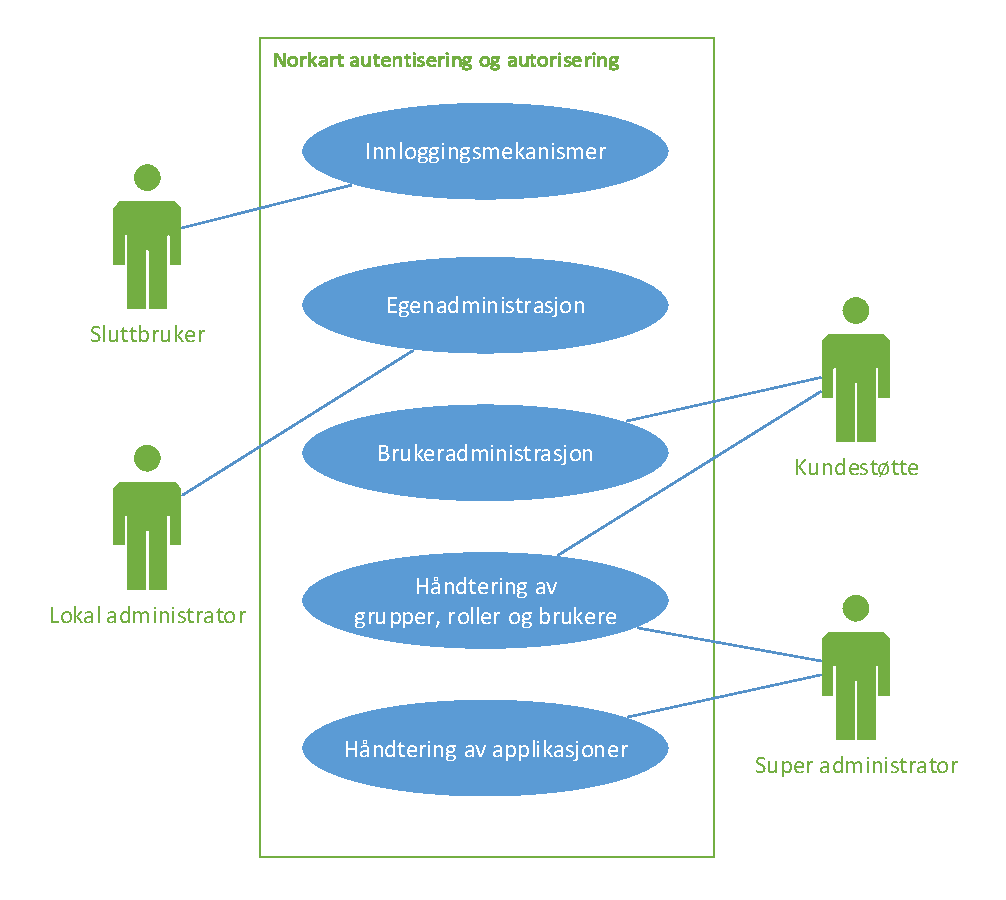
\includegraphics[scale=0.65]{graphics/OverordnetUseCase}
        \caption{overordnet Use Case for autentisering- og autoriseringløsning til Norkart}
        \label{fig:OverordnetUseCase}
        \end{center}
\end{figure}

\subsubsection*{Super administrator}
Super administrator er rollen som administrerer og konfigurerer AAD. Denne rollen er hovedsakelig ment for utviklere og driftere i Norkart. De vil ha mulighet til å håndtere applikasjoner som skal bruke løsningen i tillegg til å håndtere grupper og roller i AAD. 

\subsubsection*{Kundestøtte}
Kundestøtte rollen vil si de som jobber hos kundestøtte i Norkart. De kan hjelpe brukere med funksjonalitet innen brukeradministrasjon. De kan også håndtere grupper og roller i AAD.

\subsubsection*{Lokal administrator}
Denne rollen har til hensikt å administrere brukere innenfor en gitt gruppe. Det kan enten være en person som jobber hos Norkart eller en lokal administrator innenfor en bedrift som benytter seg av NorkartID. Rollen resulterer i redusert press på Norkart kundestøtte.

\subsubsection*{Sluttbruker}
Sluttbruker bruker løsningen som autentisering og autoriseringtjeneste. Dette er brukerne som logger inn via løsningen og får tilgang til tjenestene Norkart tilbyr. I tillegg til dette har de også tilgang på egenadministrasjon slik at belastningen på kundestøtte hos Norkart reduseres ytterligere.

\subsection{Høynivå use case beskrivelser}
\label{subsec:kravspesifikasjon_funksjonelleKrav_hoyNivaa}
For å skape forståelse rundt hovedfunksjonalitet i løsningen er det utviklet 5 høynivå use case beskrivelser.

\begin{framed}
    \begin{tabular}{l p{9cm}}
        \textbf{Use case:} & Innloggingsmekanismer \\
        \textbf{Aktører:} & Sluttbruker
        \bigskip \\
        \textbf{Mål:} & Aktør skal kunne logge seg inn og få sikker tilgang til ønsket applikasjon. Dette skal være SSO slik at aktør i tillegg blir autentisert for andre applikasjoner aktør har tilgang til. Aktør skal i tillegg kunne logge seg ut av en applikasjon. Det skal også være mulig for aktør å gjenopprette sitt eget passord dersom dette er glemt.
        \bigskip \\
        \textbf{Beskrivelse:} & For å skape oversikt deles innloggingsmekanismer her opp i tre underkategorier, logg inn, logg ut og glemt passord. 
        \bigskip \\ 
        \textit{Logg inn} & Når aktør skriver inn brukernavn og passord skal aktøren autentiseres og få tilgang til applikasjonen det ønskes å jobbe på. Da skal aktøren også bli autentisert for andre applikasjoner uten å måtte oppgi brukernavn og passord på nytt. Det vil altså si at det skal være en SSO løsning. 
        \bigskip \\
        \textit{Logg ut} & Når aktør klikker logg ut skal brukeren bli utlogget fra applikasjonen.
        \bigskip \\
        \textit{Glemt passord} & Hvis aktør glemmer sitt passord skal det være mulig å gjenopprette sitt eget passord uten å måtte kontakte Norkart kundestøtte. Aktøren skal kunne gjøre dette ved å trykke på en glemt passord lenke på innloggingsiden. Det skal da sendes en verifiseringkode enten via e-post eller telefon. Ved å oppgi denne koden skal aktøren selv kunne opprette et nytt passord.
    \end{tabular}
\end{framed}

\begin{framed}
    \begin{tabular}{l p{9cm}}
        \textbf{Use case:} & Egenadministrasjon \\
        \textbf{Aktører:} & Sluttbruker 
        \bigskip \\
        \textbf{Mål:} & Aktør skal selv kunne endre {\color{red}og registrere?} på egne registrerte opplysninger på sin brukerprofil. 
        \bigskip \\
        \textbf{Beskrivelse:} &  Aktør skal selv kunne endre sitt registrerte mobilnummer, ekstern e-post adresse og sitt passord. For å endre passord må aktør først oppgi sitt gamle passord, for deretter å skrive inn det nye passordet to ganger. Aktør får kun tilgang til å endre egne data etter å ha blitt autentisert. Egenadministrasjon skal foregå i en ekstern brukerportal, altså ikke i Azure portalen.
    \end{tabular}
\end{framed}

\begin{framed}
    \begin{tabular}{l p{9cm}}
        \textbf{Use case:} & Brukeradministrasjon \\
        \textbf{Aktører:} & Lokal administrator og kundestøtte 
        \bigskip \\
        \textbf{Mål:} & Håndtere brukere innenfor en gitt gruppe.  
        \bigskip \\
        \textbf{Beskrivelse:} & Aktør skal kunne registrere brukere og legge disse til i grupper aktør har tilgang til. Aktør skal i tillegg kunne resette passord for brukerne som er registrert i disse gruppene. Dette skal kunne gjøres fra en egen nettside.
    \end{tabular}
\end{framed}

\begin{framed}
    \begin{tabular}{l p{9cm}}
        \textbf{Use case:} & Håndtering av grupper, roller og brukere \\
        \textbf{Aktører:} & Kundestøtte og super administrator 
        \bigskip \\
        \textbf{Mål:} & Aktør skal kunne registrere og håndtere brukere, grupper og roller.
        \bigskip \\
        \textbf{Beskrivelse:} & For å skape oversikt beskrives brukere, grupper og roller hver for seg.
        \bigskip \\
        \textit{Brukere} & Aktør skal kunne registrere enkeltbrukere i AAD. I tillegg skal det være mulig å masseregistrere brukere fra en ekstern kilde. Aktør skal også kunne legge brukere til i grupper, tildele roller til brukerne og administrere brukernes tilgang til applikasjoner. Dette skal kunne gjøres i Azure portalen.
        \bigskip \\
        \textit{Grupper} & Aktør skal kunne opprette grupper og administrere disse i Azure portalen slik at Norkart kan ha plassere brukere i grupper med forskjellige rettigheter og tilganger. 
        \bigskip \\
        \textit{Roller} & Aktør skal kunne opprette roller med forskjellige rettigheter og tildele disse til brukere som er registrert i AAD. I tillegg skal aktør kunne konfigurere rettigheter og tilganger for eksisterende roller.
    \end{tabular}
\end{framed}

\begin{framed}
    \begin{tabular}{l p{9cm}}
        \textbf{Use case:} & Håndtering av applikasjoner \\
        \textbf{Aktører:} & Super administrator
        \bigskip \\
        \textbf{Mål:} & Aktør skal kunne registrere og administrere applikasjoner i en AAD. I tillegg skal aktør kunne klargjøre applikasjoner for bruk av løsningen.
        \bigskip \\
        \textbf{Beskrivelse:} & I Azure portalen skal aktør kunne registrere web applikasjoner og native applikasjoner for bruk av autentiseringløsningen. Aktør skal også kunne administrere applikasjonenes tilganger og annen informasjon her. I tillegg skal aktør kunne klargjøre og implementere nødvendig logikk i applikasjonene som skal bruke løsningen.
    \end{tabular}
\end{framed}

\section{Operasjonelle krav til løsning}
\label{sec:kravspesifikasjon_operasjonelleKrav}
Operasjonelle krav brukes for å beskrive kvaliteten på systemet og dette kan være i form av standarder som benyttes eller målinger innenfor en gitt grense og kostnader.

\subsection{Ytelse}
\label{subsec:kravspesifikasjon_operasjonelleKrav_ytelse}
\begin{itemize}
\item Løsningen skal som minimum takle 10 000 brukere innlogget samtidig.
\item Løsningen skal håndtere pålogging av 100 brukere i minuttet.
\item Løsningen skal bygges for å være skalerbar.
\item Verifiseringskode for resetting av passord skal mottas innen 20 sekunder for både e-post og telefon.
\end{itemize}

\subsection{Brukervennlighet}
\label{subsec:kravspesifikasjon_operasjonelleKrav_brukervennlighet}
\begin{itemize}
\item Løsningen skal følge regler for universell utforming, se Lover og regler \ref{subsec:kravspesifikasjon_operasjonelleKrav_loverOgRegler}
\item Bruker skal kunne bruke samme pålogginginformasjon mot alle systemene til Norkart.
\item Innloggingsmekanismer som å logge innog egenadministrasjon, se høynivå use case beskrivelse \ref{subsec:kravspesifikasjon_funksjonelleKrav_hoyNivaa}, skal kunne utføres uten opplæring.
\item Brukergrensesnittet, heretter GUI, på innloggingssiden skal være så intuitivt at det tar mindre enn 2 sekunder å skjønne hvor brukerid felt, passord felt og innloggingknappen er.
\item Etter at innloggingsknappen er trykt skal det ta mindre enn 2 sekunder før brukeren ser at noe skjer.
\item Logg ut knappen skal være synlig for bruker i hele applikasjonen
\item Brukeren skal få respons på at utlogging er utført.
\item Når bruker lager passord skal det gis indikasjon på om passordkravene tilfredstilles
\item Brukerprofil for egenadministrasjon skal være oversiktlig og brukeren skal selv skjønne hva som skal gjøres for å endre brukerdata.
\item GUI for all konfigurering av AAD skal være oversiktlig nok til at bruker kan utføre use casene håndtering av brukere, grupper og roller og håndtering av applikasjoner etter å ha fått innføring i Azure eller lest rapporten.
\item GUI design skal skape gjenkjennelighet til Norkart for sluutbrukere. 
\item GUI skal være intuitivt på alle skjermstørrelser..
\end{itemize}

\subsection{Intraoperabilitet}
\label{subsec:kravspesifikasjon_operasjonelleKrav_intraoperabilitet}
\begin{itemize}
\item Brukergrensesnitt på løsningen skal være responsivt.
\end{itemize}

\subsection{Sikkerhet og autentiseringskrav}
\label{subsec:kravspesifikasjon_operasjonelleKrav_sikkerhet}

\begin{itemize}
\item Brukerdata løsningen trenger: Fullt navn, selskap, mail, passord, mobil, sist innlogget og gjeldende autentiserte enheter. 
\item All lagring av brukerdata skal beskyttes i forhold til trusselbilde. 
\item Ingen passord skal sendes eller lagres i klartekst.
\item Systemet skal følge generelle normer innenfor autentisering
\item Minimumskrav for passordlengde er 8 tegn.
\item Minimumskrav for passordkompleksitet er minimum en stor og en liten bokstav, og minimum et tall. 
\item Etter 5 feilede innloggingsforsøk mot en bruker id skal det legges inn ventetid på 1 minutt før det tillattes nytt innloggingsforsøk mot samme bruker id.
\item Ved feil passord eller brukernavn skal det kun stå at innlogging feilet. 
\item Ved glemt passord skal det sendes link til bruker for generering av nytt passord. Denne linken skal kun være gyldig i 20 minutter.
\item En sesjon er kun gyldig 6 timer før den må fornyes.
\item En bruker som logger inn via en nettleser  autentiseres for alle web applikasjoner brukeren har tilgang til i den nettleseren.
\item En bruker som logger inn i en mobil applikasjon autentiserers kun til denne applikasjonen
\item En bruker som logger inn i en desktop applikasjon autentiseres kun til denne applikasjonen.
\end{itemize}

\subsection{Lover og regler}
\label{subsec:kravspesifikasjon_operasjonelleKrav_loverOgRegler}
\begin{itemize}
\item Løsningen skal følge diskriminerings- og tilgjengelighetsloven, kap 3, §13 om Universell utforming.
\item Løsningen utformes i samsvar med standard Web Content Accessibility Guidelines 2.0 (WCAG 2.0) og dermed følge § 4.Krav til utforming av IKT-løsninger i norsk forskrift om universell utforming av informasjons- og kommunikasjonsteknologiske (IKT)-løsninger. 

\end{itemize}

\begin{itemize}
\item Brukerdataløsningen trenger: Fullt navn, selskap, mail, passord, mobil.
\item Ingen passord skal sendes eller lagres i klartekst.
\item Minimumskrav for passordlengde er 8 tegn.
\item Minimumskrav for passordkompleksitet er minimum en stor og en liten bokstav, og minimum et tall. 
\item Ved feil passord eller brukernavn skal det kun stå at innlogging feilet. 
\item En bruker som logger inn via en nettleser autentiseres for alle web applikasjoner brukeren har tilgang til i den nettleseren.
\item En bruker som logger inn i en mobil applikasjon autentiseres kun til denne applikasjonen.
\end{itemize}

\subsection{Klientkrav}
\label{subsec:kravspesifikasjon_operasjonelleKrav_klientkrav}
\begin{itemize}
\item Det kreves at klienten har tilgang på en nettleser som leser HTML5, CSS3 og JavaScript.
\item Klienten må gi tilgang til cookies for å bruke Single Sign On funksjonaliteten i nettleser.
\item Det kreves at klienten er tilkoblet Internett.
\end{itemize}


\section{Krav til resultat av prosjektoppgaven}
\label{sec:kravspesifikasjon_kravTilResultatAvProsjektoppgaven}
{\color{red}TODO}\\
Oppgaven skal skrives etter regningslinjer gitt for bachelor og masteroppgaver ved Høyskolen i Gjøvik.
\\
\\
\href{http://www.hig.no/content/download/30554/364363/file/Retningslinjer%20for%20mastergradsoppgaver%20og%20st%C3%B8rre%20studentoppgaver%20p%C3%A5%20bachelorniv%C3%A5%20ved%20H%C3%B8gskolen%20i%20Gj%C3%B8vik_des2010_v1201.pdf}{Link til retingslinjene}
\chapter{Teoridel}
\label{chap:teoridel}
Dette kapittelet er ment som et oppslagsverk for resten av rapporten, ettersom rapporten er bassert på mye teknologi som var ukjent for prosjektgruppen samt at oppdragsgiver har ytret ønske om en oppsummert innføring om ulike teknologier og begreper som omtales i rapporten. 

\section{Autentisering}
\label{sec:teoridel_autentisering}
Definisjonsjon på autentisering:
\\
\begin{quote}
Å bevise at man er den man utgir seg for å være. Autentisering skal bekrefte en påstått identitet. Dette kan skje gjennom noe du vet (passord), noe du er (fingeravtrykk/ biometri) eller noe du har (nøkkelkort). Kombinasjoner av disse er også mye brukt. Den som autentiseres kan være en person som bruker en datamaskin, kun en datamaskin eller et program.
\end{quote}
\\
Kilde: Norsk senter for informasjons sikring (NorSIS) \cite{NorsisLeksikonAutentisering}.
\\
\\
I denne rapporten er autentisering knyttet til menneske-til-maskin og maskin-til-maskin autentisering. Det er også en form for autentisering som kalles menneske-til-menneske autentisering. Dette kan være bruk av pass og signatur kontroll for at du som menneske, bekrefter ovenfor et annet menneske at du er den du utgir deg for å være. Historisk sett kan vi sammenligne autentiseringsproblematikken med og bekrefte eller avkrefte om en gjenstand er laget av et menneske som påstår at gjenstanden er laget av han. Den samme utfordringen må løses i maskinverden for og autentisere på en sikker måte.

\subsection*{Prinsipp}
Menneske-til-maskin autentisering er noe som foregår mellom et menneske, typisk en bruker av maskinressurs og en maskin, som inneholder eller gir tilgang til maskinressursen. Som bruker av en maskinressurs skal man bekrefte for maskinen at du er den du utgir deg for å være, man lager da egne brukere for hver enkelt bruker av maskinressursen. En bruker kan gi seg til kjenne ved å oppgi et brukernavn og et passord. Om maskinen gjenkjenner brukernavn og passord fra tidligere oppgitte brukerprofiler vil maskinen tillatte tilgang til maskinressursen. Om man bruker passord for og bekrefte at du er eieren av brukernavnet så kaller vi ofte passordet for nøkkelen, om man bruker fingeravtrykk eller ansiktsgjekjenning regnes dette som nøkklene. En maskinressurs kan eksempelvis være en smarttelefon, en webapplikasjon eller et operativsystem, man kan i prinsippet autentiseres for å få tilgang til hva som helst av beskyttet innhold.
\\
\\
Maskin-til-maskin autentisering gjøres på nesten samme måte som menneske-til-maskin, forskjellen er bare at maskinene har lagret nøkkelen på forhånd. Det er ulike former for metoder og teknologier som kan brukes for og beskytte mot misbruk av nøklene som er lagret. Dette skal vi ikke gå inn på i denne rapporten, da dette er noe som blir løst av rammeverkene og protokollene som eventuelt vil bli brukt.  

\subsection*{Utfordringer}
Gitt at brukernavnet skal være enkelt for en bruker å huske, velger bruker ofte et brukernavn som er relativt logsik bygd opp, i forhold til eget navn, stilling eller rolle i systemet brukeren skal ha tilgang til. Dette gjør det enkelt for andre å gjette brukernavnet. Om brukernavnet også er mailaddressen til brukeren, ønsker man kanskje at andre skal vite om brukernavnet ditt også, så man sprer brukernavnet til så mange som mulig. 
\\
\\
Passordet, eller nøkkelen som brukes for og bekrefte at brukeren er den brukeren utgir seg for å være bør også være noe som brukeren enkelt kan huske. Ideelt sett så skal denne nøkkelen være noe som er enkelt for brukeren og huske eller bevise, men vanskelig for andre og gjette eller simulere. Sikkerhetsrapporter og undersøkelser viser at mennesker ser ut til å være så redd for å glemme passordet sitt at de velger heller et enkelt passord, framfor et vanskelig som vil beskytte brukerkontoen mye bedre mot uautorisert bruk. Et eksempel på en rapport som viser dette er Trustware sin Global Security Report fra 2014 \cite{TruswareGlobalSecurityReport2014}. Denne rapporten påstår at en tredjedel av alle saker knyttet til uautorisert tilgang de etterforsket i 2014, var som følge av et svakt passord. En god autentiseringsmekanisme bør derfor kreve at brukeren må lage et sterkt passord og eventult at brukeren autentiserer seg med andre metoder enn bare passord. Eksempelvis engangskoder man får på SMS, fingeravtrykk eller ansikstgjenkjenning. 
\\
\\
Det er mulig å designe et system som hjelper brukere og være flinke til å velge sterkere nøkkel. I tillegg kan vi designe autentiseringssystemet slik at det kreves to-faktor autentisering for og autentiseres. To-faktor kan brukes hver gang man forsøker å autentisere seg, eller bare ved tilfeldig utvalgte autentiseringsforsøk.

\section{Autorisasjon}
\label{sec:teoridel_autorisasjon}
Definisjonsjon på autorisering: \\
\begin{quote}
Autorisering er prosessen med å beslutte å gi en person, en datamaskin eller et program tillatelse til å bruke bestemte IT-ressurser. Eksempler på en IT-ressurs kan være filer, nettverksstasjoner og prosesser.
\end{quote} \\
Kilde: Norsk senter for informasjons sikring (NorSIS) \cite{NorsisLeksikonAutorisering}. \\
\subsection*{Prinsipper}
Autorisasjon i forhold til datasystemer dreier seg om å avgjøre hva en bruker skal få tilgang til og ikke. En autorisasjon skjer etter at en bruker er vellykket autentisert (se seksjon \ref{sec:teoridel_autentisering}). Vi kan dele autorisasjonsprosessen inn i to faser. Første fase er og avgjøre hva en bruker skal ha tilgang til og ikke, altså å definere tilganger, vi kaller dette definisjonsfasen. Andre fase er og godkjenne eller ikke godkjenne forespørsler om tilgang til ressurser bassert på hva som er definert i fase 1, vi kaller dette godkjenningsfasen. Alle tilganger ligger i en form for brukerdatabase, denne kan være implementert på svært ulike måter avhengig av system og bruk. \\
\\
Datasystemer bruker autorisasjon for og skille brukere fra hverandre, slik at brukere og brukergrupper kun har tilgang til ressurser de er godkjent for å ha tilgang til.

\subsection*{Utfordringer}
Definisjonsfasen av et system kan være utfordrende når det er mange grupper og medlemmer i brukerdatabasen.  Det å ha kontroll på hva ulike grupper og medlemmer skal ha tilgang til, å kanskje spesielt hva de ikke skal ha tilgang til kan fort bli en krevende jobb. Det er derfor vanlig og definere reglene i en form for policy. De som tradisjonelt har utført tilgangstildelinger i definisjonsfasen er administratorer og brukerdatabase eksperter.  \\
\\
Det kan tenkes at det ikke nødvendigvis er administratoren for brukerdatabasen som vet om brukeren faktisk skal få tilgang eller ikke. Dersom administratoren må dobbeltsjekke at brukeren kan få tilgang til en gruppe fra gruppeeier, før brukeren får tilgangen innvilget, vil dette kunne ta tid. Et godt autoriseringssystem gir spesielt utvalgte brukere i ulike grupper, ofte kalt gruppeeiere, tilgang til og fjerne eller legge til rettigheter på andre brukere for bestemte grupper. Om brukeradministrasjonssystemet gir mulighet for slike gruppeeiere, bør systemet designes for å være så enkelt som mulig for å hindre uønskede brukerfeil av gruppeiere.

\section{Single Sign On}
\label{sec:teoridel_singleSignOn}
SingleSignOn (SSO) er et begrep for å beskrive at man kan bruke en brukerautentisering som allerede er vellykket for å automatisk logge deg inn på andre tilknyttede systemer. Når et system har denne egenskapen kan en bruker logge inn en gang og få tilgang til andre systemer uten å bli spurt igjen om å logge inn på hver av dem\cite{SSOLogg}. Typisk blir dette håndtert ved bruk av en Lightweight Directory Access Protocol\cite{SSOLDAP}(LDAP\footnote{Lightweight Directory Access Protocol (LDAP) er en protokoll som brukes til oppslag i en katalogtjeneste på en server.}) og en database med brukere. \\
\\
SingleSignOn er vanlig på intranett nivå eksempelvis internt i en bedrift, de siste årene har det blitt mer vanlig med implementasjon av "identity providere" som gjør det mulig å bruke en brukers identitet i en annen applikasjon for å logge inn på tilknyttede applikasjoner. To eksempler på selskaper som tilbyr dette er facebook og google, begge selskapene gir muligheter for andre applikasjoner å bruke dem som identity providere, slik at brukerene får en følelse av SingleSignOn. Ofte må brukerne her fortelle applikasjonen at brukeren ønsker å logge inn ved bruk av eksisterende autentisering igjennom facebook eller google. Denne type innlogging gir heller ikke alltid samme sikkerhet for SingleSignOut, det er ikke gitt at om du logger ut fra facebook eller gooogle kontoen din at du logger ut fra applikasjonene som har brukt dem som "identity providere". \\
\\
Siden ulike autentiseringsmekasnismer fungerer på ulike måter må en SSO tjeneste lagre og oversette legitimasjon den mottar fra sin første autentisering og sende den til alle tjenestene det måtte gjelde. Det er viktig at identitetshåndteringen relatert med SSO løsningen holdes oppdatert i alle ledd angående autentisering da det er viktig å få spredd endringer og nye opprettelser av identiter. \cite{SSOProblemer}

\section{Microsoft Active Directory}
\label{sec:teoridel_microsoftActiveDirectory}
Microsoft Active Directory (AD) er en LDAP server, altså en katalogtjeneste fra Microsoft. Den brukes for å tildele ressurser til brukere og brukergrupper, både eksternt og internt, i en bedrift. AD kan sees på som en spesialdesignet database som er designet for å fungere veldig godt på små lese og søke operasjoner men ikke så godt på endringer og oppdateringer av. AD er bygd opp av objekter. Et objekt kan være et system, en ressurs eller en tjeneste.\cite{AD}\\
\\
AD ble lansert i 1999, i Windows Server 2000 og har siden det gradvis blitt forbedret og videreutviklet i takt med nyere versjoner av operativsystemer fra Microsoft. Azure Active Directory kan sees på som siste versjon av AD, denne er kun tilgjengelig i Azureskyen til Microsoft, altså kun over internett. Les mer om Azure Active Directory i delkapittel \ref{sec:teoridel_azureAd}.

\section{SAML}
\label{sec:teoridel_SAML}
SAML står for Security Assertion Markup Language og er et XML-basert\footnote{Exstensible Markup Language, et universelt og utvidbart markeringsspråk. Brukes for deling av data mellom systemer, spesielt over internett og for koding av dokumenter.}  åpen autentiserings protokoll. Det viktigste SAML adresserer er nettleser single sign-on (SSO). SAML fungerer ved at den definerer tre roller: 
\begin{itemize}
\item Bruker
\item Identitetstilbyder 
\item Tjenestetilbyder (applikasjon)
\end{itemize}
Se kapittel \ref{subsec:konfigurasjon_innloggingsmekanismer_hvaSkerVedInnlogging} for en beskrivelse av autentiseringsflyten i for SAML protokollen. Kommunikasjonmetoden som SAML bruker er XML kombinert med ulike kommunikasjons protokoller\cite{SAMLProtokoller} som HTTP og SOAP\footnote{Er en protokoll for utveksling av XML-baserte meldinger}. SAML ble definert av OASIS SSTC (Security Services Technical Committee) i Januar 2001\cite{SAMLHist}. Protokollen er revidert flere ganger og har endt opp i versjonen, SAML 2.0, som ble en standard i 2005. \\
\\
SAML er enda aktuell autentiseringprotokoll for en rekke tjenester. Det er identitetstilbydere som kun tilbyr SAML som ønsker å knyttes til nye applikasjoner, og nye applikasjoner som ønsker å gi mulighet for å knyttes til vi SAML. Våren 2015 ble det lagt inn støtte for SAML i nye Office 365 fra Microsoft\cite{SAMLOffice}. 
\section{WS-Federation}
\label{sec:teoridel_WSFederation}
Dette er en protokoll for kommunikasjon mellom Identity Providers\footnote{Tilbyder av identitet for brukere som ønsker å interaktere med et system.} og Relying Parties\footnote{Databegrep for å snakke om en server som gir tilgang til en sikret software applikasjon.}. Den definerer et rammeverk for spørringer relatert med forespørseler om tilgang til en beskyttet ressurs. Målet med WS-Federation er å forenkle utviklingen av fødererte tjenester igjennom intern og fjern kommunikasjon og håndtering av disse tjenester ved å bruke WS-Trust Security Token. WS-Trust er en spesifikasjon og en OASIS-standard som håndterer utlevering, fornying og validering av sikkerhets tokens. Den bruker samme innkapslingsmetode som WS-Trust nemlig RST/RSTR\footnote{RST står for Request Security Token og RSTR står for Request Security Token Response og er standard kommunikasjons meldinger som brukes av WS-Federation.}. \\
\\
Lansert i 2003 og revidert til versjon 1.2 i 2009. WS-federation brukes i dag i relasjon med Single Sign-On og autentiseringsløsninger.

\section{OAuth 2.0 \& OAuth 1.0}
\label{sec:teoridel_oauth}
OAuth 2.0 er en åpen protokoll for autentisering og autorisering av beskyttet innhold. Protokollen er basert på bruk av tokens som har ulik funksjonalitet. Protokollen er bygget for å ha lav overhead i forhold til for eksempel SAML. Den er designet spesifikt til å fungere over Hypertext Transfer Protocol (HTTP). OAuth bruker "Refresh tokens", "Access tokens" og "Access code" for å oppnå at applikasjoner kan bruke identitetstilbydere for autentisering av brukere. I kapittel \ref{subsec:konfigurasjon_innloggingsmekanismer_hvaSkerVedInnlogging} beskrives autentiseringsflyten og tokenene nærmere. \\
\\
OAuth ble utviklet i 2006 da en utvikler jobbet med OpenID implementering mot Twitter. Dette senere resulterte i 2007 i OAuth 1.0.\cite{OAuth10Hist} Sammenlignet med OAuth 2.0 så er protokollen lettere å implementere på sin applikasjon og førte inn SSL i alle ledd av komminkasjon. I OAuth 1.0 ble alt kodet og dekodet som en rekke signaturer som førte til mye behandlingstid for alle forespørsler. Siden SSL sikrer dette uten å måtte gjøre denne jobben så er det høyere ytelse i 2.0.\cite{OAuthDifferences} OAuth 2.0 ble lansert i 2012.  \\
\\
Protokollen er bassert på REST\footnote{REST står for Representational State Transfer og er en software arkitekts stil som følger retningslinjer og best practice for å lage skalerbare web tjenester.} og JSON\footnote{JSON står for JavaScript Object Notation og er en enkel tekstbasert standard for datautveksling.} noe som åpner for enkel bruk av protokollen fra både datamaskiner, mobile enheter, smartklokker og annet utstyr med støtte for disse protokollene.

\section{Azure AD Graph}
\label{sec:teoridel_azureAd_graph}
Azure AD Graph er en API protokoll som lar autoriserte brukere gjøre operasjoner på objekter i Azure AD. Datastrukturen i Azure AD er bygd opp som en graf. AAD Graph tillater autoriserte brukere å gjøre spørringer mot AAD for å oppdatere eller navigere igjennom objektene i AAD. Objektene i ADD, altså brukere, grupper og applikasjoner kan sees på som objekter som er knyttet til hverandre med koblinger. Objektene kan også kalles noder.  Protokollen er kommuniserer ved bruk av REST og JSON meldinger. \\
\\
Protokollen sammenlignes med Facebook Graph API. Facebook har mer funksjonalitet og muligheter bygget inn i sin Graph, men prinsippene er det samme. Man kan hente ut, legge til, oppdatere eller slette informasjon som ligger i noder i datastrukturen i brukerdatabasen. Denne funksjonaliteten bidrar til å skape et stort skille mellom hva en tradisjonell AD kan gjøre og hva AAD kan gjøre for både administratorer, sluttbrukere og utviklere. Graph API gjør det mulig å lage webapplikasjoner som kan jobbe rett på objektene i AAD uten å trenge noen form for ekstra mellomvare annet enn det som allerede er bygget inn i Azure AD.

\subsection*{Tilganger}
For og hindre at alle brukere kan gjøre alle operasjoner er det tilgangsstyring på hva brukere kan gjøre med AAD igjennom graph. Dette gir i prinsippet mulighet til å delegere tilganger og lage tilgangsgrupper som har lov til å endre og gjøre ulike ting igjennom graph API. Dette er funksjonalitet som man ikke enda kan gjøre igjennom eksisterende portaler tilknyttet AAD. Microsoft har varslet at slik funksjonalitet vil komme \cite{NasosAzureADExplained}, men sier ingenting om når og hvordan. 


\section{OpenID Connect}
\label{sec:teoridel_openIdConnect}
OpenID Connect (OIDC) er en åpen identitets protokoll som ligger på toppen av OAuth 2.0. Den muliggjør for klienter å kunne verifisere identiteten til en sluttbruker ved hjelp av en id token. OpenID Connect bekrefter identitenen på brukeren som er autentisert med svært lav overhead i forhold til andre autentiseringssystemer\cite{OIDCFunksjonalitet}. OIDC er utviklet med mål om å “making simple things simple and complicated things possible”\cite{OIDCHjemmeside}. Det muliggjør for utviklere å autentisere sine brukere på tvers av nettsider og applikasjoner uten å måtte eie og håndtere passord eller autentiseringsmekanismer selv på en enda enklere måte enn bare ved bruk av OAuth. Ettersom protokollen er satt sammen av blant annet flere elementer har man også fordelene og egenskapene ved bruk av OAuth også, dette betyr blant annet kommunikasjon ved bruk av REST og JSON meldinger. 

\section{Azure}
\label{sec:teoridel_azure}
Microsoft Azure er sky plattformen til Microsoft. Azure er hovedsakelig en skytjeneste men deler av funksjonaliteten kan også bygges på private servere. Plattformen er bygd for å levere Infrastructure-as-a-Service (IaaS) og platform-as-a-service(PaaS). Dette muliggjør at du kan ha både managed og unmanaged tjenester. Managed menes at du kan ta å sette opp en tjeneste fra bunnen av og du har kontroll og oversikt i alle ledd av en tjeneste, dette betyr konfigurasjon av operativsystem, programvare og annet. Unmanaged betyr at du henter ut en service direkte i Azure og bruker tjenesten direkte som en abstrakt entitet, du oppretter tjenesten ved noen få tastetrykk og kan ta ibruk tjenesten med en gang. Azure kan sees på et samlepunkt for alle server-tjenester Microsoft har tilgjengelig med en oversiktlig “webdrakt” utenpå. Ved å bruk en slik løsning har du tilgang til alle aspekter man har ved viritualisering men man kan også ta i bruke tjenester direkte uten å måtte sette dem opp selv på en virtuell maskin. Med Azure kan du bygge infrastruktur, utvikle moderne applikasjoner, få innsikt i samt behandle data og håndtere identitet og tilganger. 
\\
\\
Tjenesten ble lansert i 2010 og hatt stødig vekst siden\cite{AzureLansert}. Azure blir idag brukt til å løse infrastruktur utfordringer og muliggjør for mindre bedrifter å kunne tilby tjenester på en dynamisk skalerbar måte, uten å trenge å drifte, oppdatere eller vedlikeholde operativsystemene og programvaren selv. 
\\
\\
Utfordringer rundt Azure er det lovmessige aspektet som bedrifter generelt står ovenfor når de skal ta i bruk skyløsning. Når data er lagret i skyen vil det tidvis være uklart hvilke regler som gjelder for ulike typer håndtering av data. Om selskapet er registrert i Norge, Azure serverene som brukes står i Irland men Microsoft er registert som et Amerikansk selskap så må man forholde seg til lovverk fra alle tre landene. Microsoft etterstreber å møte nasjonale og internasjonal standarder slik at sikkerhetsnivået, regler og rutiner overholdes på en god måte\cite{AzurePrivacy}. På tross av dette er lovverk rundt personopplysninger i Norge fortsatt så streng at det er en utfordring og benytte seg av utenlandske selskaper for lagring av den sensitive informasjonen. Det er ulike måter å løse denne problemstillingen på, men prosjektgruppen har valgt å ikke gå dypere inn i dette i enne oppgaven.

\section{Azure AD}
\label{sec:teoridel_azureAd}
Azure Active Directory (Azure AD eller AAD) den nye skyversjonen av Microsoft Active Directory. Azure AD er designet for å dekke identitet- og tilganghåndtering for en bedrift både for intranett og i skyen. Den lar deg lage en egen privat katalogtjeneste for håndtering av eksterne og lokale ressurser og tilganger. ADD er kun tilgjengelig i skyen, og er ikke bare en katalogtjeneste slik som Active Directory. Av ny funksjonalitet er integrerte påloggingsprotokoller for SSO av applikasjoner knyttet til Azure. Disse applikasjonene kan være utviklet selv, eller tilknyttet AAD fra før. Microsoft jobber hele tiden med å legge til nye applikasjoner for SSO i sin tjeneste, og har som mål at alle store nettapplikasjoner skal være tilgjengelige for deres brukere igjennom AAD. For bedrifter som allerede benytter Microsfot Office 365 er tjenesten inkludert i lisensen. Azure AD lisensieres på ulike måter, les mer om dette i kapittel \ref{subsec:konfigurasjon_genrellHaandteringAvAad_lisensmodell}.
\\
\\
Azure AD kobles opp mot et sett av ulike tjenester med ferdig konfigurert “endpoints” eller api’er for tilkobling av ulike tjenester. Dette gjelder blant annet OAuth 2.0, OpenID Connect, SAML, AD Sync med flere. Azure AD kan fungere som en mer tradisjonell Active Directory eller den kan brukes mer rettet mot web applikasjoner eller native applikasjoner. 
\\
\\
AAD har vært tilgjengelig like lenge som Azure. Microsoft mener framtiden er i skyen og Azure AD er deres svar på identitetshåndtering. Ved å bruke Azure AD har man tilgang til sikkerhet og beskyttelsesmekanismer Microsoft har jobbet lenge med å implementere og bygge opp på en god måte, dette er ingen hvilepute, men hjelper når bedrifter skal tenke sikkerhet for datasystemene sine.

\section{IdentityServer3}
\label{sec:teoridel_identityServer3}
Identityserver3 er et OpenSource .NET/Katana basert rammeverk for implementering av OpenID Connect. Rammeverket er bygget så man må bygge knytningen til brukerdatabasen og deler av gui'en selv. Men rammeverket muliggjør implementering av Single Sign-On og tilgangkontroll for moderne web applikasjoner og API's ved bruk av protokollene OpenID Connect og OAuth2. Ved bruk av OpenID Connect gir dette mulighet for at rammeverket kan brukes på ulike klienter deriblant mobil, web, SPA\footnote{Single-Page Application (SPA), er en web applikasjon eller web side som passer på en enkel web page med mål om å gi bruker en flytenede bruker opplevelse på lik linje som en skrivebordsapplikasjon. I en SPA blir all kode, HTML, Javascript og CSS hentet ned i nedlastningsøyeblikket eller blir hentet dynamisk og lagt til i siden ved behov.} og skrivebordsapplikasjoner. 
\\
\\
IdentityServer3 er det tredje OpenSource prosjektet bygget av flere av de samme menneskene. Tidligere versjoner av IdentityServer har implementert eldre protokoller. Navnet IdentityServer3 kommer av at det er det tredje prosjektet og ikke 3. versjon av programvaren, IdentityServer3 1.0 har vært tilgjengelig siden Februar 2015, mens IdentityServer 2.0 Beta har vært i betatest siden April 2015. Det er nå det tyske selskapet tyske selskapet Thinktecture med Dominick Baier i spissen som driver prosjektet og jobber med å forbedre og videreutvikle fortløpende\cite{IDServV3Hist}. Rammeverket er gjennomtestet og utviklerne av rammeverket ser ut til å være faglig svært sterke. I motsetning til Azure AD kreves det mer kompetanse i form av kodeferdigheter og forståelse for autentiseringsmekansimer å sette opp en løsning bassert på IdentityServer3. Løsningen koster ikke noe annet en utviklingstid å ta i bruk, men ettersom dette er et OpenSource prosjekt er framtiden for prosjektet noe usikker. Man kan aldri helt være sikker på om det vil fortsette å bli vedlikeholt, selv om det er en trygghet i at det er et selskap med tung it kompetanse som er tett knyttet til prosjektet.   

\section{OWIN og Katana}
\label{sec:teoridel_owinOgKatana}
{\color{blue}Er dette skrevet av fra et sted?}\\
{\color{red}Så OWIN er en opensource comunity drevet standard som gjør det mulig å implementere .NET applikasjoner på hvilken som helst webserver? Katana er en openspource implementasjon av standarden hvor utviklingene er dervet av Microsoft?}
\\
\\
OWIN er spesifikasjoner for å separere kommunikasjonen mellom .NET web applikasjoner og servere opp i moduler. OWIN regnes som en standard og er opensource og "comunity drevet". Hensikten med OWIN prosjektet var å skille ut komponenter Microsoft tidligere hadde bygget inn i .NET kjernen, så de ble tilgjengelige for alle webservere å håndtere. 

kun er spesifikasjoner brukes Katana for å implementere disse spesifikasjonene. Katana er et fleksibelt sett av komponenter for bygging og drifting av OWIN-baserte web applikasjoner. Komponentene er opensource OWIN komponenter som er bygget og sluppet av Microsoft. Disse komponentene inkluderer både infrastruktur biter som hosts og serveres, og i tillegg funksjonskomponenter, som autentiserings og tilknytningsmuligheter til andre rammeverk som er i ASP.NET Web. Poenget med Katana er at det skal være portabelt, modulært og skalerbart samt lettkjørt. Målet med dette prosjektet er at det skal være et abstraksjonlag mellom .NET web servere og web applikasjoner for å gi utvilkere flere valgmuligheter enn det som har vært tidligere. Prosjektet muliggjør utviklere om å bestemme hvor lettkjørt eller hvor funksjonsrikt Web løsningen skal være. Katana er en implementering av OWIN spesifikasjonene, gjennomført av Microsoft. \\

Katana 

\section{Azure AD Application Proxy}
\label{sec:teoridel_azure_ad_application_proxy}
Azure AD Application Proxy er en tjeneste i Azure AD som eksponere web applikasjoner, eksempelvis Outlook Web Access og IIS-baserte applikasjoner, i et privat nettverk til eksterne brukere. Dette fører til at brukere kan sikkert aksessere applikasjoner autentisert fra hjemmet og på sine egne enheter. Dette fører til at brukerne kan autentisere igjennom en skybasert proxy som blir driftet i Azure og få tilgang. Eksterne maskiner kan utføre sikker tilkobling til organisasjonen sine nett-tjenester uten bruk av VPN og uten åpne for sikkerhetsproblematikk. \\
\\
Denne tjenesten ble sluppet tidlig desember 2014 og har vært tilgjengelig siden. For å kunne bruke Application Proxy må man ha Azure AD Premium.\\
\\
Oppsette på dette vil være at man har en server med en singel applikasjon kjørende. Denne blir sett på som en connector og den lager en outbound tilkobling til Azure løsningen man har og avventer videre instrukser. I Azure wil dette dukke opp som en Proxy Applicatoin med både ekstern og intern URL konfigurert og med autentiseringsalternativer. Når en bruker åpner den eksterne URL'en vil denne spørringe blir videresendt til connector serveren som håndterer endelig trafikk mot web serveren. Proxy connectoren lager kun en outbound tilkobling og det er derfor ikke behov for å vise webserveren direkte ved brannmuren.

\section*{Single tenant applikasjon}
\label{sec:singleTenantApplikasjon}
Single tenant betyr at en applikasjon kun kan brukes av en bedrift. For å tilby applikasjonen til flere bedrifter må det lages en ny versjon av applikasjon, database og eventuell lagring for hver enkelte bedrift man selger applikasjonen til. Fordeler gir tilbyder av programvaren enklere mulighet til å tilpasses hver enkelt leveranse av applikasjonen. Man sikrer ytterligere selve adskillelse av data i database og lagring. Dersom en applikasjon skulle feile under en oppdatering eller ved vedlikehold, påvirker ikke dette noen andre bedrifter enn kun de som er knyttet til denne. Ulike ulemper vil være at det vil ta tid å holde koden for mange like applikasjoner vedlike dersom det er gjort store tilpasninger på hver og en. I tillegg til dette gir det deg flere databaser, flere applikasjoner og potensielt flere servere å vedlikeholde.

\section*{Multi tenant applikasjon}
\label{sec:multiTenantApplikajson}
Multi tenant betyr at applikasjonen kun ligger et sted, men er satt opp for å fungere mot ulike bedrifter. Alle bedriftene og brukerne deler applikasjon, lagring og database. Applikasjonen oppleves som adskilt fra hverandre ved at data blir merket tilhørende ulike brukere eller bedrifter. Applikasjonen skiller mellom hvilken data som tilhører hvilken bedrift. Fordelen ettersom det kun er en instans av applikasjon og applikasjondatabasen vil være at du kun trenger å gjøre en oppdatering på en tjeneste. Dette vil deretter slå ut på samtlige brukere umiddelbart. Vedlikehold vil også bli enklere da du må forholde deg til færre servere og tjenester. Ulemper tidligere så man på multi-tenant løsninger som kompliserte å ta backup av. Dette vil ikke påvirke oppdragsgiver ettersom de betaler Microsoft for hosting og drift og backup, ytterligere backup de gjør selv vil kun være en ekstra sikkerhet. Single point of failure om det skulle være noe som feiler på applikasjonen så har det utslag på alle brukere av gitt applikasjon.

\section{Windows PowerShell}
\label{sec:teoridel_windows_powershell}
Skal vi ha med om dette? Powershell er praktisk i mange sammenhenger for Norkart og ser ut til å være mye brukt i Azure og Windows sammenheng.
\chapter{Valg av løsning}
\label{chap:valgAvLosning}
Dette kapittelet beskriver de to systemene vi så som aktuelle for å løse problemstillingen oppdragsgiver ga oss. Hensikten med kapittelet er å argumentere for valgt løsning, mens utfordringer rundt implementasjonen av valgt løsning drøftes i kapittel \ref{chap:konfigurasjon}.

\section{Mulig løsninger}
\label{sec:valgAvLosning_muligeLosninger}
Prosjektgruppen har i samråd med Product Owner plukket ut to produkter prosjektgruppen har valgt å se nærmere på. Hensikten med dette er å kunne sette dem opp mot hverandre og ta en kunnskapsbasert beslutning om hvilken løsning prosjektgruppen skal fordype seg ytterligere i for å gi oppdragsgiver mest mulig relevant informasjon. De to løsningene som er valgt ut er Azure Active Directory (se kapittel \ref{sec:teoridel_azureAd}) og IdentityServer3 (se kapittel \ref{sec:teoridel_identityServer3}). For enkelhets skyld omtales IndentityServer3 som en ferdig løsning, selv om IndentityServer3 er et rammeverk hvor serveren må bygges og utvikles rundt.
\\
\\
De neste delkapitlene skal forsøke å sette de to valgte løsningene opp mot hverandre for å finne forskjeller og likheter.

\subsection{Implementasjon}
\label{sec:valgAvLosning_muligeLosninger_implementasjon}
I denne seksjonen vil det først drøftes litt rundt de to løsningene hver for seg, for så å trekke noe slutninger i forhold til implementasjon til slutt.

\subsection*{Azure AD}
AAD er ifølge Microsoft en ferdig løsning der brukerne skal ikke trenge å gjøre noe annet enn å legge til brukere, applikasjoner og grupper før løsningen kan tas i bruk. Prosjektgruppen har etter testing av ulike deler av løsningen konkludert med at dette er en sannhet med modifikasjoner. AAD er ganske ferdig, men komplisert å bruke riktig da det krevers kunskap om AD og AAD for å kunne sette opp dette raskt og hensiktsmessig. Det er små valg i konfigurasjonen av løsningen som får svært store konsekvenser om man ikke vet hva man driver med. 
\\
\\
AAD er en unmamaged løsning som vil si at Microsoft drifter løsningen og sørger for at systemet bak løsningen fungerer som det skal. Som eier av en AAD så skal du kun konfigurere og bruke din AAD. 
\\
\\
Microsoft som leverer AAD ønsker å tjene penger. Det er lagt begrensninger i AAD ved at man ikke kan legge til applikasjoner uten at de allerede er tilknyttet Azure på en eller annen måte. Selv om det kan diskuteres hvorvidt løsningen er dyr eller ikke så tar Microsoft seg litt betalt for alt. Betalingsplanene har muligheten til å skalere etter bruk, slik at man kun betaler for det man bruker. Kostnadene skalerer etter hvor mye brukerene bruker systemet, ikke etter hvor mye det koster å implementere eller kjøpe inn systemet.

\subsection*{IdentityServer3}
IdentityServer3 er et open source prosjekt som har som mål å lage et rammeverk for håndtering av OpenID Connect protokollen for ASP.NET prosjekter. Det er en liten gruppe utviklere som står bak prosjektet, og prosjektet har fått mye skryt i ulike blogger og fagmiljøer på nettet. Ettersom IdentityServer3 kun er et rammeverk vil det si at du må bygge mer rundt løsningen for å kunne bruke den med en tjeneste. Prosjektgruppen har testet enkle oppsett med denne løsningen uten å knytte den til noen database. Løsningen virker gjennomarbeidet og god. 
\\
\\
Ettersom identityServer3 ikke er en ferdig løsning som kan tas ibruk med en gang, må det bygges et system rundt rammeverket. Dette må utvikles og implementeres av Norkart selv. Tilknytning, oppsett og konfigurasjon av en brukerdatabase må også gjøres under utviklingen. Utviklerne av implementasjonsløsningen står fritt til å bruke dyre kommersielle databaser og utviklingsverktøy, eller å bruke "free to use" open source løsningner. I teorien skal man kunne bygge en løsning basert på IdentityServer3 helt uten lisenser som koster oppdragsgiver annet enn utvikling og driftskostnader. IdentityServer3 er bygget etter OpenID Connect standarden og gir eier av systemet muligheter til å koble til alle typer applikasjoner så lenge applikasjonen følger OpenID Connect standarden.
\\
\\
Framtiden til open source prosjekter kan være usikker da den er avhengig av at utviklere bruker fritiden sin på å feilrette, utbedre og videreutvikle prosjektene. Dette gjelder også for IdentityServer3 prosjektet. Selv om prosjektet får mye skryt på Internett betyr ikke dette at det er feilfritt, eller at det ikke trengs support på løsningen. 

\subsection*{Slutninger}
Oppdragsgiver er allerede svært tett knyttet til Microsoft. De aller fleste applikasjonene som leveres Norkart idag har tilknytning til Microsoft systemer allerede og dette vil gjelde også for framtidige løsninger. Dette gjør det rimelig å anta at en ytterligere knytning til Microsoft for å få applikasjonene til å fungere over Azure AD er realistisk å få til uten altfor kostbare grep.
\\
\\
Oppdragsgiver er forberedt på å betale for en autentiseringsløsning slik de har etterspurt av prosjektgruppen. Det er en vurderingssak om man skal sette bort hele løsningen til Microsoft for å redusere implementasjonskostnader eller om man skal bruke tid og penger på å utvikle store deler av løsningen selv. 
\\
\\
Support og støtte i forhold til oppsett og konfigurasjon av løsningenene er i skrivende stund varierende. Både IdentityServer3 og AAD er svært nytt da begge har begrenset oppdatert støttedokumentasjon på nett. Det er rimelig å anta at tilgangen på støttedokumentasjon vil bedre seg raskt når det blir enda flere som bruker løsningene. Ettersom Microsoft har god erfaring med å selge ut komplekse løsninger til bedrifter i stor skala er det rimelig å anta at de også vil tilby veiledning, kurs og relevant støttedokumentasjon også til AAD. Norkart er Gold Partner med Microsoft og det resulterer i et allerede tett samarbeid hvor det da vil være enkelt å få tilgang til support for AAD.

\subsection{Driftsaspekter}
\label{sec:valgAvLosning_muligeLosninger_driftsaspekter}
I forhold til drift så skiller de to løsningene seg veldig fra hverandre. AAD driftes nesten utelukkende av Microsoft, mens IndentityServer3 er en løsning Norkart selv står ansvarlig for å bygge, vedlikeholde og drifte. Med AAD trenger man kun vedlikeholde koblingen til applikasjoner og brukeradministrasjon da dette må gjøres uansett. IdentityServer3 vil legge alt driftsansvar på Norkart.
\\
\\
Ved bruk av IdentityServer3 må Norkart selv drifte både autentiseringsserveren og databasen hvor applikasjon- og brukerinformasjon lagres. Fordelen med å drifte alt selv er
\begin{itemize}
\item man vet hvor ting lagres til enhver tid
\item man har mulighet til og kontrollere
\item sikre og tilpasse løsningen slik det passer
\end{itemize}
Ulempen er at implementasjon av slike hjelpemidler og sikringstilltak kan ta tid. Norkart har allerede flere applikasjoner de drifter idag. Drift av IndentityServer3 vil trolig inngå som en del av de etablerte driftsrutinene Norkart allerede har etablert. 
\\
\\
Det er også en tredje mulighet, bygge løsningen selv ved å bruke IndentityServer3 og å hoste løsningen i Microsoft Azure. Det blir da en managed tjeneste da Norkart må fortsatt konfigurere og drifte systemet og løsningen, men Microsoft garanterer oppetid i form av nettlinje og virtuelle maskiner i forhold til sin SLA \footnote{Service Level Agreement(SLA) er en prosess som skal sikre at kunde og leverandør har en felles forståelse for hva som skal leveres, og til hvilken kvalitet.\cite{SLA}}.
\\
\\
Å sette bort drift av en autentiseringsløsning til andre innebærer å stole på selskapet som da håndterer driften og ved å benytte AAD betyr det å sette bort driften til Microsoft. På en måte slipper Norkart å tenke på driftsproblematikk i forhold til systemfeil og oppetid. På en annen side må de håndtere slike hendelser uavhengig om det er satt bort til andre eller ikke. Ved å drifte løsningen selv er de ansvarlig for oppetid og må løse hendelser helt på egen hånd.


\subsection{Sikkerhetsaspekter}
\label{sec:valgAvLosning_muligeLosninger_sikkerhetsaspekter}
Felles for begge løsningene er at de gir mulighet for sikker pålogging for applikasjonsservere da de innholder Oauth 2.0. Mens Azure AD har implementert en variant av OpenID Connect standarden har IdentityServer3 forsøkt og implementere standarden 100\%. Microsoft har trolig endret litt på OpenID Connect protokollen for sin løsning for å ha mer kontroll over tilkoblingsmuligheter i Azure AD. Dette gjøre for at de skal sikre å tjene penger på løsningen sin. Både IdentityServe3 og Azure AD har en eller annen form for sesjonsoversikt over gjeldene autentiserte tokens, eller sesjoner. 

\subsection*{Passordstyrke}
Azure AD har ferdige krav til hvor sterkt passordet til en bruker skal være. Dette er ikke definert av IdentityServer3 ettersom IdentityServer3 ikke er bygget for å hjelpe til med den delen av systemet. Her må passordstyrken defineres selv. Likevel, i implementeringsforslaget som anbefales av utviklerene bak IdentityServer3, så tas det utgangspunkt i et MVC prosjekt i ASP.NET. Her har allerede Visual Studio teamet til Microsoft implementert minimums passordstyrke før man begynner utviklingen. Begge disse løsningene er godt innenfor kravet som er satt til passordstyrke i kravspesifikasjonen \ref{subsec:kravspesifikajson_operasjonelleKrav_sikkerhet} på side \pageref{subsec:kravspesifikajson_operasjonelleKrav_sikkerhet}.

\subsection*{Resette passord}
Prosjektgruppen vurderer det som viktig at brukeren har mulighet til å resette passordet sitt selv dersom dette skulle være nødvendig. Azure AD har innebygget funksjonalitet for å løse dette på ulike måter. IdentityServer3 er ikke bygget for å støtte denne funksjonaliteten. Ettersom IdentityServer3 anbefales å implementeres i et ASP.NET MVC prosjekt så må vi ta utgangspunktet i mulighetene i denne typen prosjekter. ASP.NET MVC gir mange muligheter for implementasjon av ulike passord-resett løsninger. Alt må bygges selv, men det finnes guider og informasjon om dette på nettet.

\subsection*{Tilkobling av applikasjoner}
IdentityServer3 gir deg i prinsippet mulighet til å koble til alle applikasjoner som følger OpenID Connect protokollen. Azure AD har begrenset muligheten for tilkoblede applikasjoner til applikasjoner som allerede har en knytning til Azure. Azure har en rekke løsniger for å drifte eller koble til applikasjoner som en del av sine tjenester. 
\\
\\
Vi har ikke valgt å gå i dybden på hvordan OAuth protokollen løser tilknytning mellom applikasjonsservere og identitetstilbydere. Da vi ser på denne utfordringen som løst av protokollen OAuth allerede. Begge løsningen baserer seg på OAuth sikkerhetsmekanismer. 

\subsection*{Brukeradministrasjon}
Azure AD har laget en egen portal hvor brukerne kan se egne tilganger og endre på egne brukerdata. Administratorer for Azure AD har per i dag tilgang til å endre på brukerdata og tilganger for alle brukere. Microsoft melder at de jobber med å implementere muligheten for flere rettighetsbegrensninger for administratorene i Azure AD. Dette gir muligheter til å endre brukeradministrasjon rettigheter til bare noen få brukere eller grupper.
\\
\\
Etter hva prosjektgruppen har funnet ut gir IdentityServer3 kun mulighet for brukere som er logget inn til å se egne pågående autentiserte sesjoner. All funksjonalitet tilknyttet brukeradministrasjon, og tildeling av rettigheter utover å se pågående sesjoner må utvikles selv. For administrator rollen kan man velge å jobbe direkte på den valgte brukerdatabasen mens for brukerne anbefaler prosjektgruppen å bygge løsningen fra bunnen med utgangspunkt i en webportal.
\\
\\
Azure AD gir ikke bedriftene store muligheter til å tilpasse brukeradministrasjons portalen. Selv om administrasjon av brukere både fra administrators synpunkt og brukers synpunkt kan virke oversiktlig. På en annen side så kan det tenkes at Norkart ønsker mulighet for et strengere sikkerhetsregime enn hva som leveres av Microsoft. Om Norkart bygger løsningen selv vil de ha mulighet til å bygge løsningen helt etter egne ønsker og spesifikasjoner. 

\subsection{Vedlikehold}
\label{sec:valgAvLosning_muligeLosninger_vedlikehold}
Vedlikehold på en "ferdigløsning" man kjøper av andre, i forhold til en man utvikler og drifter selv vil være ulike. Azure AD skal vedlikeholdes av Microsoft. IdentityServer3 må vedlikeholdes av Norkart og eventuelt open source prosjektet det stammer fra. Begge løsningene er avhengig av at administratorer vedlikeholder selve brukerdatabasen og dette ser vi bortifra under denne seksjonen. 
\\
\\
Hvor mye som trenger vedlikehold er vanskelig å si. Microsoft melder på sine Azure AD nettsider at de vil fortsette å slippe funksjonalitet i Azure AD i nærmeste framtid. IdentityServer3 er basert på å følge en standard til punkt og prikke, ikke mer ikke mindre. Dersom IdentityServer3 viser seg å være stabil, og inneholde lite feil, så vil denne kunne kjøre over lengre tid uten at man trenger å gjøre store grep. Usikkerheten rundt open source prosjekter i forhold til vedlikehold og oppdateringer vil alltid være til stede. Man kan ikke vite om prosjektet drives videre av frivillige eller ikke. Om prosjektet ikke drives videre kan man risikere å måtte sette seg inn i kildekoden og feilrette ting selv.
\\
\\
Usikkerheten rundt tilgang på support og fagmiljø for open source prosjektet IdentityServer3 kan gjøre at det føles tryggere for en bedrift som Norkart å betale seg til support og løpende vedlikehold. Samtidig består Norkart av utviklere som besitter høy kompetanse innenfor mange områder. Derfor burde Norkart være i stand til å vedlikeholde kildekoden på et open source prosjekt som IdentityServer3 uten store problemer.

\section{Valg av løsning}
\label{sec:valgAvLosning_valgAvLosning}
Product owner bestemte at prosjektgruppen skulle gå videre med Azure Active Directory i gjennomgangsmøtet etter sprint 1 (se veldegg \ref{app:MotereferaterSprint1_gjennomgangsmote} på side \pageref{app:MotereferaterSprint1_gjennomgangsmote}). Bakgrunnen for valget var at Azure AD virket som en god, ferdig løsning som allerede var ganske klar til bruk. Trolig vil også Azure AD bli mer klar de neste månedene etterhvert som Microsoft slipper ny funksjonalitet i løsningen. Norkart har allerede svært tette bånd til Microsoft og det er derfor ikke unaturlig at Norkart velger å ta i bruk deres løsninger for brukeradministrasjon og tilgangskontroll. Det vil være noen usikkerhetsmomenter som må avklares etter at løsningen er valgt, spesielt i forhold til hvor data lagres, og hva som lagres i brukerdatabasen. På tross av dette mener Norkart at tilgangen på support og samlingen av all funksjonalitet i en ferdig løsning er argumenter som står så sterkt at de skal tilpasse resten.

\section{Fordeler og ulemper ved valgt løsning}
\label{sec:valgAvLosning_fordelerOgUlemper}
Norkart vil med Azure AD få en totalløsning de kun trenger å tilpasse etter eget bruk. Løsningen driftes av Microsoft mens Norkart vil ha full kontroll over hva som legges inn i brukerdatabasen og hvordan den settes opp. 
\\
\\
Microsoft jobber med å ekspandere Azure AD til flere datasenetere i verden. I skrivende stund er det Nederland og Irland som har Microsoft datasentere som tilbyr Azure AD idag. Dette betyr at selve brukerdatabasen for applikasjonene Norkart knytter til sin Azure AD vil ligge på en server i Nederland eller Irland. Norkart vil se på hva dette betyr i forhold til lover og regler dersom pålogginginformasjon gjelder som persondata. 
\\
\\
Microsoft har valgt å gi administratorer av Azure AD brukerdatabaser tilgang til deres egenutviklede sikkerhetsverktøy for overvåking av mistenkelig oppførsel i forhold til pålogging. Dette er et sett svært kraftige rapporteringsverktøyer som Azure AD administratorene kan velge å bruke som de ønsker. Verktøyet kan brukes som varsling, for å låse kontoer automatisk eller bare for å overvåke over.
\\
\\
Det er som nevnt tidligere i kapittelet har Microsoft lagt inn noen begrensninger i hvilke applikasjoner man kan knytte til Azure AD. Utifra det prosjektgruppen kan se vil ikke dette være begrensninger Norkart ikke kan komme rundt. Mer om dette i kapittel \ref{chap:implementering}.
\\
\\
Ettersom Norkart setter bort hele løsningen til andre koster dette penger. Kostnadene vil skalere i forhold til antall brukere og dette betyr at dersom Norkart tjener penger på mange brukere, så koster også løsningen mer. Skulle Norkart tape kunder, koster løsningen mindre.

\subsection{I forhold til dagens situasjon}
\label{sec:valgAvLosning_fordelerOgUlemper_iForholdtilDagensSituajson}
Prosjektgruppen ønsker å trekke fram noen utvalgte punkter som beskriver forskjellem mellom Azure AD og dagens situasjon hos Norkart.
\\
\begin{itemize}
\item Alle brukere er samlet i en database. Dette vil forenkle brukeradministrasjon og oversikt over kunder.
\item Single point of failure. Om Azure AD går ned, vil ingen av applikasjonene til Norkart fungere. Dette hadde vært det samme for alternativ løsning. 
\item Grunnlaget for enklere kontroll på antall lisenser og brukere for hver bedrift dere selger applikasjoner til.
\item Minimalt driftsansvar for innlogging og brukeradministrasjon på applikasjoner norkart selger til kunder. 
\end{itemize}


\subsection{I forhold til alternativ løsning}
\label{sec:valgAvLosning_fordelerOgUlemper_iForholdtilAlternativLosning}
Prosjektgruppen ønsker å trekke fram noen få punkter for å presisere skille mellom valgt løsning og alternativ løsning.
\\
\begin{itemize}
\item Azure AD er en ferdigutviklet løsning, IdentityServer3 er et rammeverk som det må bygges en løsning rundt før det kan tas i bruk.
\item Azure AD fremstår for Norkart som kun en stor modul, IdentityServer3 hadde bestått av minst 3 moduler (se vedlegg \ref{app:IdentityServer3}) og dette skal i teorien forenkle feilsøking.
\item Azure AD driftes, videreutvikles og vedlikeholdes av Microsoft, IdentityServer3 måtte utelukkende driftes, vedlikeholdes og videreutvikles av Norkart.
\item Ny funksjonalitet og sikkerhetsoppdateringer slippes uten at sluttbrukere og administratorer trenger å merke store endringer. Azure AD skal etter det Microsoft hevder, bare bli bedre og bedre for administratorer og sluttbrukere. IdentityServer3 ville vært en mer statisk løsning som trolig ikke hadde gjennomgått store endringer før Norkart mente det var behov for dette.
\end{itemize}

\section{Behov for avklaringer etter valgt løsning}
\label{sec:valgAvLosing_behovForAvklaringerEtterValgtLosning}
Etter at Product Owner og prosjektgruppen har jobbet seg fram mot valg av en løsning, og når valget er tatt, skal prosjektgruppen i de neste kapitlene svare på en del spørsmål som vil dukke opp når Norkart skal implementere Azure AD mot sine applikasjoner. Kapittel \ref{chap:konfigurasjon} vil i hovedsak dreie seg om å besvare spørsmål og beskrive utfordringer Norkart ønsker kunnskap om.

\begin{itemize}
\item Identifiserte hensyn som må tas når man setter opp en Azure AD
\item Beskrivelse av enkleste form for autentiseringbruk for en applikasjon.
\item Beskrivelse av anbefalte from for autentiseringsbruk for en applikasjon.
\item Hvordan Norkart kan bruke Azure AD i forhold til og dele opp roller, tilganger og tilgangsgrupper.
\item Hva vil løsningen koste ved ulike mengder brukere og oppsett. 
\item Hvordan brukere enklest mulig knytter seg til systemet.
\item Hvilken funksjonalitet har Azure AD idag som ikke benyttes og hva vet man om funksjonalitet som kommer. 
\end{itemize}
\chapter{Konfigurasjon}
\label{chap:konfigurasjon}
Hensikten med dette kapitlet er å vise hvordan Norkart kan bruke Azure AD som en autentisering- og autoriseringløsning for applikasjoner i henhold til oppgavens krav, samt hvilke hensyn de må ta for å bruke Azure AD. Kapittelet er lagt opp for å speile kravspesifikasjon og høynivå beskrivelsene for løsningene(se \ref{subsec:kravspesifikasjon_funksjonelleKrav_hoyNivaa}) enklest mulig. Dette kapittelet skal forsøke å informere om hvordan løsningen fungerer, og hvordan den kan brukes. Drøfting av ulike problemstillinger kan leses mer om i kapittel \ref{chap:diskusjonAvResultater}. Prosjektgruppen har gjennomgått dokumentasjon og testet ulike scenarier knyttet til løsningen for å komme fram til de anbefalinger og problemstillinger som legges fram i dette kapittelet. Konfigurasjon som er direkte knyttet til krav i kravspesifikasjonen for prosjektet testes og drøftes nærmere i kapittel \ref{chap:testing} \nameref{chap:testing}.

\section{Innloggingsmekanismer}
\label{sec:konfigurasjon_innloggingsmekanismer}
Dette delkapittelet skal beskrive hvordan Azure AD løser høynivå use caset "Innloggingsmekanismer", beskrevet i kravspesifikasjonen i kapittel \ref{subsec:kravspesifikasjon_funksjonelleKrav_OverordnetUseCase}. 

\subsection{Logg inn}
\label{subsec:konfigurasjon_innloggingsmekanismer_loggInn}
Kjernen i prosjektets problemstilling er å komme fram til en autentiseringsløsning som lar brukere logge inn med samme brukernavn og passord på flere applikasjoner levert av Norkart. Scenariet "Logg inn" tar for seg at brukeren skal kunne bruke autentiseringsløsnigen til å logge på applikasjoner med beskyttet innhold levert av Norkart. I tillegg sier kravspesifikasjonen at det skal være mulighet for SingleSignOn (SSO). Dette betyr at når en bruker har logget inn på en applikasjon som er tilknyttet NorkartID så skal brukeren automatisk logges inn på neste applikasjon tilknyttet NorkartID uten å måtte spørre om innlogging på nytt.

Prosjektgruppen har valgt å fokusere på to hovedeksempler i forhold til konfigurasjon. Det første eksempelet er en webapplikasjon (les mer i \ref{subsec:konfigurasjon_handteringAvApplikasjoner_Webapplikasjon}), det andre eksempelet er en Android applikasjon (les mer i \ref{subsec:konfigurasjon_handteringAvApplikasjoner_leggetilNyApplikasjon_androidApplikasjon}). Begge eksempelapplikasjonene beskriver minimumskrav for å oppnå autentisering og tilgang til beskyttet innhold. Om man skal lage en hvilken som helst applikasjon, som er basert på beskyttet innhold, må hele applikasjonen skrives med tanke på autentisering og autorisering for å oppnå en best mulig brukeropplevelse av applikasjonen. 

\subsection{Hva skjer ved innlogging}
\label{subsec:konfigurasjon_innloggingsmekanismer_hvaSkerVedInnlogging}
Protokollene som kan brukes for autentisering mot AAD er SAML (se \ref{sec:teoridel_SAML}) og OAuth (se \ref{sec:teoridel_oauth}). I tillegg har AAD bygget inn to protokoller som kan brukes mot programvare Microsoft selv har laget, disse protokollene kalles WS-Federation (se \ref{sec:teoridel_WSFederation} og Graph (se \ref{sec:teoridel_azureAd_graph}. OpenID Connect protokollen (se \ref{sec:teoridel_openIdConnect}) bygges på OAuth, og vil videre i kapittelet omtales som det samme.

\begin{figure}
    \centering
    \setlength{\fboxsep}{0pt}%
    \setlength{\fboxrule}{0pt}%
    \fbox{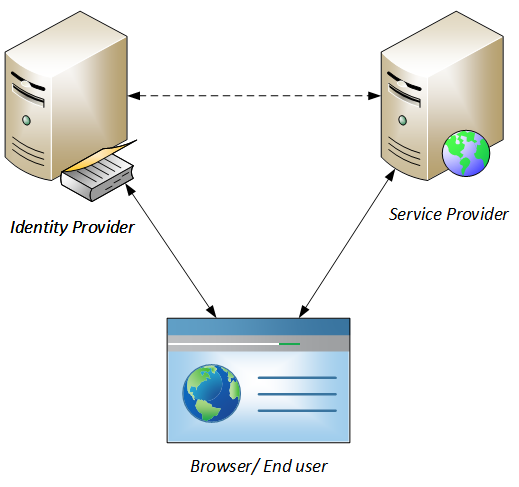
\includegraphics[scale=0.70]{graphics/Implementasjon/AutheticationFlow.png}}
    \caption{Skisse for illustrasjon av autentiseringflyt}
    \label{fig:authenticationFlow}
\end{figure}

\subsection*{SAML}
SAML\ref{sec:teoridel_SAML} omtales først og fremst som en autentisering protokoll og det er dette protokollen blir brukt til i Azure AD\cite{AadSamlSingelSignIn}. Autentiseringsflyten i protokollen er beskrevet overordnet i listen nedenfor, se figur \ref{fig:authenticationFlow}, og kan brukes for å enklere se sammenknytningen mellom sluttbruker, identity provider og applikasjon.
\\
\begin{itemize}
\item En sluttbruker (brukeren) spør en applikasjon om tilgang til beskyttede ressurser og applikasjonen håndterer ikke autentisering selv så sluttbrukeren blir sendt videre til en identity provider (Azure AD). 
\item Første gang brukeren skal logge på applikasjonen har ikke brukeren sesjonsdata som kan bevise at den er autentisert. Brukeren må derfor autentisere seg og vil bli sendt til en innloggingside. Når brukeren forsøker å logge inn på denne siden sendes forespørselen som en SAML forespørsel sammen med en "RelayState". "RelayState" er adressen brukeren skal sende tilbake dersom autentiseringen godtas. 
\item Brukerens nettleser mottar svar fra Identity Provideren ved vellykket innlogging og responsen kan sees på som en identifikasjonskode i form av en signatur. Denne signaturen lagres og videresendes til "RelayState" adressen. RelayState adressen er knyttet til applikasjonen brukeren ønsker å autentiseres for og er der brukeren må sende signaturen.
\item Applikasjonen mottar forespørselen om å åpne "RelayState" adressen sammen med SAML signaturen. Om applikasjonen godkjenner signaturen vil applikasjonen fullføre innloggingen og gi brukeren tilgang til de beskyttede ressursene.
\end{itemize}

\subsection*{OpenID Connect}
OAuth2 er mer en authorisasjonprotokoll enn en autentiseringprotokoll. OpenID Connect bygger videre på OAuth2 og fyller noen av manglene OAuth hadde. For å forklare OpenID Connect på en enkel måte må vi forklare litt rundt tokens. Mens SAML i prinsippet er basert på en etterprøvbar signatur, så baserer OpenID Connect seg på flere tokens. "Access token", "Refresh token" og "Identity token" brukes av OAuth og OpenID Connect, i tillegg benyttes en "Autentication code". I listen nedenfor blir autentiseringsflowen og bruken av tokens forklart på en forenklet måte. 

\begin{itemize}
\item En sluttbruker (brukeren) spør en applikasjon om tilgang til beskyttede ressurser. Applikasjonen håndterer ikke autentisering selv så sluttbrukeren blir sendt videre til en Identity provider (azure ad). 
\item Første gang brukeren logger på har ikke brukeren sesjonsdata lagret. Brukeren må autentisere seg og blir da sendt til en innloggingside. Etter autentiseringen mottar sluttbruker en authentiseringkode og en "redirect url". 
\item Autentiseringkoden har kort levetid. Den sendes via sluttbruker til en applikasjonsserver for å få en Access token. 
\item Applikasjonsserveren mottar forespørselen med autentiseringskoden og sender denne koden videre til Identity provideren. 
\item Identity provideren ser at tokenet er det samme som det som ble sendt til brukeren og svarer med å sende applikasjonsserveren et Access token tilbake.
\item Applikasjonsserveren sender bruker tokenet for å låse opp beskyttet data og sender både data og Access tokenet tilbake til sluttbrukeren.
\item Når brukeren skal spørre etter nye beskyttede data sender brukeren forespørsel til applikasjonsserveren med Access token.
\end{itemize}

I tillegg til Access token og autentiseringkode kan sluttbruker spørre en autentiseringsserver om to typer tokens til:
\begin{itemize}
\item Refresh token kan brukes for å få nye Access tokens uten å måtte oppgi på nytt både brukernavn og passord. Tokenet kan bli gitt av en autorisasjonserver og vil ha evig varighet. Dette betyr at så lenge brukeren ikke trekker tilbake tilgangen til en applikasjon eller logger ut så vil brukeren alltid være logget inn på applikasjonen. Refresh token kan mottas samtidig med Access tokene eller spørres etter separat.
\item Identity token er en samling av personlige data brukeren kan etterspørre fra Identity provideren. Det er designet slik at det kan etterprøves om dataene stemmer.
\end{itemize}

OpenID Connect og OAuth er bassert på JWT(JSON Web Token), mens SAML er bassert på XML (Extensible Markup Language).

\subsection{Logg ut}
\label{subsec:konfigurasjon_innloggingsmekanismer_loggUt}
For at Single Sign Out skal virke må Identity provideren vite om alle pågående autentiserte applikasjoner for hver bruker, samt kjenne til eller få beskjed om "LogoutURL". SAML og OAuth løser dette på nesten samme måte, med unntak av at pakkene som sendes er i ulike formater og med litt ulikt innhold. Applikasjoner som ikke er koblet til Identity provideren når utlogging pågår vil få en feilmelding nestegang brukeren tar de i bruk. Brukeren vil bli bedt om å logge inn igjen på nytt.

\begin{itemize}
\item Sluttbruker sender en forespørsel til en applikasjon om å logge ut av sin konto. Dette kan gjøres ved å klikke på en logg ut knapp.
\item Applikasjonen sender en "LogoutRequest", en utloggingsforespørsel, til Identitiy provideren via sluttbruker. 
\item Identity provideren logger ut brukeren og sender en "broadcast" melding til alle applikasjoner tilknyttet den autentiserte sesjonen og som identity provideren er tilknyttet.
\item Identity provideren sender en "LogoutRespons" tilbake til applikasjonen via sluttbruker og denne responsen inneholder en logg ut url. 
\item Applikasjonen ser responsen fra Identity provideren og fullfører utloggingen.
\end{itemize}

\subsection{Glemt passord}
\label{subsec:konfigurasjon_innloggingsmekanismer_glemtPassord}
Om en bruker har glemt passordet sitt til NorkartID kan brukeren trykke på lenken "Får du ikke tilgang til kontoen?" som ligger på innloggingsiden. Dette gjelder innloggingsiden levert av AAD, og brukes hver gang en bruker skal logge på en applikasjon enten det er en webapplikasjon (se implementasjonsbeskrivelse \ref{subsec:konfigurasjon_handteringAvApplikasjoner_leggTilApplikasjonIAzureAD}) eller en Android applikasjon ( se implementasjonsbeskrivelse \ref{subsec:konfigurasjon_handteringAvApplikasjoner_leggetilNyApplikasjon_androidApplikasjon}). Når denne linken blir trykket på vil brukeren bli sendt til AAD sin side for tilbakestilling av passord. Her vises en CAPTCHA test som bruker må fylle inn for å bevise at brukeren ikke er en robot. Når CAPTCHA testen er bestått, blir brukeren bedt om å velge hvilken autentiseringsmetode brukeren ønsker bruke å resette passordet. Disse alternativene må brukeren selv ha forhåndsdefinert ved et tidligere tidspunkt (se \ref{subsec:konfigurasjon_genrellHaandteringAvAad_tilbakestillingAvPassord} for konfigurasjonsbeskrivelser). Alternativene brukeren konfigurere er enten å svare på sikkerhetsspørsmål eller velge å motta en bekreftelseskode på ekstern e-post, sms eller via telefonsamtale. Under konfigurasjon kan bruker velge å registrere alle alternativene som mulige autentiseringsmekanismer eller bare en. Etter at den ekstra autentiseringsmekanismen er valgt og godkjent kan det skrives inn et nytt passord. Dette nye passordet kan deretter brukes for å logge inn på den ønskede nettsiden.\\
\\
Alle brukere må ha registrert autentiseringsdata for å bruke glemt passord funksjonaliteten. Dette kan gjøres på flere måter, enten via en registreringsportal, levert av Microsoft, eller ved pålogging på MyApps. Om ekstra autentiseringsmekanismer ikke er registrert vil MyApps spørre brukeren om å registrere dette. Registreringsportalen nås enten ved å gå direkte til \url{http://aka.ms/ssprsetup} eller via brukerportalen. Brukere kan logge seg inn i brukerportalen og trykke på "Registrer for tilbakestilling av passord". Begge metodene fungerer også om man har registrert bare noen av autentiseringsmetodene og ønsker å legge til fler, eller oppdatere eksisterende autentiseringsmetoder.
\\
\\
I registreringsportalen vil brukeren få valget om å registrere en ekstern e-post adresse, telefonnummer eller svare på sikkerhetsspørsmål. Dette avhenger av hvilke autentiseringsmetoder som er konfigurert i AAD av administratorene på forhånd. Ved registrering av ekstern e-post adresse vil brukeren motta en e-post med en verifiseringskode. Ved registrering av telefon gis valget mellom å få verifiseringskode på sms eller via telefonsamtale. Hvis sikkerhetsspørsmål er satt som autentiseringsmetode i AAD må det svares på et gitt antall sikkerhetsspørsmål.

\section{Egenadministrasjon}
\label{sec:konfigurasjon_egenadministrasjon}
Via myapps, den ferdig utviklede egenadministrasjon løsningen fra Microsoft kan man kun endre på grupperelasjoner og kjøre eventuelle applikasjoner man har tilgang til. For å kunne endre det som er nevnt i kravspesifikasjonen må det tas i bruk en egen løsning hvor man tar i bruk Windows PowerShell eller Graph API. Ved hjelp av disse tjenestene kan man gjøre det som er beskrevet i \ref{subsec:kravspesifikasjon_funksjonelleKrav_hoyNivaa}. Ved å implementere en egen brukerprofil nettside vil man kunne endre på e-post adressen, passord, mobil nummer og en rekke andre. Dette gjøres ved å bruke enten PowerShell eller Graph API og har sine restriksjoner med hva du kan endre på. Dette kan man ikke endre på men man kan endre på alle felter som er mulig å endre inne i selve Azure portalen. Passord resett kan gjøres ved å bruke myapps eventuelt ved å implementere det eksempelvis i en nettside eller applikasjon. Lager man en egen nettside klarer man å møte alle de sikkerhetskravene som er nevnt i kravspesifikasjonen.

\subsection{Endre brukerdata}
\label{subsec:konfigurasjon_egenadministrasjon_endreBrukerdata}
For å endre på brukerdata må dette gjøres utelukkende igjennom enten Graph API eller PowerShell. Hvis man logger inn på myapps for å se over sin konto samt sine tilganger til applikasjoner får man kun en oversikt over hva som er registrert på sin konto. For å endre dette må dette gjøres igjennom å lage en egen nettside eller applikasjon som endrer på disse dataene igjennom nevnte tjenester og API'er.

\subsection{Endre passord}
\label{subsec:konfigurasjon_egenadministrasjon_endrePassord}
Sluttbruker skal ha mulighet til å endre sitt eget passord. Dette er for å lette arbeidsmengden ytterligere hos kundeservice. For å gjøre dette trengs det å ha Azure Premium eller Basic, se lisensiering \ref{subsec:konfigurasjon_genrellHaandteringAvAad_lisensmodell}. Sluttbrukere kan endre sitt passord via brukeradministrasjonssiden myapps. Ved å trykke på "endre passord" i myapps må først gammelt passord oppgis. Deretter må nytt passord tastes inn to ganger og AAD har en rekke sikkerhetskrav til det nye passordet. {\color{blue} Bør vi skrive hvilke?}

\section{Brukeradministrasjon}
\label{sec:konfigurasjon_brukeradministrasjon}
Myapps fra Azure kan håndtere passord og forespørsler om grupper. Man kan gi gruppeansvar til en bruker i en gruppe og kan dermed håndtere hvilke entiteter som kan være med. Dette kan være andre brukere som forespør om de kan være med i gruppe. Myapps har ikke mulighet for å endre på informasjon knyttet til brukerne. Administreringen av flere brukere i en gruppe og kunne se samt endre på informasjon i henhold til kravspesifikasjon, beskrevet under \ref{subsec:kravspesifikasjon_funksjonelleKrav_hoyNivaa}, er mulig å oppnå ved bruk av Graph API eller PowerShell. Dette kan settes opp som en egen nettside vedsiden av Azure, eventuelt i Azure. Det kan også legges inn i applikasjoner, eksempelvis skrevet i C\#, som kan utvikles for å gjøre de ulike oppgavene som er ønsket mot brukerne. Legg til og fjerne brukere blir også håndtert av PowerShell eller Graph API. 

\section{Håndtering av brukere, roller og grupper}
\label{sec:konfigurasjon_handteringAvRollerOgGrupper}
I dette delkapitlet skal vi ta for oss ulike vurderinger og hvordan man skal gå fram for å få brukere og grupper inn i Azure.

\subsection{Masse-registrering av brukere}
\label{subsec:konfigurasjon_handteringAvRollerOgGrupper_masseRegistrering}
For å gjennomføre en masse-registrering av brukere er det flere alternativer som kan brukes for oppnå dette. Mulighetene man har er:
\begin{itemize}
\item Azure AD Sync
\item Graph API
\item PowerShell
\end{itemize}

Azure AD Sync på lokale AD'er er brukt for å synkronisere inn brukere fra lokale AD'er. Den muliggjør også å synkronisere inn multi-forests\footnote{En forest er en singel instanse av Active Directory. Multi-forests er en rekke Active Directories.} inn til AAD. Den kjører en stor initiell synkronisering hvor det sendes hele kontoer fra den lokale AD'en inn til Azure AD. Etter dette kjøres det et 3 timers intervall for å sjekke at alt er synkronisert. Dette kan endres til hvilket som helst intervall man ønsker. I tillegg til det kan man velge hvilke kontoer som skal synkroniseres ut i fra hvilken OU\footnote{OU, Organizational units, er AD sin beholder hvor man kan plassere brukere, grupper, datamaskiner og andre tjenester i organisasjonen og kan ikke inneholde objekter fra andre AD'er. Typisk brukt for å skille på brukere med samme navn} de ligger i. Ved å bruke Azure AD Sync kan du også sette på valgfrie funksjoner som  Eksempelvis "password writeback" for å synke passord tilbake til en lokal AD. Dette forsikrer deg om at endringer i passord blir skrevet tilbake til lokal AD og dermed kan dette brukes for å endre, eventuelt resette passord, gjennom Azure sine tjenester. Et resultat av dette er at brukere kan få tilgang til lokale datamaskiner som er administrert av en lokal AD ved å gå gjennom Azure tjenestene på Internett. Disse tjenestene er tilgjengelig hvor enn man er. \\
\\
Når du synkroniserer fra en eksisterende AD vil man kunne se dette på oversikten over brukere. Det vil stå "cloud" på de brukerne som ikke er i en lokal AD og det vil stå "Synced with Active Directory" for de som er både i skyen og i den lokale AD'en. De som ligger begge steder må først slettes i den lokale AD'en, for så å vente på at replikering kjøres mellom lokal AD og Azure AD, før de slettes i skyen. Man kan også importere brukere fra SQL databaser inn i Azure SQL. Ønsker man å få disse over i AAD må man gjøre dette gjennom PowerShell\footnote{Windows PowerShell er et rammeverk for konfigurasjonshåndtering og oppgave automatisering fra Microsoft som består av en kommandolinje basert skallprogram og har et skripte språk som er basert på .NET Framework.}. \\
\\
SQL databaser gjøres primært gjennom PowerShell skripting da formatet på dataen man henter ut varierer. Ved å bruke PowerShell kan man håndtere importen slik man ønsker og man har kontroll over hele prosessen. I kombinasjon med PowerShell kan man gjøre en masse registrering ved å bruke en liste av eposter hvor man ber hver og en om å gå inn for å registrere seg inn i systemet selv.

\subsection{Enkelt-registrering av brukere}
\label{subsec:konfigurasjon_handteringAvRollerOgGrupper_enkeltRegistrering}
{\color{blue} Skrive om at man kan registrere brukere direkte i Azure portalen også?}\\
For å registrere brukere kan man bruke Graph API for å lage en registreringside der man knytter seg til en Azure AD. Her kan man spørre om det man måtte trenge av detaljer og sende dette inn til AAD ved hjelp av Graph API. Ved siden av dette kan man registrere seg igjennom Azure portalen direkte også. Dette kan deretter bli knyttet til de grupper og roller man måtte ha i sin organisasjon.

\subsection{Håndtering av brukere}
\label{subsec::konfigurasjon_handteringAvRollerOgGrupper_haandteringAvBrukere}
{\color{blue} Skjønte ikke denne helt}\\
Et hendelsesforløp for brukere ville vært at når de registreres i AAD får de tildelt et midlertidig passord. Dette passordet kan man tvinge at skal endres ved første gangs innlogging. Dette medfører at brukeren blir kjent litt med hva som skjer i prosessen og kommer inn i Azure på mer eller mindre egne premisser. Siden myapps siden kommer til å være i Azure, eller om Norkart lager den selv, så er det viktig å kjenne til hvor man må gå for å nå NorkartID. NorkartID kan være en samle side for nyregistreringer, tilgang til brukerprofil og se eventuelt se tilstand i systemet med tanke på oppetid.

\subsection{Registrering av grupper}
\label{subsec::konfigurasjon_handteringAvRollerOgGrupper_grupper}
{\color{blue}Slå sammen registrering og håndtering av grupper?}\\
Ved hjelp av portalen kan man opprette de grupper man ønsker og legge inn medlemmene man vil ha i de respektive gruppene. Man har tilgang til det man måtte trenge for å opprette grupper og legge grupper inn i andre grupper. 
Powershell kan også nyttes for å opprette og håndtere grupper. 

\subsection{Håndtering av grupper}
\label{subsec::konfigurasjon_handteringAvRollerOgGrupper_grupper}
En gruppe i Azure er en samling av brukere og grupper som kan håndteres som en singel enhet. Brukere og grupper som tilhører en spesifikk gruppe vil bli omtalt som et gruppemedlem. Ved bruk av grupper kan man forenkle administreringen ved å tildele et standard sett med rettigheter og tilganger til en spesifikk gruppe. En bruker kan dermed legges inn i denne gruppen og få tilgangene og rettighetene til gruppen. I skrivende stund kan du kun lage sikkerhetsgrupper i Azure. Dette brukes for å tildele brukere tilgang til applikasjoner på gruppenivå. Ved å legge tilgang til en applikasjon mot en gruppe gjør dette det mulig å legge brukere inn i gruppen etterpå. Dette gjelder også når du håndterer tilganger til andre online tjenester. Handlinger du kan gjøre angående grupper i AAD:

\begin{itemize}
\item Lag en gruppe
\item Legg til et medlem i en gruppe
\item Fjerne et medlem i en gruppe
\item Endre en gruppes egenskaper
\item Slette en gruppe
\item Redigere gruppe eiere
\item Se rapport for gruppe aktivitet
\item Selvadministrer gruppe håndtering for brukere
\item Tildele tilgang for en gruppe til en SaaS applikasjon
\item Opprette dedikerte grupper
\item Opprette dynamisk medlemskap for grupper
\end{itemize}

\subsection*{Dynamiske Grupper}
AAD har en funksjonalitet de kaller dynamiske grupper. Dette er grupper som legger til medlemmer automatisk basert på hvilke attributter, som land eller avdeling, brukeren registrerer. Dette fører til at man da ikke går inn spesifikt for å legge en nyansatt utvikler i utviklergruppen fordi en merker av den nyansatte som utvikler, eller registrere hvilke avdeling, og AAD ordner tilgangen automatisk.

\subsection*{Gruppe Claims}
Gruppe claims gjør det lettere for skreddersydde applikasjoner å støtte deling grupper{\color{blue} ?} med andre brukere på tvers av en organisasjon. Denne typen applikasjon kan bruke gruppeinformasjon i AAD tokens for å gjøre det enklere for brukere å dele tilgang med andre brukere i organisasjonens AD. Dette forenkler deling og tilgangshåndtering ved å eliminere behovet for å håndtere gruppemedlemskap i flere applikasjoner. \cite{AppRoleOgClaims} \\
\\
Skisse over gruppeinndelingen hos oppdragsgiver tar vi ikke for oss i denne oppgaven, da vi antar oppdragsgiver ønsker å ta i bruk egne erfaringer med tidligere AD bruk i sin kommende AAD løsning. Oppdelingen av disse gruppene kan eksempelvis gjøres ved at man har grupper som representerer leserettigheter på en applikasjon, mens en annen grupper gir både lese og skriverettigheter på en applikasjon. Azure løser dette i henhold til administreringskravene satt i kravspesifikasjonen \ref{subsec:kravspesifikasjon_funksjonelleKrav_hoyNivaa}.

\subsection{Håndtering av roller}
\label{subsec::konfigurasjon_handteringAvRollerOgGrupper_roller}
Roller i Azure er et sett med handlinger som kan gjøres mot en Azure ressurs. En bruker kan utføre en handling på en Azure ressurs hvis de har blitt tildelt en rolle som inneholder denne handlingen. Azure har en rekke innebygde roller hvor hver av dem kan utføre ulike handlinger. Det er også mulighet for å opprette sine egne roller og tildele handlingene man ønsker. En rolle kan også tildeles til en tjeneste og vil kunne utføre det samme som en bruker. Roller kan du tildele til brukere, grupper eller tjenester. De rollene som Norkart trenger for å møte kravspesifikasjonen er \\
\begin{itemize}
\item Super administrator
\item Kundestøtte bruker
\item Lokal administrator
\item Sluttbruker
\end{itemize}
I Azure er det disse alternativene for brukere
\begin{itemize}
\item Billing administrator håndterer kjøpene, avtaler, tjenesteforespørsler  og overvåker tilstanden til tjenester.
\item Global administrator har tilgang til alle administrative tjenester og det kan kun være en i en organisasjon. Dette er den som skriver seg opp som Azure kontoholder. Det er kun denne rolle som kan tildele andre brukere administrator roller.
\item Password administrator resette passord, håndtere tjeneste forespørsler, og overvåker tjeneste tilstand. Man kan også resette passord bare for brukere og andre password administrators.
\item Service administrator håndtere tjenesteforespørsler og overvåker tilstanden til tjenstene.
\item User administrator resette passord, overvåker tjeneste tilstand og håndterer bruker kontoer, bruker grupper og tjeneste forespørsler. Det er noen begrensninger her, for eksempel kan kan ikke disse slette global administratoren eller lage andre administratorer. I tillegg kan de ikke resette passord for billing, global eller service administratorer.
\end{itemize}

Super administrator vil her være Service administrator. Kundestøtte bruker er User administrator og Lokal administrator er User administrator. Slutt bruker ville vært en user da det ikke er behov for administrator rettigheter på ordinære sluttbrukere.

\subsection*{Applikasjons rolle}
Dette muliggjør for utviklere til å deklarere et sett med roller i Azure AD som en applikasjon trenger for å autentisere. Brukere får tildelt roller og i innloggingøyeblikket avgjøre Azure AD hvilken rolle en bruker har og inkluderer dette i tokenet. Applikasjoner kan inspisere dette tokenet og bruke rollen som står for å autentisere bruker. Dette kan brukes for å si hvem som har tilgang til hvilken applikasjon og dette kommer til å være lagret på en sentral lokasjon, i Azure AD. \cite{AppRoleOgClaims}

\section{Håndtering av applikasjoner}
\label{sec:konfigurasjon_handteringAvApplikasjoner}
Denne seksjonen forklarer hva Norkart må ta hensyn til angående applikasjoner som skal benytte seg av AAD som en autentisering- og  autoriseringløsning. Applikasjonene må være registrert i en AAD og kan registreres og konfigureres i Azure portalen. I tillegg må det implementeres litt logikk i applikasjonene.

\subsection{Registrere applikasjon}
\label{subsec:konfigurasjon_handteringAvApplikasjoner_leggTilApplikasjonIAzureAD}
For at AAD skal klare å kommunisere med applikasjonene og vite hvilke rettigheter de har så trengs det en del informasjon. Hva slags informasjon og hvorfor den trengs \cite{RegistrereApplikasjoneriAAD} står beskrevet her:
\bigskip
\begin{description}
    \item [Applikasjons URI] \hfill \\ 
    Applikasjons URI er identifikatoren til en applikasjon. URI'en blir brukt når en bruker skal autentiseres for applikasjonen. Den blir sendt til AAD og forteller at det er denne applikasjonen brukeren ønsker token til. URI'en er i tillegg inkludert i tokenet, slik at applikasjonen vet at det var til seg brukeren ville. 
    \bigskip
    \item [Reply URL og redirect URL] \hfill \\
    Dette er URL'er AAD sender autentiseringrespons og token til, dersom autentisering lykkes. 
    \bigskip
    \item[Klient id og nøkkel] \hfill \\
    Klient id blir generert av AAD når applikasjonen registreres og er applikasjonens id. Denne brukes sammen med en nøkkel(client secret) når applikasjonen trenger tilgang til AAD gjennom Graph API eller andre API'er. Applikasjonen bruker nøkkelen og klient id for å be om Access token fra AAD OAuth 2.0 token endpoint. Token endpoint bruker da klient id og nøkkel til å autentisere applikasjonen før den sender ut et Access token.
\end{description} 
\bigskip

Applikasjoner i en AAD kan være kategorisert som enten single tenant eller multi tenant. Dette vil si om applikasjonene skal kunne kobles til flere AAD eller om alle brukerene av applikasjonen må ligge i samme AAD for hver enkelt installasjon av applikasjonen. Multi-tenant applikasjoner er som regel SaaS funksjoner. Nærmere forklaring om single tenant og multi tenant applikasjoner kan finnes i teori kapittelet under \ref{sec:singleTenantApplikasjon} og \ref{sec:multiTenantApplikajson}. For veiledning til hvordan applikasjoner kan registreres i en AAD, se brukerveiledning for dette i seksjon \ref{subsec:veiledninger_brukerveiledningForWebApplikasjon_registreringAvWebApplikasjoneriAad}, i kapittelet \ref{chap:veiledninger} \refname{chap:veiledninger}. Veiledningene viser registrering av single tenant applikasjoner. Konfigurering av multi-tenant applikasjoner blir ikke diskutert i denne oppgaven ettersom oppdragsgiver ikke har behov for dette. \ref{subsec:konfigurasjon_handteringAvApplikasjoner_konfigurereApplikasjonIAzureAD} \\

\subsection{Konfigurere applikasjon}
\label{subsec:konfigurasjon_handteringAvApplikasjoner_konfigurereApplikasjonIAzureAD}
Applikasjoner som er registrert i en AAD kan konfigureres i Azure portalen. Her kan applikasjonens tilgang til andre applikasjoner og web API'er settes, applikasjonsdata som URL, APP ID URI og logo kan endres samt brukerens adgang kan bestemmes. Denne seksjonen forklarer hvordan en single-tenant applikasjon kan gjøres om til å være multi-tenant, hvordan eksponere et web API, hvordan applikasjonen får tilgang til Graph API og hvilke regler som kan settes for brukeradgang til applikasjonen. Denne seksjonen er basert på Microsoft sine forklaringer rundt håndtering av applikasjoner i en AAD. \cite{AddingUpdatingRemovingApplications}

\subsection*{Konfigurere multi-tenant applikasjoner}
For å gjøre en single-tenant applikasjon om til en multi-tenant applikasjon må dette aktiveres under applikasjonens konfigurasjonsfane. Sett "Application is multi-tenant" til yes og lagre. Mulit-tenant applikasjoner må ligge både i bedriftens AAD og i alle AAD som har brukere som skal benytte seg av applikasjonen. Brukerne vil da få se hvilke rettigheter applikasjonen har og godkjenne disse. Når dette gjøres for native applikasjoner er det kun web API'et som ligger i brukernes AAD. 

\subsection*{Web API}
Hvis oppdragsgiver ønsker å eksponere et web API til andre applikasjoner i AAD kan dette gjøres ved å laste ned manifestet til API'et og endre OAuth 2.0 rettighetene. Manifestet kan lastes ned ved å trykke på "Manage manifest" i bunnmenyen. Bytt ut innholdet i JSON manifestet til:

\begin{lstlisting}[caption={JSON manifest},label={lst:JSON_manifest}]
   "oauth2Permissions": [
    {
      "adminConsentDescription": "Allow the application full access to the Todo List service on behalf of the signed-in user",
      "adminConsentDisplayName": "Have full access to the Todo List service",
      "id": "b69ee3c9-c40d-4f2a-ac80-961cd1534e40",
      "isEnabled": true,
      "origin": "Application"
      "type": "User",
      "userConsentDescription": "Allow the application full access to the todo 
      service on your behalf",
      "userConsentDisplayName": "Have full access to the todo service",
      "value": "user_impersonation"
    }
  ],
\end{lstlisting}

Bytt ut teksten til å passe API'et. Id'en er en unik identifikator for rettighetene som gis av API'et og denne må være en GUID. Last så opp det nye manifestet i Azure portalen. Web API'et vil nå være tilgjengelig for andre applikasjoner.

\subsection*{Få tilgang til Graph API}
Hvis applikasjoner trenger tilgang til Graph API kan dette konfigureres under "permissions to other applications". Tilgang til Graph API, er satt som standardinnstilling for alle applikasjoner i AAD og kalles Windows Azure Active Directory. Tilgangen applikasjonen trenger fra Graph API, som lese og skrive rettigheter eller kun lese rettigheter kan også settes her. 

\subsection*{Adgangsregler}
I AAD er det mulig å sette en del adgangsregler for hvilke brukere som skal ha adgang til applikasjonen og hvordan. Denne funksjonaliteten er i skrivende stund kun tilgjengelig som preview. Adgangsreglene for en applikasjon kan gjelde for alle brukere, spesifikke brukere eller spesifikke grupper. Så langt i Azure sitt livsløp er det kun mulig å sette regler for multifaktor autentisering. Det kan konfigureres om multifaktor autentisering alltid skal brukes eller at det kun skal brukes dersom brukere logger seg inn via usikre nettverk. Dette gjøres ved å sette hvilke nettverk som er trygge i Azure Portalen. Det er også mulig å la brukere utsette multifaktor autentisering ved å huske sine enheter i 1 - 60 dager. \\
\\
I følge Alex Simons, direktør for programledelse i Microsofts identitets og sikkerhetsdivisjon, vil det bli mulig å sette flere typer adgangsregler i fremtiden\cite{AccessRules}. Microsoft forklarer at det vil komme flere typer adgangsregler som kan settes i fremtiden, men sier ikke når.

\subsection{Implementering av Webapplikasjon - ASP.NET MVC}
\label{subsec:konfigurasjon_handteringAvApplikasjoner_Webapplikasjon}
Applikasjoner som skal bruke AAD som autentiseringsverktøy må implementere en del elementer. For webapplikasjoner må det blant annet legges inn noen biblioteker for å kunne benytte OIDC protokollen og litt informasjon som AAD trenger for å autentisere brukere opp mot applikasjonen. \\
\\
For at applikasjonen skal bruke AAD autentisering via OIDC protokollen må den være en OWIN basert applikasjon. Dette gjøres ved å installere Katana elementene OWIN system.web og OWIN security. Se \ref{lst:katana_elementer} OWIN security pakken gjør det mulig å velge OIDC som autentiseringsprotokoll. \cite{WebappTutorialCloudIdentity}

\begin{lstlisting}[caption={Katana elementer},label={lst:katana_elementer},numbers=left,escapeinside={@}{@}]
Install-Package Microsoft.Owin.Security.OpenIdConnect -Pre
Install-Package Microsoft.Owin.Security.Cookies -Pre
Install-Package Microsoft.Owin.Host.SystemWeb -Pre
\end{lstlisting}

\bigskip
I tillegg til Katana elementene må det implementeres litt logikk i applikasjonen. Det må lages klasser for å konfigurere autentisering og disse kommer til å bruke Owin mellomvaren og setter OIDC som autentiseringsprotokoll. I tillegg kan det her settes mange egenskaper for OIDC. For at OIDC protokollen skal fungere er det kun nødvendig å sette noen få egenskaper, se \ref{lst:satrtup_auth_cs}. Egenskapene som trengs er applikasjonens id i AAD (klient id), metadata som trengs for å motta nøkler fra AAD, altså innloggingsurl til AAD tenanten. URL som bruker skal sendes til, etter logg ut, kan også settes her. 

\begin{lstlisting}[caption={Startup.Auth.cs},label={lst:satrtup_auth_cs},numbers=left,escapeinside={@}{@}]
app.UseOpenIdConnectAuthentication(
    new OpenIdConnectAuthenticationOptions
    {
        ClientId = clientId,
        Authority = authority,
        PostLogoutRedirectUri = postLogoutRedirectUri
    });
\end{lstlisting}

\bigskip
I applikasjoner som ikke bruker innlogging fra før må det legges til et logg inn view som må refereres til i layout filen og en controller som behandler innlogging og utlogging. Slik får applikasjonen logg inn og logg ut knapper med funksjonalitet i hovedmenyen. Controlleren, se \ref{lst:account_controller_cs}, har ansvaret for å sende innloggings og utloggingsforespørsler til Owin og OIDC. 

\begin{lstlisting}[caption={AccountController.cs},label={lst:account_controller_cs}]
public class AccountController : Controller
{
    public void SignIn()
    {
        // Send an OpenID Connect sign-in request.
        if (!Request.IsAuthenticated)
        {
            HttpContext.GetOwinContext().Authentication.Challenge(
                new AuthenticationProperties { RedirectUri = "/" }, 
                OpenIdConnectAuthenticationDefaults.AuthenticationType);
        }
    }
    public void SignOut()
    {
        // Send an OpenID Connect sign-out request.
        HttpContext.GetOwinContext().Authentication.SignOut(
            OpenIdConnectAuthenticationDefaults.AuthenticationType, 
            CookieAuthenticationDefaults.AuthenticationType);
    }
}
\end{lstlisting}

\bigskip
For at AAD skal kunne autentisere brukere opp mot applikasjonen må det settes fire verdier i web.config filen under
<AppSettings>, se \ref{lst:web_config}. 

\begin{itemize}
    \item ClientId blir forklart nærmere under seksjonen Registrere applikasjoner i \ref{subsec:konfigurasjon_handteringAvApplikasjoner_Webapplikasjon}
    \item AADInstance vil si hvilken instanse av Azure som brukes. Her brukes https://login.windows.net/{0} som er den offentlige Azure AD instansen.
    \item Tenant er navnet, eller domene til den aktuelle  AAD tenanten. Dette kan være et domene gitt av Azure eller det kan være et eget domene som er registrert for den aktuelle AAD.
    \item PostLogoutRedirectUri er URL'en brukerne vil bli viderekoblet til etter utlogging
\end{itemize}

\begin{lstlisting}[caption={Web.config},label={lst:web_config}]
    <add key="ida:ClientId" value="1ef05302-c640-4459-a2b1-3c660c9854db" />
    <add key="ida:AADInstance" value="https://login.windows.net/{0}" />
    <add key="ida:Tenant" value="NorkartIDDevelopment.onmicrosoft.com" />
    <add key="ida:PostLogoutRedirectUri" value="https://norkartidman.azurewebsites.net/" />
\end{lstlisting}

\bigskip
For å sikre kommunikasjon mellom webapplikasjon og AAD er det viktig at SSL aktiveres i applikasjonen.

Kodeeksemplene presentert i denne seksjonen er i hovedsak hentet fra et kodeeksempel i GitHub under AzureAD Samples som heter WebApp-OpenIDConnect-DotNet \cite{WebAppOpenIDConnectDotNet}. Microsoft referer til dette kodeeksemplet flere steder på deres sider når det gjelder implemenetring av AAD som autentiseringsverktøy for webapplikasjoner.

\subsection{Implementering av Android-applikasjon}
\label{subsec:konfigurasjon_handteringAvApplikasjoner_leggetilNyApplikasjon_androidApplikasjon}
For å knytte Android applikasjoner til Azure for å bruke AAD som autentisering er det flere ting som må gjøres. Dette delkapitlet vil forklare overordnet hvilke elementer som må knyttes sammen og hvorfor, mens det i punkt \ref{sec:veiledninger_androidBrukerveliedning} er lagt ved en fullstendig brukerguide som viser hvordan dette kan gjøres ved bruk av en eksempelapplikasjon. \\
\\
\subsubsection{Mobile Services}
Mobile Services er en Azure tjeneste som gjør det enkelt å koble mobile applikasjoner mot en backend server med database, serverlogikk, autentisering og skalerbarhet. Vår eksempelapplikasjon tar utgangspunkt i en mobile-service backend for å teste lagring i en Azure database. Eksempelet ( se \ref{sec:veiledninger_androidBrukerveliedning}) viser litt bruk av backend logikk og programmering av ytterligere API kall. \\
\\
Norkart har applikasjoner og tjenester som bruker data fra flere større databaser. Her er det mulig å programmere applikasjoner som jobber direkte mot disse databasene, eller lage backend logikk som jobber mot eksterne databaser, for så å sende data fra eksterne databaser tilbake til brukerne igjennom azure mobile services.\\
\\
For å bruke Azure AD som autentisering for en applikasjon må man først opprette en applikasjon i Mobile Services, for deretter å knytte den til en Identity Provider. I tillegg kan det være hensiktsmessig å begrense rettighetene i databasen til kun autentiserte brukere.

\subsubsection{Azure Active Directory}
For alle typer applikasjoner som skal knyttes mot AAD må det opprettes en applikasjon i AAD. Denne applikasjonen må så knyttes mot applikasjonen opprettet i Mobile Services. Hvordan disse applikasjonene knyttes sammen gjøres ved hjelp av en applikasjons URL og en client ID, se gjerne brukerveiledningen i kapittel \ref{subsec:veiledninger_androidBrukerveliedning_del2-LeggInnAutentiseringIApplikasjonen} for en beskrivelse av hvordan dette gjøres. \\
\\
Etter det prosjektgruppen har funnet ut så må alle autorisasjonnivåer internt i en applikasjon håndteres av applikasjonens egen database og kode. Når AAD fungerer som Identity provider gir den kun tilgang eller ikke tilgang til selve applikasjonen. Men ettersom AAD støtter OpenID kan applikasjonen også få vite av AAD hvilken bruker som har fått tilgang og autorisasjon kan bygges utifra denne informasjonen. 

\subsubsection{Android kode}
Det å få en Android applikasjon til å fungerer hensiktsmessig i forhold til autentiseringsfunksjonalitet kreves det at hele applikasjonen skrives for å støtte autentisering. I eksempelapplikasjonen som bygges i brukerveiledningen i kapittel \ref{sec:veiledninger_androidBrukerveliedning} legges det inn autentisering for å åpne applikasjonen og dersom autentiseringsprosessen ikke blir vellykket avsluttes applikasjonen. Dette er ikke nødvendigvis den beste måten å implementere autentisering for alle applikasjoner. Brukerguiden viser likevel at det er få kodelinjer som skal legges til i Android for å bruke AAD som Identity provider for en applikasjon. Kodelinjene tar ibruk biblioteker som delvis bruker lokale funksjoner og delvis bruker webview mot AAD pålogging. Det er klare likheter mellom webviewet for innlogging fra en Androidapplikasjon og innlogging til en webapplikasjon fra en nettleser. Også i innloggingen i Android applikasjonen er det lagt inn branding ved hjelp av bedriftslogo og glemt-passord funksjonalitet.

\section{Generell konfigurasjon av AAD}
\label{sec:konfigurasjon_genrellHaandteringAvAad}
Konfigurasjon av Azure AD som en Identity Provider gir administrator mulighet til å endre og tilpasse på en rekke parametere. Det er blant annet mulig å konfigurere tilbakestilling av passord, generell forvaltning av grupper, applikasjons proxy og bruker adgang. Prosjektgruppen anser mye av innstillingene som kan settes som selvforklarende (se skjermbilde på figur \ref{fig:KonfigAvAzureAD}). Vi har derfor valgt og kun beskrive noen få av konfigurasjonsmulighetene nærmere.  

\begin{figure}[h]
    \centering
    \setlength{\fboxsep}{0pt}%
    \setlength{\fboxrule}{1pt}%
    \fbox{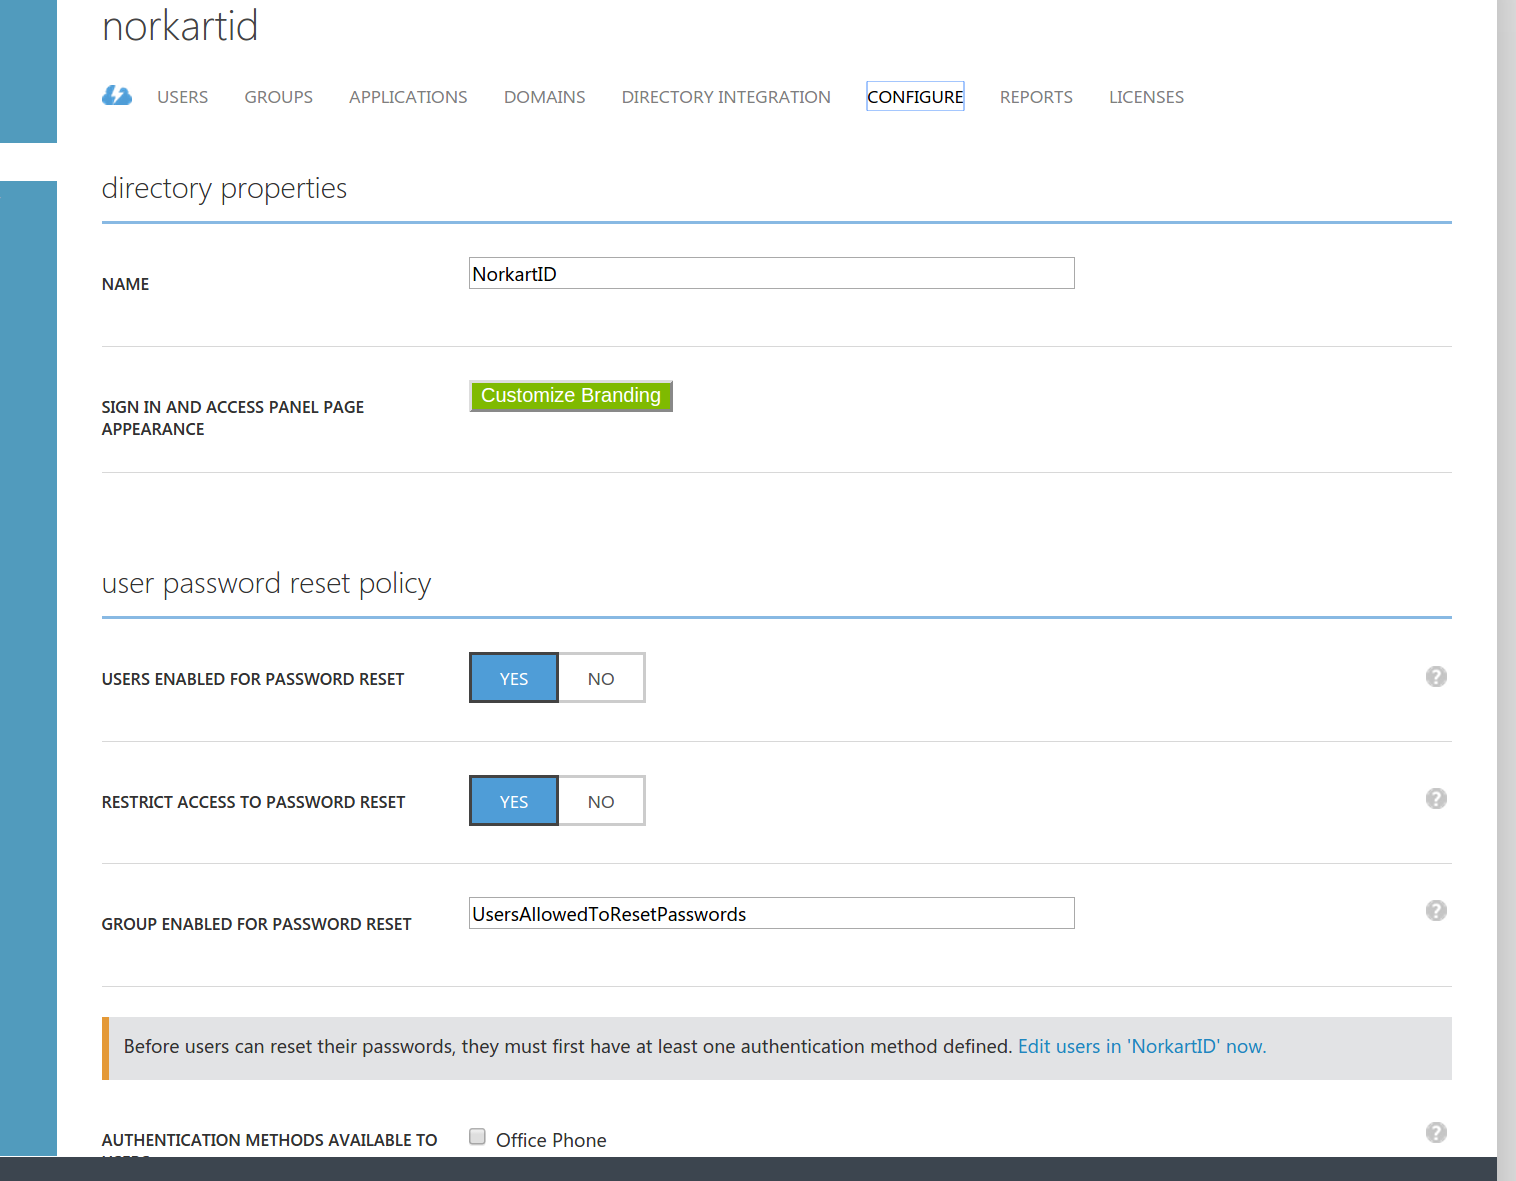
\includegraphics[scale=0.24]{graphics/Implementasjon/AzureADkonfigurasjon.png}}
    \caption{Generell overordnet konfigurasjon av Azure AD}
    \label{fig:KonfigAvAzureAD}
\end{figure}


\subsection{Lisensmodell}
\label{subsec:konfigurasjon_genrellHaandteringAvAad_lisensmodell}
Azure AD har en egen lisensieringsmodell i forhold til Azure tjenester. I skrivende stund (17 April 2015) er det ikke sluppet en offisiell B2C eller B2B tjeneste for AAD. Prosjektgruppen har vært i kontakt med Microsoft ansatte som ikke kan bekrefte eller avkrefte i forhold til hemmelighold, men som indikerer at denne funksjonaliteten vil slippes i nærmeste framtid. Om Norkart skulle basert seg på dagens lisensmodell vil brukere som knytter seg til NorkartID trolig måttet ha en Premium lisens for hver enkelt bruker. \\
\\
Lisensmodellen i Azure AD er lagt på hver enkelt bruker i brukerdatabasen \cite{AzureADPricing}. Første nivå kalles "Free" som er gratis for de første 500 000 brukerene. Andre nivå heter "basic" som det ikke finnes noen fast pris på, men må forhandles fram mellom bedriften og Mircosoft for hvert enkelt samarbeidsavtale. Siste nivået kalles "Premium" og lisensieres per bruker og koster i skrivende stund i underkant av 37 kr per bruker i måneden. Premium vil gi tilgang til det Azure AD har av funksjonalitet og tilby dette for hver eneste bruker. Muligheten til å endre passord selv, bruk av flerfaktor autentisering og mulighet for tilknytning til fler enn 10 applikasjoner per bruker er kun tilgjengelig for Premium brukere. Dette vil si at dersom Norkart har 1000 brukere de skal knytte til NorkartID igjennom Azure AD vil dette koste dem ca 37 000 kr i måneden, og ca 435 000 i året. Microsoft ønsker ikke å si noe om lisensieringsmodellene for de nye tjenestene B2C og B2B, men indikasjoner tilsier at det vil bli litt rimeligere. Prosjektgruppen har ikke lykkes med å få noen annen bekreftelse enn hva Nasos Kladakis, "Product Marketing Manager" for Azure AD, sier under en konferanse i November 2014 \cite{NasosAzureADExplained} om at begge tjenestene slippes innen et år. Da prosjektgruppen tok kontakt direkte med Kladakis kunne han hverken bekrefte eller avkrefte hva som ville slippes, men kom med indikasjoner på at det ville skje noe under Microsoft Build\cite{MicrosoftBildConference} konferansen i slutten av April 2015.

\subsubsection{Tilbakestilling av passord}
\label{subsec:konfigurasjon_genrellHaandteringAvAad_tilbakestillingAvPassord}
{\color{blue} Skal dette være med?} \\
For at brukere skal kunne egenadministrere passord for sin konto må dette aktiveres under konfigurasjonsfanen til aktuell AAD i Azure portalen. Det kan settes at det kun er brukere i en spesifikk gruppe som skal kunne gjøre dette. Hvilke autentiseringsmetoder som skal brukes og hvor mange kan også konfigureres. Det kan velges opp til to autentiseringmetoder. Valgene her er å autentiseres via jobbtelefon, mobiltelefon, ekstern e-post adresse eller sikkerhetsspørsmål. Hvis sikkerhetsspørsmål velges er det mulig å konfigurere antall spørsmål, samt eksempler på spørsmål. \\
\\
Dette vil si alle brukere som skal kunne endre sitt eget passord må registrere gjeldene autentiseringssdata. For å sikre at brukere gjør dette kan det aktiveres at bruker må registrere autentiseringsdata neste gang brukeren logger inn i brukerportalen. Antall dager før neste gang bruker må kontrollere sin autentiseringsdata kan også konfigureres her. Hvis bruker møter på problemer når passord skal endres vises en "kontakt din administrator" lenke. Denne kan konfigureres og settes til en spesifikk e-post adresse eller en URL. Hvis dette ikke settes vil det sendes en e-post til maks hundre administratorer hvor bruker spør om å få resatt sitt passord.\\
\\
Under konfigurasjonsfanen i AAD ligger det en lenke til en registreringsportal for brukere. Denne linken fungerer i skrivende stund (13.04.2015) kun for Microsoft kontoer, den vil da ikke fungere for Norkart sine AAD brukere.
\chapter{Testing}
\label{chap:testing}
I dette delkapitlet kommer vi til å gjennomføre en del tester for å se om Azure tilfredsstiller de operasjonelle kravene definert i denne oppgaven. Det vil kjøres tester mot de høynivå use casene som er definert i kapittel \ref{subsec:kravspesifikasjon_funksjonelleKrav_hoyNivaa} \nameref{subsec:kravspesifikasjon_funksjonelleKrav_hoyNivaa} og det vil gjennomføres en brukeranalyse hvor vi tar for oss Azure som verktøy for Norkart. Avslutningen av dette kapitlet inneholder drøfting av resultater fra den gjennomførte testingen.

\subsection{Implementasjontesting}
\label{sec:testing_implementasjontesting}
Tester her funksjonelle krav \\
Testing av løsning \\

Intro\\
For å teste at de funksjonelle kravene til løsningen blir overholdt er det gjennomført funksjonstesting av AAD i Azure portalen og på demo applikasjonene gruppen har utviklet, altså web applikasjoner og en native applikasjon. Prosjektgruppen har utviklet testscenarier som kan gjennomføres uten å ha innsyn i koden, altså black box tester. Disse har til hensikt å teste at funksjonaliteten oppfyller kravene. Testene er utviklet på bakgrunn av høynivå use case beskrivelsene i kravspesifikasjonen, se \ref{subsec:kravspesifikasjon_funksjonelleKrav_hoyNivaa}.

\subsection{Innloggingsmekanismer}
\label{sec:testing_innloggingsmekanismer}
Testing \\
Hentet fra kravspek:
Aktør skal kunne logge seg inn og få sikker tilgang til ønsket applikasjon. Dette skal være SSO slik at aktør i tillegg blir autentisert for andre applikasjoner aktør har tilgang til. Aktør skal i tillegg kunne logge seg ut av en applikasjon. Det skal også være mulig for aktør å gjenopprette sitt eget passord dersom dette er glemt.


Resultater av testing \\

\subsection{Egenadministrasjon}
\label{sec:testing_egenadministrasjon}
Testing \\

Hentet fra kravspek:
Aktør skal selv kunne endre og registrere? på egne regist- rerte opplysninger på sin brukerprofil.

Resultater av testing \\

\subsection{Brukeradministrasjon}
\label{sec:testing_brukeradministrasjon}
Testing \\

Hentet fra kravspek:
Håndtere brukere innenfor en gitt gruppe.

Resultater av testing \\

\subsection{Håndtering av brukere, grupper og roller}
\label{sec:testing_haandteringAvBrukereGrupperOgRoller}
Testing \\

Hentet fra kravspek:
Aktør skal kunne registrere og håndtere brukere, grupper og roller.

Resultater av testing\\

\subsection{Håndtering av applikasjoner}
\label{sec:testing_handteringAvApplikasjoner}
Testing \\

Hentet fra kravspek:
Aktør skal kunne registrere og administrere applikasjoner i en AAD. I tillegg skal aktør kunne klargjøre applikasjoner for bruk av løsningen.

Resultater av testing \\

\subsection{Drøfting av resultat opp mot krasvpek}
\label{sec:testing_droftingAvResultatOppMotKrasvpek}
Drøfting av resultat opp mot kravspek

\section{Målbare tester mot kravspesifikasjon}
\label{sec:testing_malbareTesterMotKravspesifikasjon}
{\color{red}TODO}
Tester her operasjonelle krav \\
Da tenkte jeg at vi referer til Microsoft dokumentasjon.\\
\\
Intro \\

\subsection{Ytelse}
\label{sec:testing_malbareTesterMotKravspesifikasjon_ytelse}
Testing \\

Hentet fra kravspek:
• Løsningen skal som minimum takle 10 000 brukere innlogget samtidig.
• Løsningen skal håndtere pålogging av 100 brukere i minuttet.
• Løsningen skal bygges for å være skalerbar.

Resultater av testing \\

\subsection{Sikkerhet og Autentisering}
\label{sec:testing_malbareTesterMotKravspesifikasjon_sikkerhetOgAutentisering}
Testing \\
Resultater av testing \\

\subsection{Universell Utforming}
\label{sec:testing_malbareTesterMotKravspesifikasjon_universellUtforming}
Testing \\
Resultater av testing \\
\\

\subsection{Drøfting av resultat mot kravspek}
\label{sec:testing_droftingAvResultatMotKravspek}
Drøfting av resultat opp mot kravspek \\

\section{Brukervennelighetsanalyse}
\label{sec:testing_brukervennelighetsanalyse}
{\color{red}TODO}
Analyse av sluttbrukere \\
Analyse av kundeservice og administrator \\
Test av alle roller \\
Test logg inn, logg ut, resett passord og brukeradmin? \\
Hvilke krav skal disse basreres på? \\
Universell utforming/operasjonelle krav om brukervennlighet? \\

Intro\\
Det er viktig for oppdragsgiver at løsningen er brukervennlig for alle rollene som skal bruke den. "En brukervennlig løsning skal føre brukeren til målet på en effektiv og forståelig måte." \cite{Brukervennlighet} Analyse av brukervennlighet vil her baseres på at kravene til brukervennlighet i kravspesifikasjonen \ref{subsec:kravspesifikasjon_operasjonelleKrav_brukervennlighet} opprettholdes og at rollene får utført hovedfunksjonene beskrevet i høynivå use case beskrivelser \ref{subsec:kravspesifikasjon_funksjonelleKrav_hoyNivaa}.  
\\
For å analysere brukervennligheten er det først utført brukertester på systemet. Brukertester vil si å la brukere av løsningen få oppgaver som skal utføres samtidig som de blir observert. Resultatet av brukertestene kan så brukes til å evaluere løsningens brukervennlighet. \cite{PraktiskBrukertesting}


Testing \\
Analyse \\
Analyse / Drøfting av resultat opp mot kravspek \\

\section{Drøfting av testresultat for hele løsningen}
\label{sec:testing_drøftingAvResultat}

\chapter{Veiledninger}
\label{chap:veiledninger}
Dette kapittelet består av brukerveiledninger for implementering autentisering i webapplikasjon og android ved hjelp av Azure Active Directory.

\section{Brukerveiledning for web applikasjon}
\label{sec:veiledninger_brukerveiledningForWebApplikasjon}
Denne veiledningen viser hvordan en web applikasjon kan registreres i en AAD og hvordan AAD kan implementeres i en ASP.NET Web app laget i Visual Studio 2013. Autentisering er satt til "No Authentication".
\\
\\
Kodeeksemplene presentert i denne seksjonen er i hovedsak hentet fra et kodeeksempel i GitHub under AzureAD Samples som heter WebApp-OpenIDConnect-DotNet \cite{WebAppOpenIDConnectDotNet}. Microsoft referer til dette kodeeksemplet flere steder

\subsection{Registrering av web applikasjoner i AAD}
\label{subsec:veiledninger_brukerveiledningForWebApplikasjon_registreringAvWebApplikasjoneriAad}
For å kunne bruke AAD som autentiseringsverktøy må applikasjonene registreres i en AAD. Dette gjøres ved å logge inn i Azure portalen og navigere til aktuell AAD. Velg applikasjoner i topp menyen og trykk så på add i bunnmenyen. En dialogboks vil nå vises.
\\
\begin{enumerate}
\item Velg "Add an application my my organization is developing"
\\
\item Skriv inn navnet til applikasjonen. Dette blir navnet til applikasjonen i AAD. Velg web app/ web api og trykk på pilen for å gå videre
\\
\item Fyll inn sign-on url og App ID URI, se figur \ref{fig:registrereAppIAAD}. Sign-on url er base urlen til web applikasjonen eller web apiet. Her må https:// eller http:// være med i urlen. App ID URI er applikasjonen sin ID. Denne blir brukt når en bruker skal autentiseres for applikasjonen. App IDen blir sendt til AAD og forteller at det er denne applikasjonen brukeren ønsker token til. APP IDen er i tillegg inkludert i tokenet, slik at applikasjonen vet at det var til seg brukeren ville.
\pagebreak
\begin{figure}[!htbp]
\begin{center}
    {%
    \setlength{\fboxsep}{0pt}%
    \setlength{\fboxrule}{0.5pt}%
    \fbox{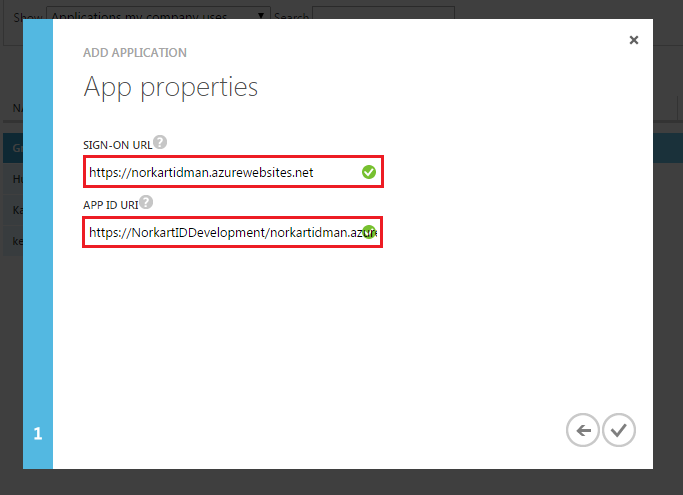
\includegraphics[scale=0.5]{graphics/veiledninger_implementereWebApp/regWebApp5}}%
    }%
    \caption{Registrere applikasjon i AAD}
    \label{fig:registrereAppIAAD}
    \end{center}
\end{figure}
\\
\item Klikk på ferdig. Nå er appikasjonen registrert i AAD og kan benyttes av brukere i AAD
\end{enumerate}


\subsection{Implementering av AAD i web applikasjon}
\label{subsec:veiledninger_brukerveiledningForWebApplikasjon_implementeringAvAADIWebApplikasjon}
For å kunne bruke AAD som autentiseringsverktøy for en web applikasjon må det legges til en del elementer i applikasjonen. Blandt annet må det legges inn noen biblioteker for å kunne benytte OpenID Connect protokollen og noe informasjon som AAD trenger for å autentisere brukere opp mot applikasjonen.

\subsection*{SSL}
SSL brukes for å sikre kommunikasjonen mellom applikasjonen og AAD. SSL kan aktiveres i Visual Studio. Se figur \ref{fig:aktiverSsl}
\\
\begin{enumerate}

  \item I solution explorer klikk på applikasjonen. da vises “properties” vinduet. Sett SSL-enabled til true og noter ned SSL URL.
    \begin{figure}[!htbp]
    \centering
        \begin{subfigure}{.3\textwidth}
            \centering
             {%
            \setlength{\fboxsep}{0pt}%
            \setlength{\fboxrule}{0.5pt}%
            \fbox{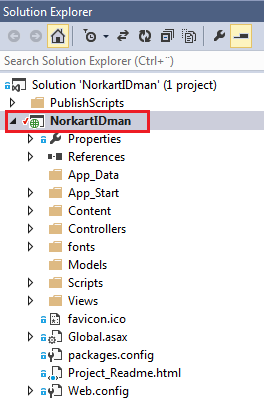
\includegraphics[scale=0.4]{graphics/veiledninger_implementereWebApp/impWebApp1_1}}%
            }%
            \label{fig:aktiverSsl1}
        \end{subfigure}%
        \begin{subfigure}{.5\textwidth}
            \centering
             {%
            \setlength{\fboxsep}{0pt}%
            \setlength{\fboxrule}{0.5pt}%
            \fbox{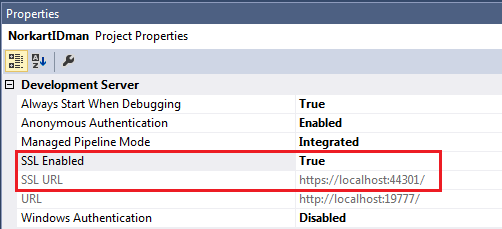
\includegraphics[scale=0.55]{graphics/veiledninger_implementereWebApp/impWebApp1_2}}%
            }%
            \label{fig:aktiverSsl2}
        \end{subfigure}
        \caption{Aktiver SSL}
        \label{fig:aktiverSsl}
    \end{figure}

  \item Høyreklikk på appikasjonen og velg properties. Velg web og endre “Project URL” til å SSL URL, se figur \ref{fig:aktiverSsl}.
  \pagebreak
    \begin{figure}[!htbp]
        \begin{center}
             {%
            \setlength{\fboxsep}{0pt}%
            \setlength{\fboxrule}{0.8pt}%
            \fbox{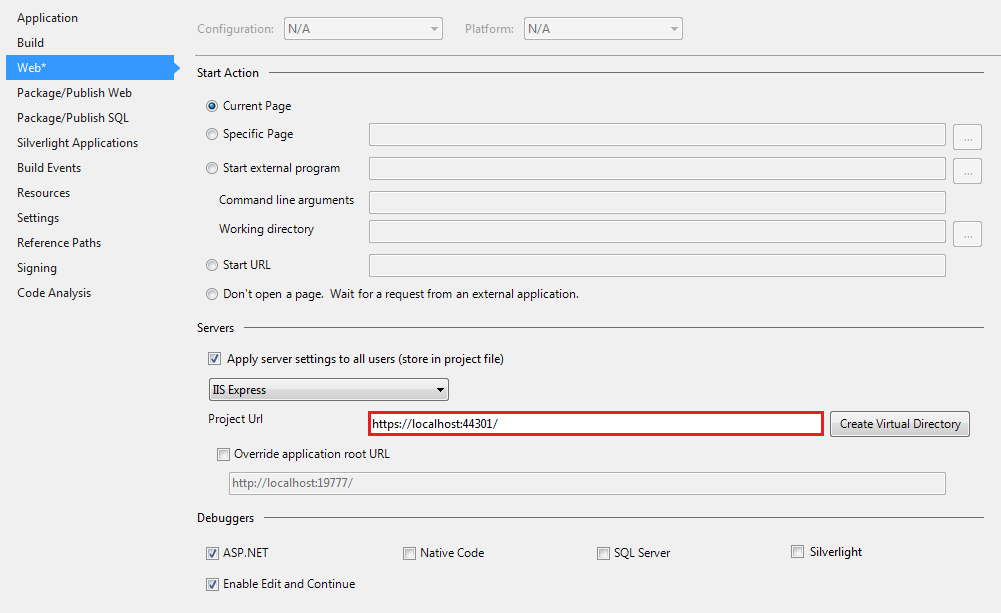
\includegraphics[scale=0.5]{graphics/veiledninger_implementereWebApp/impWebApp2}}%
            }%
            \caption{Registrer SSL url}
            \label{fig:registrerSslUrl}
        \end{center}
    \end{figure}
\end{enumerate}

\subsection*{Implementere OWIN pakker}

\begin{enumerate}
  \item For at AAD skal bruke OpenID Connect som autentiseringsprotokoll må det legges til noen biblioteker i applikasjonen. Åpne Nuget konsollen i Visual Studio og installer følgende Katana elementer, \ref{lst:katana_elementer}:
    \begin{lstlisting}[caption={Katanaelementer},label={lst:katana_elementer},numbers=left,escapeinside={@}{@}]
        Install-Package Microsoft.Owin.Security.OpenIdConnect -Pre
        Install-Package Microsoft.Owin.Security.Cookies -Pre
        Install-Package Microsoft.Owin.Host.SystemWeb -Pre
    \end{lstlisting}
\end{enumerate}

\subsection*{Implementere autentiseringslogikk}

\begin{enumerate}
\item Naviger til “App\_Start” mappen i prosjektet og legg til en C\# klasse som heter Startup.Auth.cs. Fjern App\_Start fra namespace og legg til referanser og kode i Startup.Auth.cs, se \ref{lst:startupAuth}. 
\begin{lstlisting}[captionpos=b, caption={Startup.Auth.cs},label={lst:startupAuth},numbers=left]
        using Owin;
using Microsoft.Owin.Security;
using Microsoft.Owin.Security.Cookies;
using Microsoft.Owin.Security.OpenIdConnect;
using System.Configuration;
using System.Globalization;
using System.Threading.Tasks;

namespace WebApp_OpenIDConnect_DotNet
{
    public partial class Startup
    {
        private static string clientId = 
            ConfigurationManager.AppSettings["ida:ClientId"];
        private static string aadInstance = 
            ConfigurationManager.AppSettings["ida:AADInstance"];
        private static string tenant = 
            ConfigurationManager.AppSettings["ida:Tenant"];
        private static string postLogoutRedirectUri
            ConfigurationManager.AppSettings["ida:PostLogoutRedirectUri"];

        string authority = 
        String.Format(CultureInfo.InvariantCulture, aadInstance, tenant);

        public void ConfigureAuth(IAppBuilder app)
        {
            app.SetDefaultSignInAsAuthenticationType(
            CookieAuthenticationDefaults.AuthenticationType);

            app.UseCookieAuthentication(new CookieAuthenticationOptions());

            app.UseOpenIdConnectAuthentication(
                new OpenIdConnectAuthenticationOptions
                {
                    ClientId = clientId,
                    Authority = authority,
                    PostLogoutRedirectUri = postLogoutRedirectUri,
                    Notifications = new OpenIdConnectAuthenticationNotifications
                    {
                        AuthenticationFailed = context => 
                        {
                            context.HandleResponse();
                            context.Response.Redirect("/Error?message="
                                + context.Exception.Message);
                            return Task.FromResult(0);
                        }
                    }
                });
        }
    }
}
\end{lstlisting}
\\
\item Høyreklikk på prosjektet, velg add, class og velg OWIN Startup Class. Kall klassen for Startup.cs Legg til kode, se \ref{lst:startup} i Startup.cs
\begin{lstlisting}[captionpos=b, caption={Startup.cs},label={lst:startup},numbers=left]
using System;
using System.Threading.Tasks;
using Microsoft.Owin;
using Owin;

[assembly: OwinStartup(typeof(WebApp_OpenIDConnect_DotNet.Startup))]

namespace WebApp_OpenIDConnect_DotNet
{    {
    public partial class Startup
    {
        public void Configuration(IAppBuilder app)
        {
            ConfigureAuth(app);
        }
    }
}
\end{lstlisting}
\\
\item Naviger til Views, Shared og lag en et nytt partial view som heter \_LoginPartial.cshtml. Legg til kode, ser \ref{lst:loginPartial} i \_LoginPartial.cshtml. denne koden vil legge til en logg inn og en logg ut knapp i applikasjonen.
\begin{lstlisting}[captionpos=b, caption={LoginPartial.cs},label={lst:loginPartial},numbers=left, language=HTML]
@if (Request.IsAuthenticated)
{
    <text>
        <ul class="nav navbar-nav navbar-right">
            <li class="navbar-text">
                Hello, @User.Identity.Name!
            </li>
            <li>
                @Html.ActionLink("Sign out", "SignOut", "Account")
            </li>
        </ul>
    </text>
}
else
{
    <ul class="nav navbar-nav navbar-right">
        <li>@Html.ActionLink(
        "Sign in", "SignIn", "Account", routeValues: null, 
        htmlAttributes: new { id = "loginLink" })</li>
    </ul>
}
\end{lstlisting}
\\
\item Naviger til Views, Shared og åpne \_Layout.cshtml. Legg til:
\begin{lstlisting}
    @Html.Partial("_LoginPartial").
\end{lstlisting}
Dette vil legge til innholdet i \_LoginPartial.cshtml i applikasjones design
\\
\item Legg til en ny controller, velg MVC 5 Controller Empty og kall den AccountController. Legg til kode i AccountController, se \ref{lst:accountController}.
\begin{lstlisting}[captionpos=b, caption={AccountController.cs},label={lst:accountController},numbers=left]
using System;
using System.Collections.Generic;
using System.Linq;
using System.Web;
using System.Web.Mvc;
using Microsoft.Owin.Security.Cookies;
using Microsoft.Owin.Security.OpenIdConnect;
using Microsoft.Owin.Security;

namespace WebApp_OpenIDConnect_DotNet.Controllers
{
    public class AccountController : Controller
    {
        public void SignIn()
        {
            // Send an OpenID Connect sign-in request.
            if (!Request.IsAuthenticated)
            {
                HttpContext.GetOwinContext()
                    .Authentication.Challenge(
                        new AuthenticationProperties { 
                            RedirectUri = "/" 
                        },
                        OpenIdConnectAuthenticationDefaults
                        .AuthenticationType
                    );
            }
        }
        public void SignOut()
        {
            // Send an OpenID Connect sign-out request.
            HttpContext.GetOwinContext()
                .Authentication.SignOut(
                    OpenIdConnectAuthenticationDefaults
                    .AuthenticationType,
                    CookieAuthenticationDefaults
                    .AuthenticationType
                );
        }
	}
}
\end{lstlisting}
\\
\item Åpne Web.config og legg til Azure AD nøkler i <appSettings>, se \ref{lst:webConfig}
\begin{lstlisting}[captionpos=b, caption={Web.config},label={lst:webConfig},numbers=left]
<add key="ida:ClientId" value="[Enter client ID from Azure Portal]" />
<add key="ida:Tenant" value="[Enter tenant name]" />
<add key="ida:AADInstance" value="https://login.microsoftonline.com/{0}" />
<add key="ida:PostLogoutRedirectUri" value="https://localhost:44320/" />
\end{lstlisting}
\\
    \begin{itemize}
    \item ClientId er en applikasjonsid som opprettes når applikasjoner registreres i en AAD. Denne kan finnes ved å gå inn på aktuell AAD, naviger til på applikasjoner og velg gjeldende applikasjon. Client ID finnes under Configure
    \item AADInstance vil si hvilken instanse av Azure som brukes. Her brukes https://login.windows.net/{0} som er den offentlige Azure AD instansen.
    \item Tenant er navnet til den aktuelle  AAD tenanten. Navnet finnes ved å navigere til AAD og velge domains. Her er det enten gitt et domene av Azure, eller detkan legges til ett eget domene.
    \item PostLogoutRedirectUri er url brukere vil bli viderekoblet til etter utlogging
    \end{itemize}
\end{enumerate}
\\
Nå er applikasjonen klar for å bruke Azure AD som autentiseringsverktøy.
Applikasjonen vil nå ha en logg inn knapp som vil viderekoble brukeren til Azure AD sin innloggingsportal. 
Hvis det er ønskelig at applikasjonen skal autentisere brukeren for å få tilgang til hele applikasjonen eller kun noen deler av applikasjoner kan [Authorize] attributten settes der det er ønskelig med autentisering. Det viser seg å være noen problemer rundt dette hvis brukeren ikke bruker https for å navigere til applikasjonen.
\\

\section{Android Brukerveiledning}
\label{sec:veiledninger_androidBrukerveliedning}
Lag en demoapp som bruker azure mobile service og azure aad for autentisering. Om man har en app allerede følger man tutorialen som angitt, men kopierer heller den nye koden inn i din eksisterende app. 
\\
\\
Brukerveiledningen har tatt utgangspunkt i følgende brukerveiledninger fra Microsoft:
\\\url{http://azure.microsoft.com/en-us/documentation/articles/mobile-services-android-get-started/}
\\\url{http://azure.microsoft.com/en-us/documentation/articles/mobile-services-android-get-started-users/}
\\\url{http://azure.microsoft.com/en-us/documentation/articles/mobile-services-how-to-register-active-directory-authentication/}
\\
\\
Du skal ikke trenge å lese noen andre toturials enn denne med mindre du mangler en Azure Active Directory og Android Studio installasjon.


\subsection{Del 1 - Lag en mobile service i azure og eksempel-app}
\label{subsec:veiledninger_androidBrukerveliedning_del1-LagEnMobileServiceIAzureogEksempel-app}
\begin{enumerate}
\item Logg inn i management portalen og opprett en ny mobile service.
\\
\begin{figure}[H]
    \centering
    \setlength{\fboxsep}{0pt}%
    \setlength{\fboxrule}{1pt}%
    \fbox{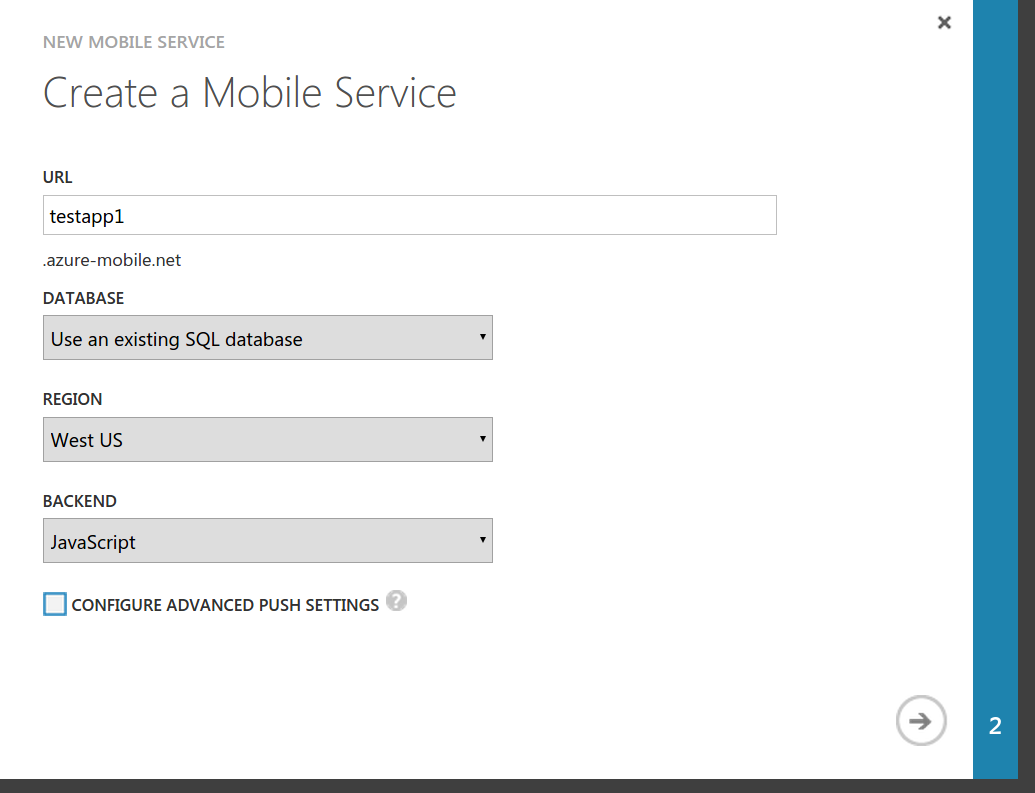
\includegraphics[scale=0.30]{graphics/veliedninger_implementeringAndroid/01-CreateMobileServices.png}}
    \caption{Creating a Mobile Service in Azure}
    %\label{fig:MobileServices}
\end{figure}

\\
\item Opprett navnet du vil at appen skal ha i AzureAD (URL), gjør gjerne dette så beskrivende som mulig.
\\
\item Velg type database du ønsker, her kan du bruke eksisterende SQL database, opprette ny SQL database eller opprette en gratis 20MB SQL database. Databasen må ligge i Azure eller være knyttet til Azure allerede om du skal bruke en eksisterende database.
\\
\begin{itemize}
\item “Region” sier hvor mobile servicen skal lagres, microsoft anbefaler å ha mobile service og database lagret i samme “region”.
\item “Backend” er for å legge inn backend API i tillegg til de spørringene en bruker allerede kan gjøre mot databasen.
\item Sett parametere for databasen. Skriv gjerne ned dette på et sikkert sted, kan hende det tar tid før man får bruk for denne informasjonen igjen. Gjentar at Microsoft anbefaler at databasen ligger i samme region som mobile-service, men dette er ikke et krav.
\end{itemize}
\bigskip

\item Etter at du har opprettet appen går du til Mobile Services i Azure portalen. Velg “Android”, deretter klikk på “create a new android app”
\\
\item Om du allerede har Android studio hoppe over dette punktet. Har du den ikke så last ned og installer android studio.
\\
\item Klikk på create table. Denne oppretter det du trenger for og kjøre eksempelappen. Last ned eksempelappen, det er denne appen denne tutorialen har tatt utgangspunkt i.
\\
\item Åpne appen i android studio, og la android studio kjøre bakgrunnsprosesser ferdig før du gjør noe. Du ser dette på nederste statuslinje i programmet. 
Om Android studio ikke vil godta sertifikatet som følger med prosjektet du har lastet ned så er dette kun knyttet til en https: kobling for og laste ned siste versjon av gradle. Denne pakken kan du hente over http kobling også, om du ønsker en rask løsning på dette.
\\
\begin{itemize}
\item Sertifikatfeilen lå i nedlastningen av siste gradle versjon. Rett opp dette ved å gå inn i filen gradle-wrapper.properties og endre distributionUrl fra https://... til http:// . Filen ligger i prosjektet under /gradle/wrapper/
\item Om Android studio kjører som det skal og ikke gir feilmeldinger kan du kjøre appen nå uten autentisering. Pakken du har lastet ned har automatisk lagt inn knytning til mobile service med uri og key. 
\item Om android sier du må laste ned noen sdk-er, følg bare anbefalte forslag fra android studio. 
\end{itemize}
\bigskip
\begin{figure}[H]
    \centering
    \setlength{\fboxsep}{0pt}%
    \setlength{\fboxrule}{1pt}%
    \fbox{
\includegraphics[scale=0.30]{graphics/veliedninger_implementeringAndroid/01-URLchange.png}}
    \caption{Skjermdump fra gradle-wrapper.properties}
    %\label{fig:MobileServices}
\end{figure}

\\
\item Appen skal nå virke, selv om den er svært enkel. 
\\
\item Sjekk gjerne at du finner igjen oppgavene du lagrer i todolisten i databasetabellen i Azure. Appen og databasen er ikke brukerstyrt, så om du installerer appen på flere telefoner, vi alle telefonene få opp det samme.
\end{enumerate}

\subsection{Del 2 - Legg inn autentisering i applikasjonen.}
\label{subsec:veiledninger_androidBrukerveliedning_del2-LeggInnAutentiseringIApplikasjonen}
For og kunne bruke azure ad som identity provider i appen må dette registrerers både i app koden, i Azure Mobile Service i Azure og i Azure Active Directory. Denne toturialen forutsetter at du har registrert en app i Azure Mobile Service, slik som i del 1 av denne toturialen.
\\
\begin{enumerate}
\item Gå inn i Mobile Services og velg appen du ønsker å legge til identity provder for. 
\\
\item Velg identity og scroll ned listent til den identity provideren du ønsker å bruke. Kopier her url fra appen. 
\\
\begin{figure}[H]
    \centering
    \setlength{\fboxsep}{0pt}%
    \setlength{\fboxrule}{1pt}%
    \fbox{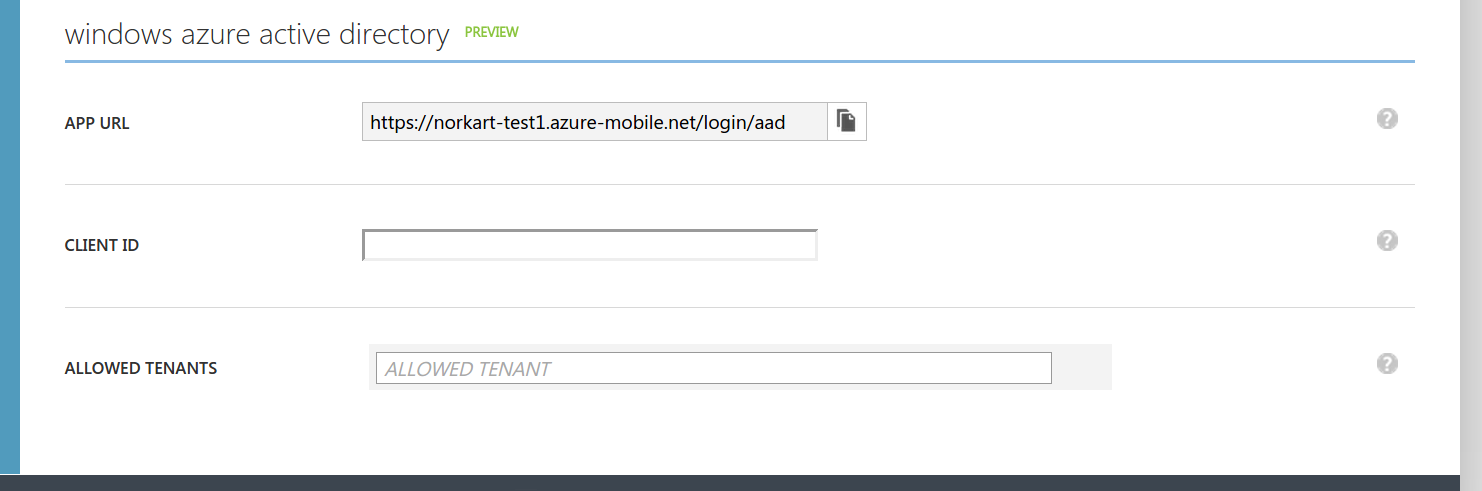
\includegraphics[scale=0.30]{graphics/veliedninger_implementeringAndroid/02-MobileServicesIdentity.png}}
    \caption{Kopier APP URL'en}
    %\label{fig:MobileServices}
\end{figure}
\\
\item Gå inn i den Azure Active Directory du ønsker skal ha tilgang og velg applications.
\\
\begin{itemize}
\item Klikk “ADD” nederst for og legge til en ny applikasjon.
\item Velg “Add an application my organization is developing”
\item Angi navnet applikasjonen skal ha i din Azure Active Directory
\item Velg “WEB APPLICATION AND/OR WEB API”
\item Klikk neste og angi den kopierte APP URL’n i begge boksene. 
\end{itemize}
\bigskip



\item Nå er applikasjonen lagt til i din Azure Active Directory, du skal nå hente ut “Client ID” for applikasjonen, for og knytte applikasjonen i Azure Active Directory sammen med Azure Mobile Services. 
\\
\begin{itemize}
\item Klikk på configure og scroll ned til “CLIENT ID”, kopier denne.
\item Gå tilbake til Azure Mobile Services, finn appen du kopierte URL’en fra tidligere, velg identity og scroll ned windows azure active directory, lim inn “CLIENT ID” i boksen under APP URL. 
\end{itemize}
\bigskip
\begin{figure}[H]
    \centering
    \setlength{\fboxsep}{0pt}%
    \setlength{\fboxrule}{1pt}%
    \fbox{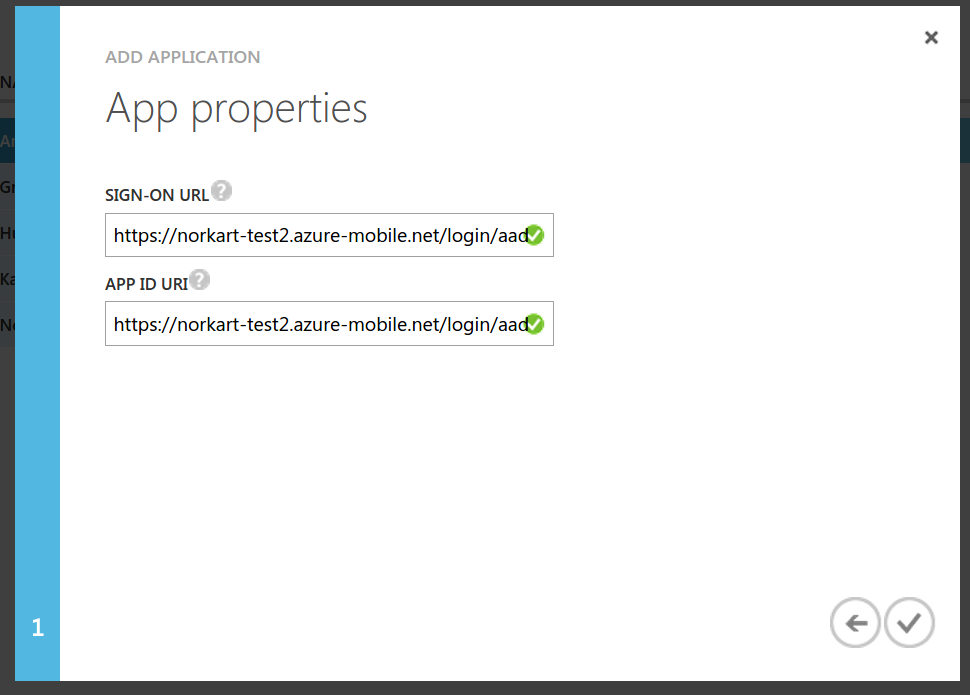
\includegraphics[scale=0.30]{graphics/veliedninger_implementeringAndroid/02-App-properties.png}}
    \caption{Fyll inn URL i begge feltene}
    %\label{fig:MobileServices}
\end{figure}
\\
\item For at du skal kunne logge inn med domenet angitt i din Azure Active Directory må du hente ut dette domenet fra Azure Active Directory og lime det inn i Azure Mobile Services. 
\\
\begin{itemize}
\item Gå til din Azure Active Directory, klikk på “DOMAINS”. 
\item Om du ikke har opprette egne domener vil det være angitt et standard domene. Kopier de domenene du ønsker skal ha tilgang til appen. (kan fortsatt ikke logge inn uten godkjent bruker).
\item Gå til Azure Mobile Services, velg applikasjonen, velg Identity, scroll ned til Windows Azure Active Directory og lim inn domenene i “ALLOWED TENANTS”
\end{itemize}
\bigskip
\begin{figure}[H]
    \centering
    \setlength{\fboxsep}{0pt}%
    \setlength{\fboxrule}{1pt}%
    \fbox{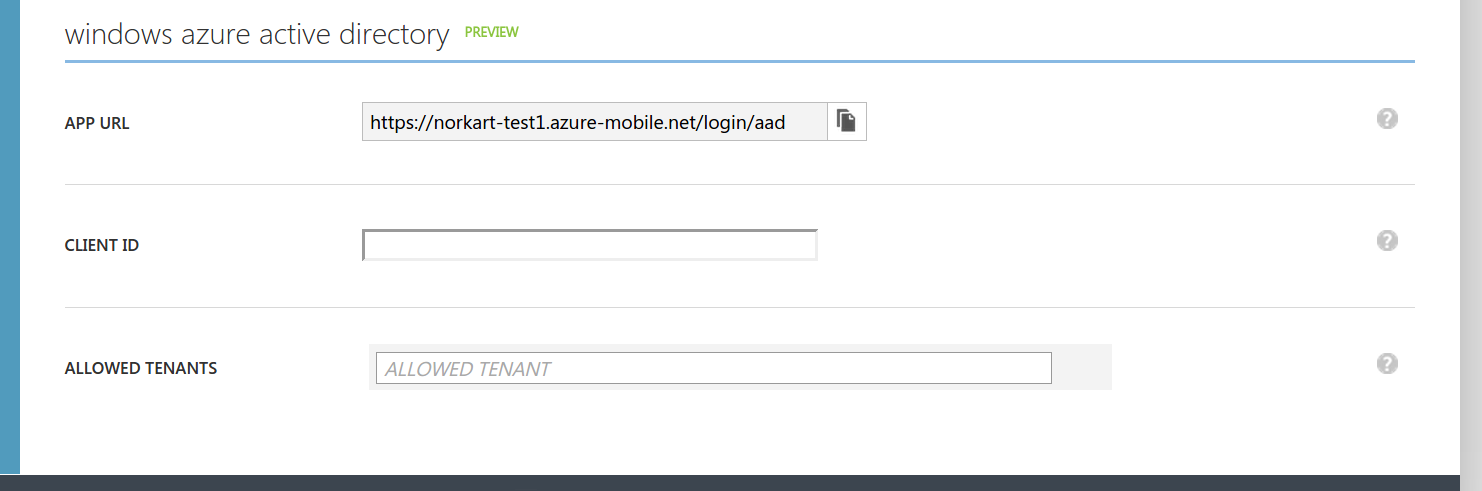
\includegraphics[scale=0.30]{graphics/veliedninger_implementeringAndroid/02-MobileServicesIdentity.png}}
    \caption{Fyll inn app ID og domener}
    %\label{fig:MobileServices}
\end{figure}

\\
\item Vi skal nå hindre andre brukere enn de som er autentiserte og endre data i databasen. 
\begin{itemize}
\item Gi i Azure Mobile Services, velg applikasjonen du skal endre, velg “DATA” derretter “PREMISSIONS” 
\item Endre alle rettighetene til “Only Authenticated Users”
\item Husk å klikke “SAVE” nederst etter at du har endret.
\end{itemize}
\bigskip
\begin{figure}[H]
    \centering
    \setlength{\fboxsep}{0pt}%
    \setlength{\fboxrule}{1pt}%
    \fbox{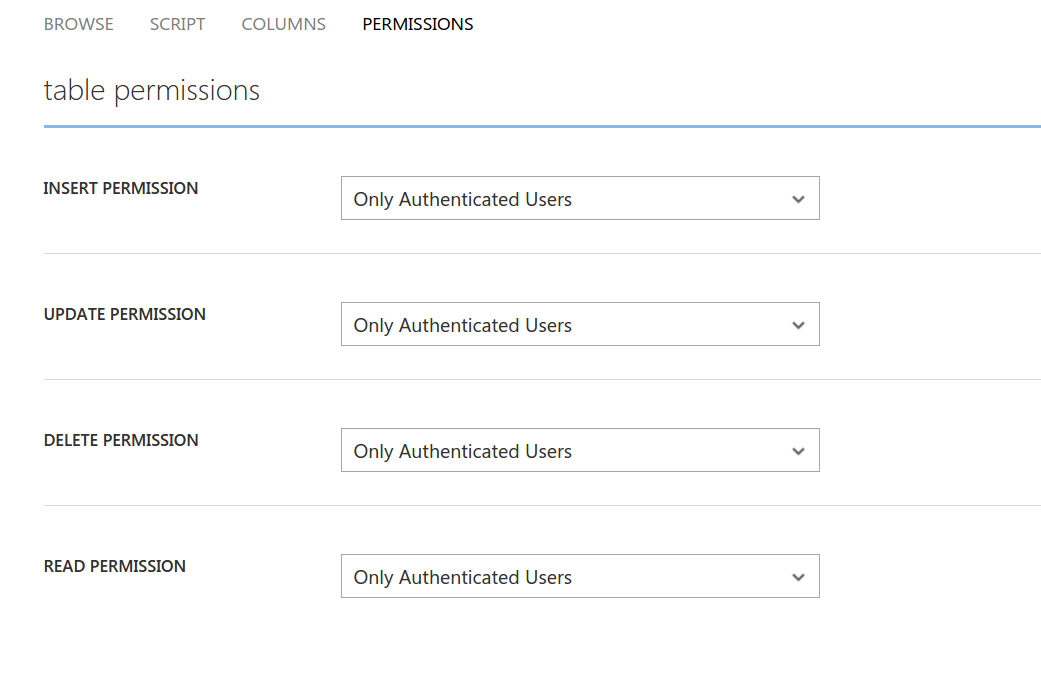
\includegraphics[scale=0.30]{graphics/veliedninger_implementeringAndroid/02-App-premissions.png}}
    \caption{Endre alle "table premissions"}
    %\label{fig:MobileServices}
\end{figure}

\\
\item Vi skal nå legge autentisering inn i app koden i Android studio. Endringene vi gjør her refererer til filnavnet i eksempelprosjektet. Om du ikke bruker eksempelprosjektet legg dette inn i klassen hvor “public void onCreate()” ligger. 
Legg til følgende biblioteker for import.
\\
\begin{lstlisting}[numbers=left, captionpos=b,   caption={Eksempel som viser hvilke biblioteker som bør importeres.}, ]
    
import java.util.concurrent.ExecutionException;
import java.util.concurrent.atomic.AtomicBoolean;

import android.content.Context;
import android.content.SharedPreferences;
import android.content.SharedPreferences.Editor;

import com.microsoft.windowsazure.mobileservices.authentication.MobileServiceAuthenticationProvider;
import com.microsoft.windowsazure.mobileservices.authentication.MobileServiceUser;
\end{lstlisting}
\\
\item Derretter legg til “authenticate()” klassen i samme filen. Kopier inn eksempelkoden nedenfor. Legg merke til at denne koden kan avvike fra veiledninger på nettet, ettersom det her er spesifisert WindowsAzureActiveDirectory som identity provider. 
\\
\begin{lstlisting}[numbers=left, captionpos=b,   caption={Eksempel som viser hvordan authenticate klassen kan se ut.}, ]

private void authenticate() {
    // Login using the Azure AD provider

    ListenableFuture<MobileServiceUser> mLogin = 
    mClient.login(
        mobileServiceAuthenticationProvider.WindowsAzureActiveDirectory);
    
    Futures.addCallback(mLogin, 
        new FutureCallback<MobileServiceUser>() {
        
        @Override
        public void onFailure(Throwable exc) {         
            createAndShowDialog((Exception) exc, "Error");
        }           
        
        @Override
        public void onSuccess(MobileServiceUser user) {
            createAndShowDialog(String.format(
                "You are now logged in - %1$2s",
                user.getUserId()), "Success");
            createTable();  
        }
    });     
}

\end{lstlisting}
\\
\item Derretter skal vi legge til authenticate() klassen. Om du bruker et annet prosjekt enn eksempelprosjektet vil det trolig og legge dette inn etter at du har initert alle objekter men ikke begynt og kjøre noe logikk operasjoner. For demoprosjektet legger vi det inn rett etter at vi har initiert MobileServiceClient i onCreate(); klassen, derretter flytter vi de kodelinjene som lå under MobileServiceClient initieringen ned i en egen klasse som vi kaller createTable(); 
\\
\begin{lstlisting}[numbers=left, captionpos=b,   caption={Eksempel som viser hvordan onCreate() klassen ser ut etter at kode er flytte til en egen createTable() klasse.}, ]

try {
   // Create the Mobile Service Client instance, using the provided
   
   // Mobile Service URL and key
   mClient = new MobileServiceClient(
        "https://norkart-test1.azure-mobile.net/",
        "nSxoADeTLiHClFQShuomNyfOeSGAQL23",
        this).withFilter(new ProgressFilter());
   
   authenticate();
   
   } catch (MalformedURLException e) {
        createAndShowDialog(new Exception("There was an error creating 
        the Mobile Service. Verify the URL"), "Error");
}
\end{lstlisting}
\\
\begin{lstlisting}[numbers=left, captionpos=b,   caption={Eksempel som viser hvordan createTable() klassen kan se ut.}, ]

private void createTable() {

    // Get the Mobile Service Table instance to use
    mToDoTable = mClient.getTable(ToDoItem.class);

    mTextNewToDo = (EditText) findViewById(R.id.textNewToDo);

    // Create an adapter to bind the items with the view
    mAdapter = new ToDoItemAdapter(this, R.layout.row_list_to_do);
    ListView listViewToDo = (ListView) findViewById(R.id.listViewToDo);
    listViewToDo.setAdapter(mAdapter);

    // Load the items from the Mobile Service
    refreshItemsFromTable();
}
\end{lstlisting}
\\
\item Nå skal du kunne kjøre appen og måtte oppgi identity provider for og få logget inn. \\
\item Det er fortsatt mulig å lure seg unna autentiseringen, da vil applikasjonen krasje når den ikke får svaret den forventer fra databasen. Du kan enten legge inn en egen sjekk som sjekker om du er autentisert eller ikke. Alaternativt kan du be applikasjonen avslutte seg selv om brukeren skulle forsøke å omgå autentiseringen. Dette kan du gjøre ved å legge til en finish(); i callBack exception i authenticate() klassen slik som angitt nedenfor.
\\
\begin{lstlisting}[numbers=left, captionpos=b,   caption={Eksempel som viser hvordan onFailure() kan se ut om det legges til en finish(); .},]

Futures.addCallback(mLogin, new FutureCallback<MobileServiceUser>() {
  @Override
  public void onFailure(Throwable exc) {
      createAndShowDialog((Exception) exc, "Error");
      finish();
  }

  @Override
  public void onSuccess(MobileServiceUser user) {
      createAndShowDialog(String.format(
          "You are now logged in - %1$2s",
          user.getUserId()), "Success");
      createTable();
  }
});

\end{lstlisting}
\\
\item Nå skal du kunne logge inn i applikasjonen. Det er ikke enda lagt til noen logg-ut knapp. For å teste at du kan logge inn med ulike brukere må du fjerne appdata i innstillinger for applikasjonen i android systemet. 
\end{enumerate}


\chapter{Gammel Kravspesifikasjon}
\label{chap:kravspesifikasjonGammel}
Kravspesifikasjonen gjelder for SSO løsningen prosjektet skal prosjektere. Ved behov gjelder også kravspesifikasjonen for eventuelle prototyper som lages for og bevise eller utdype ulike tekniske valg og løsninger.

\section{Hvordan kravspesifikasjon er utarbeidet}
\label{sec:kravspesifikasjonGammel_hvordanKravspesifikajsonErUtarbeidet}
Prosjektgruppen brukte et par uker på å sette seg inn i ulike autentiseringsløsninger før kravspesifikasjonen ble utarbeidet. Ingen på prosjektgruppen regnet seg selv om dyktige på fagområdet autentisering og autorisering av brukere, vi ga oss selv derfor en kort periode med faglig dypdykk før vi gikk i gang med utarbeidelse av en kravspesifikasjon for SSO løsningen Norkart ønsket.
\bigskip
Kravspesifikasjonen ble utarbeidet av prosjektgruppen på forespørsel fra product owner hos Norkart. Prosjektgruppen har jevnlig dialog med product owner for og sikre at oppgaven og kravspesifikasjon henger sammen.
\bigskip
I forhold til målbare data oppgitt i seksjon \ref{sec:kravspesifikajsonGammel_operasjonelleKrav} -  \nameref{sec:kravspesifikajson_operasjonelleKrav} på side \pageref{sec:kravspesifikajson_operasjonelleKrav} tok vi utgangspunkt i hva Norkart så for seg som et ekstremsenario for løsningen om de skulle selge svært mye og ha svært mye aktivitet. 

\section{Funksjonelle krav til løsningen}
\label{sec:kravspesifikajsonGammel_funksjonelleKrav}
Funksjonelle krav brukes for å si hva systemet skal utføre, og hvordan systemet skal reagere på ulike situasjoner. 

\subsection{Overordnet use case diagram}
\label{subsec:kravspesifikajsonGammel_funksjonelleKrav_overordnetUseCase}
For å beskrive hva endelig løsning skal inneholde av funksjonalitet og roller er det laget et overordnet Use Case (se figur \ref{fig:OverordnetUseCase-a} på side \pageref{fig:OverordnetUseCase}). Dette use caset er en skisse av Norkart ID som endelig løsning. For å begrense oppgaven ser vi for oss å fokusere på egenadministrasjon og innloggingsmekanismer. Dersom det blir tid til mer blir vi enig om hva som skal gjøres i samråd med Norkart. Nedenfor vil du kunne lese en kort forklaring av roller og funksjoner.

\begin{figure}[h]
    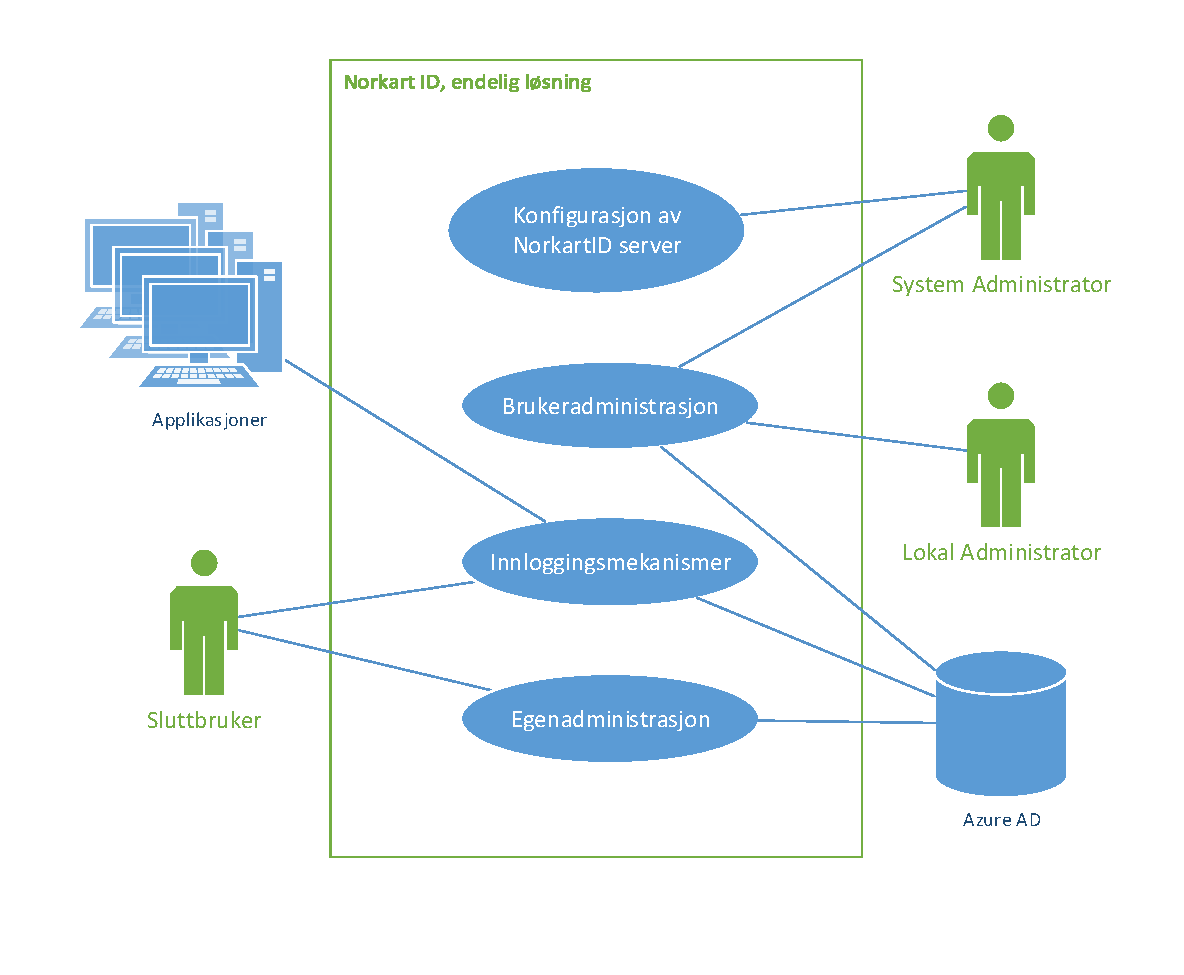
\includegraphics[scale=0.65]{graphics/OverordnetUseCase-a}
    \caption{Overordnet Use Case for endelig løsning av Norkart ID}
    \label{fig:OverordnetUseCase-a}
\end{figure}

\subsubsection*{System Administrator}
System administrator er rollen som setter opp hvordan Norkart ID systemet skal kobles sammen med applikasjonsserverene. System administrator har også mulighet til å administrere alle brukere som er tilkoblet systemet. 

\subsubsection*{Lokal Administrator}
Denne rollen har til hensikt å gjøre passordgjennoppretting og administrasjon av brukeretilgang tilgjengelig for bedriften som benytter seg av programvaren. Dette resulterer i redusert press på Norkart kundeservice. 

\subsubsection*{Azure AD}
Azure AD er brukerdatabasen Norkart ID skal benytte for å lagre brukerdata og tilgangsstyring. Den skal også kunne vedlikeholdes uten å gå via Norkart ID om dette er ønskelig. Ettersom all brukerdata lagres i Azure AD må alle roller som har mulighet til å endre brukerdata også kunne skrive eller oppdatere data igjennom Norkart ID. Azure AD brukes for å hente ut oppslag for hver eneste forespørsel om autentisering og autorisasjon av brukere mot applikasjoner.

\subsubsection* {Applikasjoner}
Applikasjoner er i dette tilfellet de applikasjonene Norkart ID skal autorisere brukere for å bruke. Norkart ID må kjenne til hvor og hvordan brukerne som autoriseres skal kontakte applikasjonene de er autoriserte for å bruke. Etter at en bruker logger seg inn med Norkart ID vil brukeren få informasjonsom trengs for å knytte seg til applikasjonene.

\subsubsection* {Sluttbruker}
Sluttbruker bruker Norkart ID som autentisering og autoriseringstjeneste. Dette er brukeren som logger inn med Norkart ID og får tilgang til tjenestene Norkart tilbyr.

\subsection {Use case diagram for prototype}
\label{subsec:prototype_use_case}
For å få et dypere innblikk av hva selve prototypen skal inneholde er det laget et use case diagram, se figur \ref{fig:PrototypeUseCase}, som inneholder roller og funskjoner basert på innloggingsmekanismer og egenadministrasjon i overordnet use case, se figur \ref{fig:OverordnetUseCase}. Innlogggingsmekanismer er her delt opp i tre funksjoner og e-post er tatt med som eksternt system. 

\begin{figure}[h]
    \includegraphics[scale=0.65]{graphics/PrototypeUseCase}
    \caption{Use Case Diagram for prototypen av Norkart ID }
    \label{fig:PrototypeUseCase}
\end{figure}

\subsubsection* {Applikasjoner}
For at bruker skal kunne logges inn må Norkart ID vite hvilken applikasjon bruker vil logge inn på. Derfor trenger rollen applikasjoner, se figur  \ref{fig:PrototypeUseCase}, kun tilgang til logg inn funksjonalitet.

\subsubsection* {Sluttbruker}
Sluttbruker kan benytte all funksjonalitet i prototypen.

\subsubsection*{Azure AD}
Ettersom bruker må autentiseres for å logge inn og ut og bruke glemt passord funksjonalitet  må Norkart ID ha tilgang til Azure AD for å utføre disse funskjonene. Norkart ID må også ha tilgang til Azure Ad for å endre brukerdata under egenadministrasjon.

\subsubsection* {E-post}
For at Norkart ID skal kunne gjennomføre glemt passord funksjonalitet trenger den tilgang til en E-post server. Hvis en bruker har glemt passord skal Norkart ID sende en resett passord link på e-post til brukeren.

\subsection{Høynivå use case beskrivelser}
\label{subsec:kravspesifikasjonGammel_funksjonelleKrav_hoyNivaa}
4 høynivå use case beskrivelser er definert for å beskrive funksjonalitet i løsningen.

\begin{framed}
    \begin{tabular}{l p{9cm}}
        \textbf{Use case:} & Logg inn \\
        \textbf{Aktører:} & Sluttbruker, Applikasjon og Azure AD \\
        \textbf{Mål:} & Bruker skal kunne få tilgang til ønsket applikasjon. Applikasjon skal være sikker på at bruker har tilgang \\
        \textbf{Beskrivelse:} & Når bruker skriver inn brukernavn og passord skal brukeren autentiseres og få tilgang til applikasjonen den ønsker å jobbe på.
    \end{tabular}
\end{framed}
\begin{framed}
    \begin{tabular}{l p{9cm}}
        \textbf{Use case:} & Logg ut \\
        \textbf{Aktører:} & Sluttbruker og Azure AD \\
        \textbf{Mål:} & Bruker skal kunne få logget ut av ønsket applikasjon og fra alle andre tjenester \\
        \textbf{Beskrivelse:} &  Når bruker klikker logg ut skal brukeren bli utlogget i alle systemet, både web, mobil og applikasjonsnivå. En singel-sign-out(for aktivt token) måte hvor man slipper å måtte logge ut individuelt i alle systemer.
    \end{tabular}
\end{framed}
\begin{framed}
    \begin{tabular}{l p{9cm}}
        \textbf{Use case:} & Glemt passord \\
        \textbf{Aktører:} & Sluttbruker, Azure AD og E-post \\
        \textbf{Mål:} & Bruker skal kunne få mulighet sette nytt passord og få logget inn igjen. \\
        \textbf{Beskrivelse:} &  Bruker skal kunne hente ut passord selv til sin brukerprofil uten å måtte kontakte kundeservice. Her er tanken at man skal kunne motta en epost med en reset link hvor du kommer inn direkte til hvor du skal opprette nytt passord.
    \end{tabular}
\end{framed}
\begin{framed}
    \begin{tabular}{l p{9cm}}
        \textbf{Use case:} & Egenadministrasjon \\
        \textbf{Aktører:} & Sluttbruker og Azure AD \\
        \textbf{Mål:} &  Bruker skal kunne endre på registrerte opplysning inne på sin brukerprofil. \\
        \textbf{Beskrivelse:} &  Når bruker er autentisert skal han kunne gå inn for å endre på sin profil. Det er her sluttbruker får tilgang til epost, telefon, generelle opplysning som er registrert. Brukeren har her mulighet til å endre de attributtene som går an og endre. Dette er en egen nettside hvor bruker får tilgang til etter autentisering.
    \end{tabular}
\end{framed}

\subsection{User Stories}
\label{subsec:kravspesifikasjonGammel_funksjonelleKrav_userStories}
For å få en dypere forståelse av hva slags funksjonalitet som trengs for å overholde kravene til oppgaven har vi utarbeidet user stories som viser hva de forskjellige brukerne av applikasjonen skal kunne å utføre. De er utarbeidet ut fra use case diagram for prototypen, (se figur \ref{fig:PrototypeUseCase} på side \pageref{fig:PrototypeUseCase}), og oppgavens operasjonelle krav (se seksjon \ref{sec:kravspesifikajson_operasjonelleKrav}).


\section{Operasjonelle krav til løsning}
\label{sec:kravspesifikasjonGammel_operasjonelleKrav}
Operasjonelle krav brukes for å beskrive kvaliteten på systemet, dette kan være i form av standarder som benyttes, målinger som skal være innenfor en gitt grense og kostnadder.

\subsection{Ytelse}
\label{subsec:kravspesifikasjonGammel_operasjonelleKrav_ytelse}
\begin{itemize}
\item Løsningen skal som minimum takle 10 000 brukere innlogget samtidig.
\item Løsningen skal håndtere pålogging av 100 brukere i minuttet.
\item Løsningen skal bygges for å være skalerbar.
\item Det skal ta mindre enn et sekund å autentisere en bruker for de systemene brukeren er autorisert for å bruke.
\item Om belastning på NorkartID serversystemet skulle bli så høy at overordnede krav til innloggingstid ikke overholdes vil operasjoner og forespørsler fra brukere behandles etter FIFO-kø prinsippet.
\end{itemize}

\subsection{Implementasjon}
\label{subsec:kravspesifikasjonGammel_operasjonelleKrav_implementasjon}
\begin{itemize}
\item NorkartID skal fungere som en autentiserings- og autoriseringsledd mellom brukerne og tjenestene Norkart tilbyr.
\item Løsningen skal kjøres på en Microsoft Windows server 2012 eller nyere.
\item Løsningen skal benytte Azure AD brukerdatabase.
\item Innloggingsløsningen skal baseres på OpenID Connect biblioteker.
\item NorkartID skal designes for eksterne brukere.
\end{itemize}

\subsection{Standarder}
\label{subsec:kravspesifikasjonGammel_operasjonelleKrav_standarder}
\begin{itemize}
\item Løsningen skal tilfredstille kravene til OpenID Connect standardene.
\item Løsningen skal igjennom bruk av OpenID Connect tilfredstille sikkerhetsmekanismene gitt ved å burke OAuth 2.0
\item All kommentering og dokumentasjon av kildekode skal gjøres i henhold til normer gitt for programeringsspråkene som brukes i prosjektet.
\end{itemize}

\subsection{Pålitelighet}
\label{subsec:kravspesifikasjonGammel_operasjonelleKrav_pålitelighet}
\begin{itemize}
\item Pålitelighet i forhold til oppetid av Azure plattformen medregnes ikke i dette prosjektet. 
\item Azure AD skal håndteres slik at den aldri skal trenge å taes ned. 
\item Systemet skal designes for å ha en oppetid på minimum 99,9 \%, det vil si 10 minutter nedetid for vedlikehold i uken.
\item NorkartID serveren, Open ID Connect og Azure AD skal kunne vedlikeholdes individuelt.
\item Systemet stiller ingen krav til å kunne oppdateres mens det kjører.
\item Kundestøtte for NorkartID vil implementeres hos eksisterende kundeservice.
\end{itemize}

\subsection{Brukervennlighet}
\label{subsec:kravspesifikasjonGammel_operasjonelleKrav_brukervennlighet}
\begin{itemize}
\item Løsningen skal følge regler for universell utforming (se lover og regler)
\item Bruker skal kunne bruke samme påloggingsinformasjon mot alle systemene til Norkart.
\item Brukere skal selv kunne administrere brukerprofil og passord
\item Brukergrensesnittet skal være så intuitivt at det tar mindre enn 2 sekunder å skjønne hvor brukerid felt, passord felt og innloggingsknappen er.
\item Brukergrensesnittet på løsningen skal være skrevet på norsk.
\item Brukergrensesnittets design skal skape gjenkjennelighet til Norkart.
\item Fremdriftsindikator skal brukes der det er hensiktsmessig for å gi brukeren tilbakemelding.
\item Når bruker lager passord skal det gis indikasjon på om passordkravene tilfredstilles.
\end{itemize}

\subsection{Lover og regler}
\label{subsec:kravspesifikasjonGammel_operasjonelleKrav_lover_regler}
\begin{itemize}
\item Systemet skal håndtere data i samsvar med lov for Norsk personvern
\item Systemet skal følge forskrift om universell utforming av informasjons- og kommunikasjonsteknologiske (IKT)-løsninger
\end{itemize}

\subsection{Intraoperabilitet}
\label{subsec:kravspesifikasjonGammel_operasjonelleKrav_intraoperabilitet}
\begin{itemize}
\item Systemets API skal kunne kommunisere over standard http protokoll.
\item Systemets API skal støtte autentisering, glemt passord funksjonalitet og fornying av økt.
\item Brukergrensesnitt på løsningen skal være responsivt.
\item Systemet skal ha støtte for Single Sign On på Microsoft Windows 8 (eller nyere windows systemer).
\end{itemize}

\subsection{Sikkerhet og autentiseringskrav}
\label{subsec:kravspesifikasjonGammel_operasjonelleKrav_sikkerhet}

\begin{itemize}
\item Brukerdata løsningen trenger: Fullt navn, selskap, mail, passord, mobil, sist innlogget og gjeldende autentiserte enheter. 
\item All lagring av brukerdata skal beskyttes i forhold til trusselbilde. 
\item Ingen passord skal sendes eller lagres i klartekst.
\item Systemet skal følge generelle normer innenfor autentisering
\item Minimumskrav for passordlengde er 8 tegn.
\item Minimumskrav for passordkompleksitet er minimum en stor og en liten bokstav, og minimum et tall. 
\item Etter 5 feilede innloggingsforsøk mot en bruker id skal det legges inn ventetid på 1 minutt før det tillattes nytt innloggingsforsøk mot samme bruker id.
\item Ved feil passord eller brukernavn skal det kun stå at innlogging feilet. 
\item Ved glemt passord skal det sendes link til bruker for generering av nytt passord. Denne linken skal kun være gyldig i 20 minutter.
\item En sesjon er kun gyldig 6 timer før den må fornyes.
\item En bruker som logger inn via en nettleser  autentiseres for alle web applikasjoner brukeren har tilgang til i den nettleseren.
\item En bruker som logger inn i en mobil applikasjon autentiserers kun til denne applikasjonen
\item En bruker som logger inn i en desktop applikasjon autentiseres kun til denne applikasjonen.
\end{itemize}

\subsection{Klientkrav}
\label{subsec:kravspesifikasjonGammel_operasjonelleKrav_klientkrav}
\begin{itemize}
\item Det kreves at klienten har tilgang på en nettleser som leser HTML5, CSS3 og JavaScript.
\item Klienten må gi tilgang til cookies for å bruke Single Sign On funksjonaliteten i nettleser.
\item Klienten må ha skriverettigheter i maskinens register for å bruke Single Sign On funksjonaliteten på skrivebordsapplikasjoner.
\item Det kreves at klienten er tilkoblet internett eller i nettverk med NorkartID serveren.
\item Det kreves at klienten har nettverkshastighet tilsvarende 0,4 Mbit eller høyere for garantert stabil tilkobling til tjenesten (stabil Edge eller høyere tilkobling).
\end{itemize}


\section{Krav til resultat av prosjektoppgaven}
\label{sec:kravspesifikasjonGammel_kravTilResultatAvProsjektoppgaven}
{\color{red}TODO}\\
Oppgaven skal skrives etter regningslinjer gitt for bachelor og masteroppgaver ved Høyskolen i Gjøvik.
\\
\\
\href{http://www.hig.no/content/download/30554/364363/file/Retningslinjer%20for%20mastergradsoppgaver%20og%20st%C3%B8rre%20studentoppgaver%20p%C3%A5%20bachelorniv%C3%A5%20ved%20H%C3%B8gskolen%20i%20Gj%C3%B8vik_des2010_v1201.pdf}{Link til retingslinjene}


\chapter{IdentityServer3}
\label{chap:IdentityServer3}
Prosjektgruppen begynte prosjektet med å se på mulig implementasjon av en løsning basset på rammeverket IdentityServer3. Dette vedlegge beskriver hvordan en implementasjon av autentiseringssystemet kunne sett ut om vi hadde bassert systemet på IdentityServer3.

\section*{Arkitekturvalg}
\label{sec:identityServer3_arkitekturvalg}
For å få et arkitekturisk overblikk over systemet brukes SAD fra RUP med Philippe Kruchten’s 4+1 view modell (se figur \ref{fig:4+1illustrasjonssikkse}). 4+1 tar utgangspunkt i at det overordnede use case diagrammet (se figur \ref{fig:OverordnetUseCase}) er definert. Det overordnede use case diagrammet regnes som '+1' av de '4+1' og befinner seg i midten av modellen (figur \ref{fig:OverordnetUseCase}). De fire views'ene som som ligger rundt senarioene i Use Caset har til hensikt å illustrere ulike synsvinkler inn mot senarioene (senarione er beskrevet i kapittel \ref{subsec:use_case_logge_inn}). Setter man alle delene av 4+1 modellen sammen kan man være relativt sikker på at de aller fleste av problemstillingene ved systemet i forhold til arkitektur blir dekt. 

\begin{figure}[H]
    \centering
    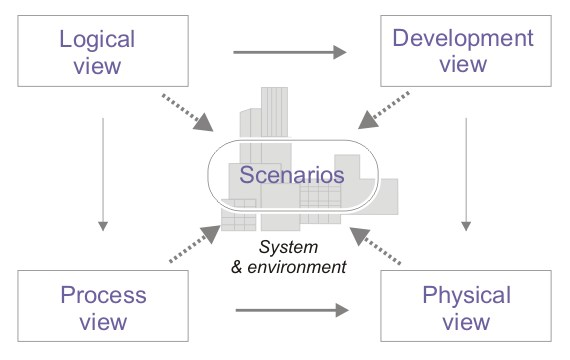
\includegraphics[scale=0.50]{graphics/04-arkitektur/4+1_Architectural_View_Model.jpg}
    \caption{4+1 illustrasjonsskisse. Hentet fra wikipedia}
    \label{fig:4+1illustrasjonssikkse}
\end{figure}

\section{Use case View}
\label{sec:use_case_view}
Vi har laget 4 extended use caser: logge inn, logge ut, glemt passord og egenadministrasjon. Ved å gjøre dette fikk vi større innblikk i det vi ser på som den viktigste funksjonaliteten.

\subsection{Logge inn}
\label{subsec:use_case_logge_inn}
\newline \textbf{Use case:} Logge inn på en webtjeneste
\newline \textbf{Aktør:}	Sluttbruker, Applikasjon og Azure AD
\newline \textbf{Mål:} Bruker skal kunne få tilgang til ønsket applikasjon. Applikasjon skal være sikker på at bruker har tilgang.
\newline \textbf{Beskrivelse:} Når bruker skriver inn brukernavn og passord skal brukeren autentiseres og få tilgang til applikasjonen den ønsker å jobbe på.
\newline \textbf{Pre-betingelser:} Bruker finnes allerede i systemet. 
\newline \textbf{Post betingelser:} Autentisert i alle webtjenester via Norkart ID.
\newline \textbf{Spesielle krav:} Har tilgang til NorkartID i nettverk eller via web.
\newline \textbf{Detaljert hendelsesforløp:}
\newline
\newline \textbf{Brukerhandling}
\newline 1. Use casen begynner når brukeren går til nettsiden for å bruke programmet.
\newline 2. Klient ber bruker om å  logge inn med brukernavn og passord.
\newline 3. Sluttbruker skriver inn innloggingsdetaljer.
\newline 4. Klient sender innloggings request til OpenID Connect
\newline 8. Bruker sender autentiseringskoden til OpenID Connect automatisk tilklienten.
\newline 9. Klient sender inn autentiseringskode for å motta token.
\newline 11. Token valideres i klienten.
\newline
\newline \textbf{Systemrespons}
\newline 5. OpenID Connect autentiserer sluttbruker mot Azure AD.
\newline 6. Azure AD autentiserer sluttbruker.
\newline 7. Norkart ID sender autentiseringskode til sluttbruker.
\newline 10. OpenID Connect sender en ID token og Access token til klienten (RP).
\newline

\begin{figure}[H]
    \centering
    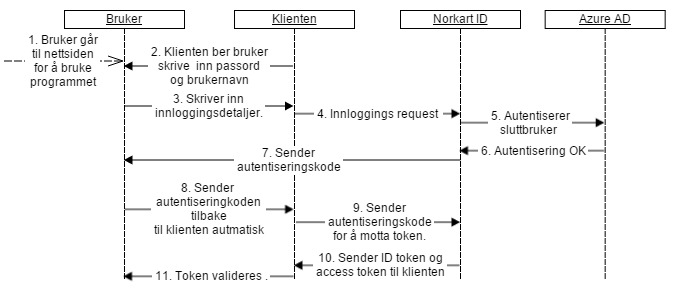
\includegraphics[scale=0.55]{graphics/04-arkitektur/UseCaseSekveknsdiagramLoggeInn.jpg}
    \caption{Sekvensdiagram 'logge inn'}
    \label{fig:skevensdiagramLoggInn}
\end{figure}

\noindent Figur \ref{fig:skevensdiagramLoggInn}, viser sekvensdiagrammet for når en bruker logger inn, og hvordan systemet kommer til å håndtere en slik spørring. Dette er en litt forenklet representasjon av hva som står under detaljert hendelsesforløp.
\newline
\newline
Nedenfor vises det ulike hendelsesforløp der det er bruker feil eller systemfeil.
\newline

\newline \textbf{Brukerfeil}
\begin{itemize}
\item Bruker skriver feil passord
\newline Bruker bes om å skrive brukernavn og passord på nytt og beskjed til bruker vil være: Innlogging feilet.
\item Bruker skriver feil brukernavn
\newline Bruker bes om å skrive inn brukernavn og passord på nytt og beskjed til bruker vil være: Innlogging feilet.
\item Gjentatt forsøk på innlogging med ugyldige opplysninger
\newline Bruker bes etter 5 forsøk om å vente 5 minutter før det prøves igjen. Skulle det igjen ikke gå går det 20 minutter til neste gang bruker kan prøve.
\end{itemize}

\bigskip \textbf{Systemfeil}
\begin{itemize}
\item Lang innloggingstid
\newline Om innloggings skulle ta mer enn 2 sekunder skal det gies beskjed til bruker at det tar unormalt lang tid å logge inn. Skulle det feile så bes bruker om å prøve en gang til. Om det skulle feile enda en gang til bes det om å ta kontakt med support, enten lokalt eller eksternt.
\item Innlogging ikke mulig å gjennomføre
\newline Skulle innlogging feile bes bruker om å prøve på nytt i første omgang. Om dette ikke skulle løse problemet bes bruker om å ta kontakt med support, enten lokalt eller eksternt.
\end{itemize}


\subsection{Logge ut}
\label{subsec:use_case_logge_ut}
\newline \textbf{Use case:} Logge ut via en webtjeneste
\newline \textbf{Aktør:}	Sluttbruker og Azure AD
\newline \textbf{Mål:} Bruker skal kunne få logget ut av ønsket applikasjon og fra alle andre tjenester.
\newline \textbf{Beskrivelse:} Når bruker klikker logg ut skal brukeren bli utlogget i alle systemet, både web, mobil og applikasjonsnivå. En singel-sign-out(for aktivt token) måte hvor man slipper å måtte logge ut individuelt i alle systemer.
\newline \textbf{Pre-betingelser:} Er allerede innlogget.
\newline \textbf{Post betingelser:} Blir logget ut i alle tjenester/sletter token slik at bruker er ute av alle webtjenester
\newline \textbf{Detaljert hendelsesforløp:}
\newline
\newline \textbf{Brukerhandling}
\newline 1. use casen begynner når brukeren går til tjenesten for å logge ut.
\newline 2. Bruker klikker logg ut.
\newline 3. Klient sender request til OpenID Connect.
\newline 5. Token blir slettet og viser i klienten at man har blitt logget ut.
\newline
\newline \textbf{Systemrespons}
\newline 4. OpenID Connect håndterer utloggings request og trigger utloggingskall til alle tjenester
\newline
\newline
Bruker kommuniserer med Norkart ID igjennom en klient som viser hvordan man skal gå frem for å kunne logge inn, se figur \ref{fig:skevensdiagramLoggUt}. Under ser du logge ut sekvensdiagrammet og hvordan det kommer til å bli:
\newline

\begin{figure}[H]
    \centering
    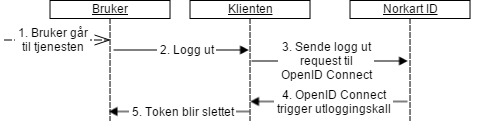
\includegraphics[scale=0.55]{graphics/04-arkitektur/UseCaseSekveknsdiagramLoggeUt.jpg}
    \caption{Sekvensdiagram 'logge ut'}
    \label{fig:skevensdiagramLoggUt}
\end{figure}

\textbf{Brukerfeil}
\begin{itemize}
\item Bruker logger ikke ut før han forlater arbeidsstasjonen
\newline Bruker bli automatisk logget ut etter et tidsintervall på 6 timer slik at om man skulle glemme å logge seg ut må man reautentisere seg når man returnerer.
\end{itemize}

\bigskip \textbf{Systemfeil}
\begin{itemize}
\item Bruker blir ikke logget ut av alle webtjenestene
\newline Bruker får beskjed om at det ikke var mulig å gjennomføre forespørsel og bes om å gå inn direkte på Norkart ID tjeneste og prøve på nytt. Om dette ikke skulle være nok skal det reises et flagg om at det er problem med utlogging.
\end{itemize}


\subsection{Glemt passord}
\label{subsec:use_case_glemt_passord}
\newline \textbf{Use case:} Glemt passord på websiden
\newline \textbf{Aktør:}	Sluttbruker, Azure AD og E-post
\newline \textbf{Mål:} Bruker skal kunne få mulighet sette nytt passord og få logget inn igjen.
\newline \textbf{Beskrivelse:} Bruker skal kunne hente ut passord selv til sin brukerprofil uten å måtte kontakte kundeservice. Her er tanken at man skal kunne motta en epost med en reset link hvor du kommer inn direkte til hvor du skal opprette nytt passord.
\newline \textbf{Pre-betingelser:} Bruker er allerede registrert med epostadresse.
\newline \textbf{Detaljert hendelsesforløp:}
\newline
\newline \textbf{Brukerhandling}
\newline 1. Use casen begynner når brukeren går til nettsiden få nytt passord.
\newline 2. Bruker klikker på glemt passord.
\newline 3. Bruker skriver inn epostadressen sin og bekrefter en captcha test.
\newline 7. Bruker blir bedt om å henvende seg til epost innboksen sin for å forsette.
\newline
\newline \textbf{Systemrespons}
\newline 5. Systemet slår opp bruker i databasen.
\newline 6. Det genereres en resetlink og den blir sendt til registrert epost.
\newline
\newline
Siden vi lager en singel-sign-in er det vel så viktig med en single-sign-out hvor du blir logget ut i alle tjenestene. Dette gjøres med tanke på sikkerhet og for å gjøre det lettere for bruker å kunne logge ut av systemet.
\newline
\newline
Nedenfor vises det ulike hendelsesforløp der det er bruker feil eller systemfeil.
\newline

\begin{figure}[H]
    \centering
    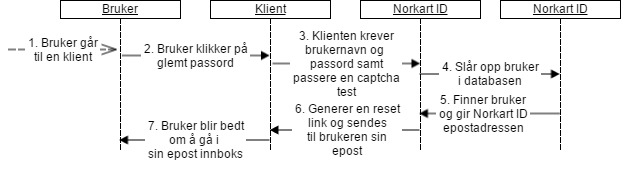
\includegraphics[scale=0.55]{graphics/04-arkitektur/UseCaseSekveknsdiagramGlemtPassord.jpg}
    \caption{Sekvensdiagram 'glemt passord'}
    \label{fig:skevensdiagramGlemtPassord}
\end{figure}

\noindent \textbf{Brukerfeil}
\begin{itemize}
\item Bruker oppgir ugyldig format på epost adresse
\newline Det gies en beskjed til bruker om at det er brukt feil format på epostadressen som er skrevet inn og presenterer a@b.c som format.
\item Bruker feiler på capcha sjekken
\newline Refresher siden 
\end{itemize}

\bigskip \textbf{Systemfeil}
\begin{itemize}
\item Epost blir ikke sendt ut.
\newline Det gjøres ingen sjekk av systemet annet enn at linken som blir sendt ut er gyldig i 30 minutter. Hvis den ikke kommer fram til bruker får bruker selv prøve på nytt.
\end{itemize}

\subsection{Egenadministrasjon}
\label{subsec:use_case_egenadministrasjon}
\newline \textbf{Use case:} Egenadministrasjon av brukerprofil
\newline \textbf{Aktør:}	Sluttbruker og Azure AD
\newline \textbf{Mål:} Bruker skal kunne endre på registrerte opplysning inne på sin brukerprofil.
\newline \textbf{Beskrivelse:} Når bruker er autentisert skal han kunne gå inn for å endre på sin profil. Det er her sluttbruker får tilgang til epost, telefon, generelle opplysning som er registrert. Brukeren har her mulighet til å endre de attributtene som går an og endre. Dette er en egen nettside hvor bruker får tilgang til etter autentisering.
\newline \textbf{Pre-betingelser:} Er allerede innlogget i systemet
\newline \textbf{Post betingelser:} Endringer skjer i sanntid og bruker og brukerprofil tar i bruk endringer i sanntid.
\newline \textbf{Detaljert hendelsesforløp:}
\newline
\newline \textbf{Brukerhandling}
\newline 1. Use casen begynner når brukeren går til nettsiden for å endre brukerdata.
\newline 2. Viser siden for egenadministrasjon.
\newline 4. Ved lagring kan bruker forsatt gjøre endringer eller logge ut.
\newline
\newline \textbf{Systemrespons}
\newline 3. Endringer gjort fra klient blir overført til database og klient.
\newline

\begin{figure}[H]
    \centering
    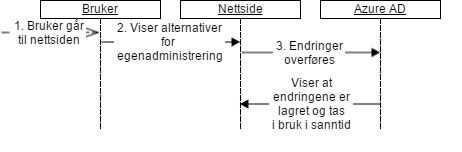
\includegraphics[scale=0.55]{graphics/04-arkitektur/UseCaseSekveknsdiagramEgenadministrasjon.jpg}
    \caption{Sekvensdiagram 'egenadministrasjon'}
    \label{fig:skevensdiagramEgenadministrasjon}
\end{figure}

\noindent Denne sees på som viktig for å kunne muliggjør noen form for selvadministrering til brukerne som igjen resulterer til mindre trykk på Norkart kundeservice.
\newline
\newline Nedenfor vises det ulike hendelsesforløp der det er bruker feil eller systemfeil.
\newline
\newline \textbf{Brukerfeil}
\begin{itemize}
\item Ikke innlogget
\newline Bruker skal bli henvist til innloggingssiden når bruker ikke har valid token eller ikke er innlogget.
\item Endrer til ugyldig informasjon i brukerprofilen
\newline Når bruker endrer opplysninger skal disse sjekkes ved hjelp av enten Javascript sjekker eller biblioteker for å klient sjekke at informasjonen riktig skrevet før den går inn i systemet. 
\end{itemize}

\bigskip \textbf{Systemfeil}
\begin{itemize}
\item Om systemet ikke klarer å behandle endringsforespørsel
\newline Systemet skal gi beskjed tilbake om endringer er OK eller ikke. Ved tilfeller der det ikke er OK bes bruker å prøve på nytt og hvis feilen vedvarer om å ta kontakt med Norkart.
\end{itemize}

\section{Logisk View}
\label{sec:logisk_view}
I forhold til 4+1 modellen har det logiske viewet til hensikt å illustrere sluttbrukers perspektiv på produktet. For å øke skalerbarheten og sikkerheten til systemet er det brukt en trelags arkitektur hvor Model View Controller (MVC) er brukt som arkitekturpattern i det øverste laget. MVC er brukt for å skape mindre avhengigheter i systemet og for å redusere kodekompleksiteten. For å få en oversikt over lag og klasser er det utviklet et design klassediagram, se figur \ref{fig:LogiskViewKlassediagram}.

\begin{figure}[H]
    \centering
    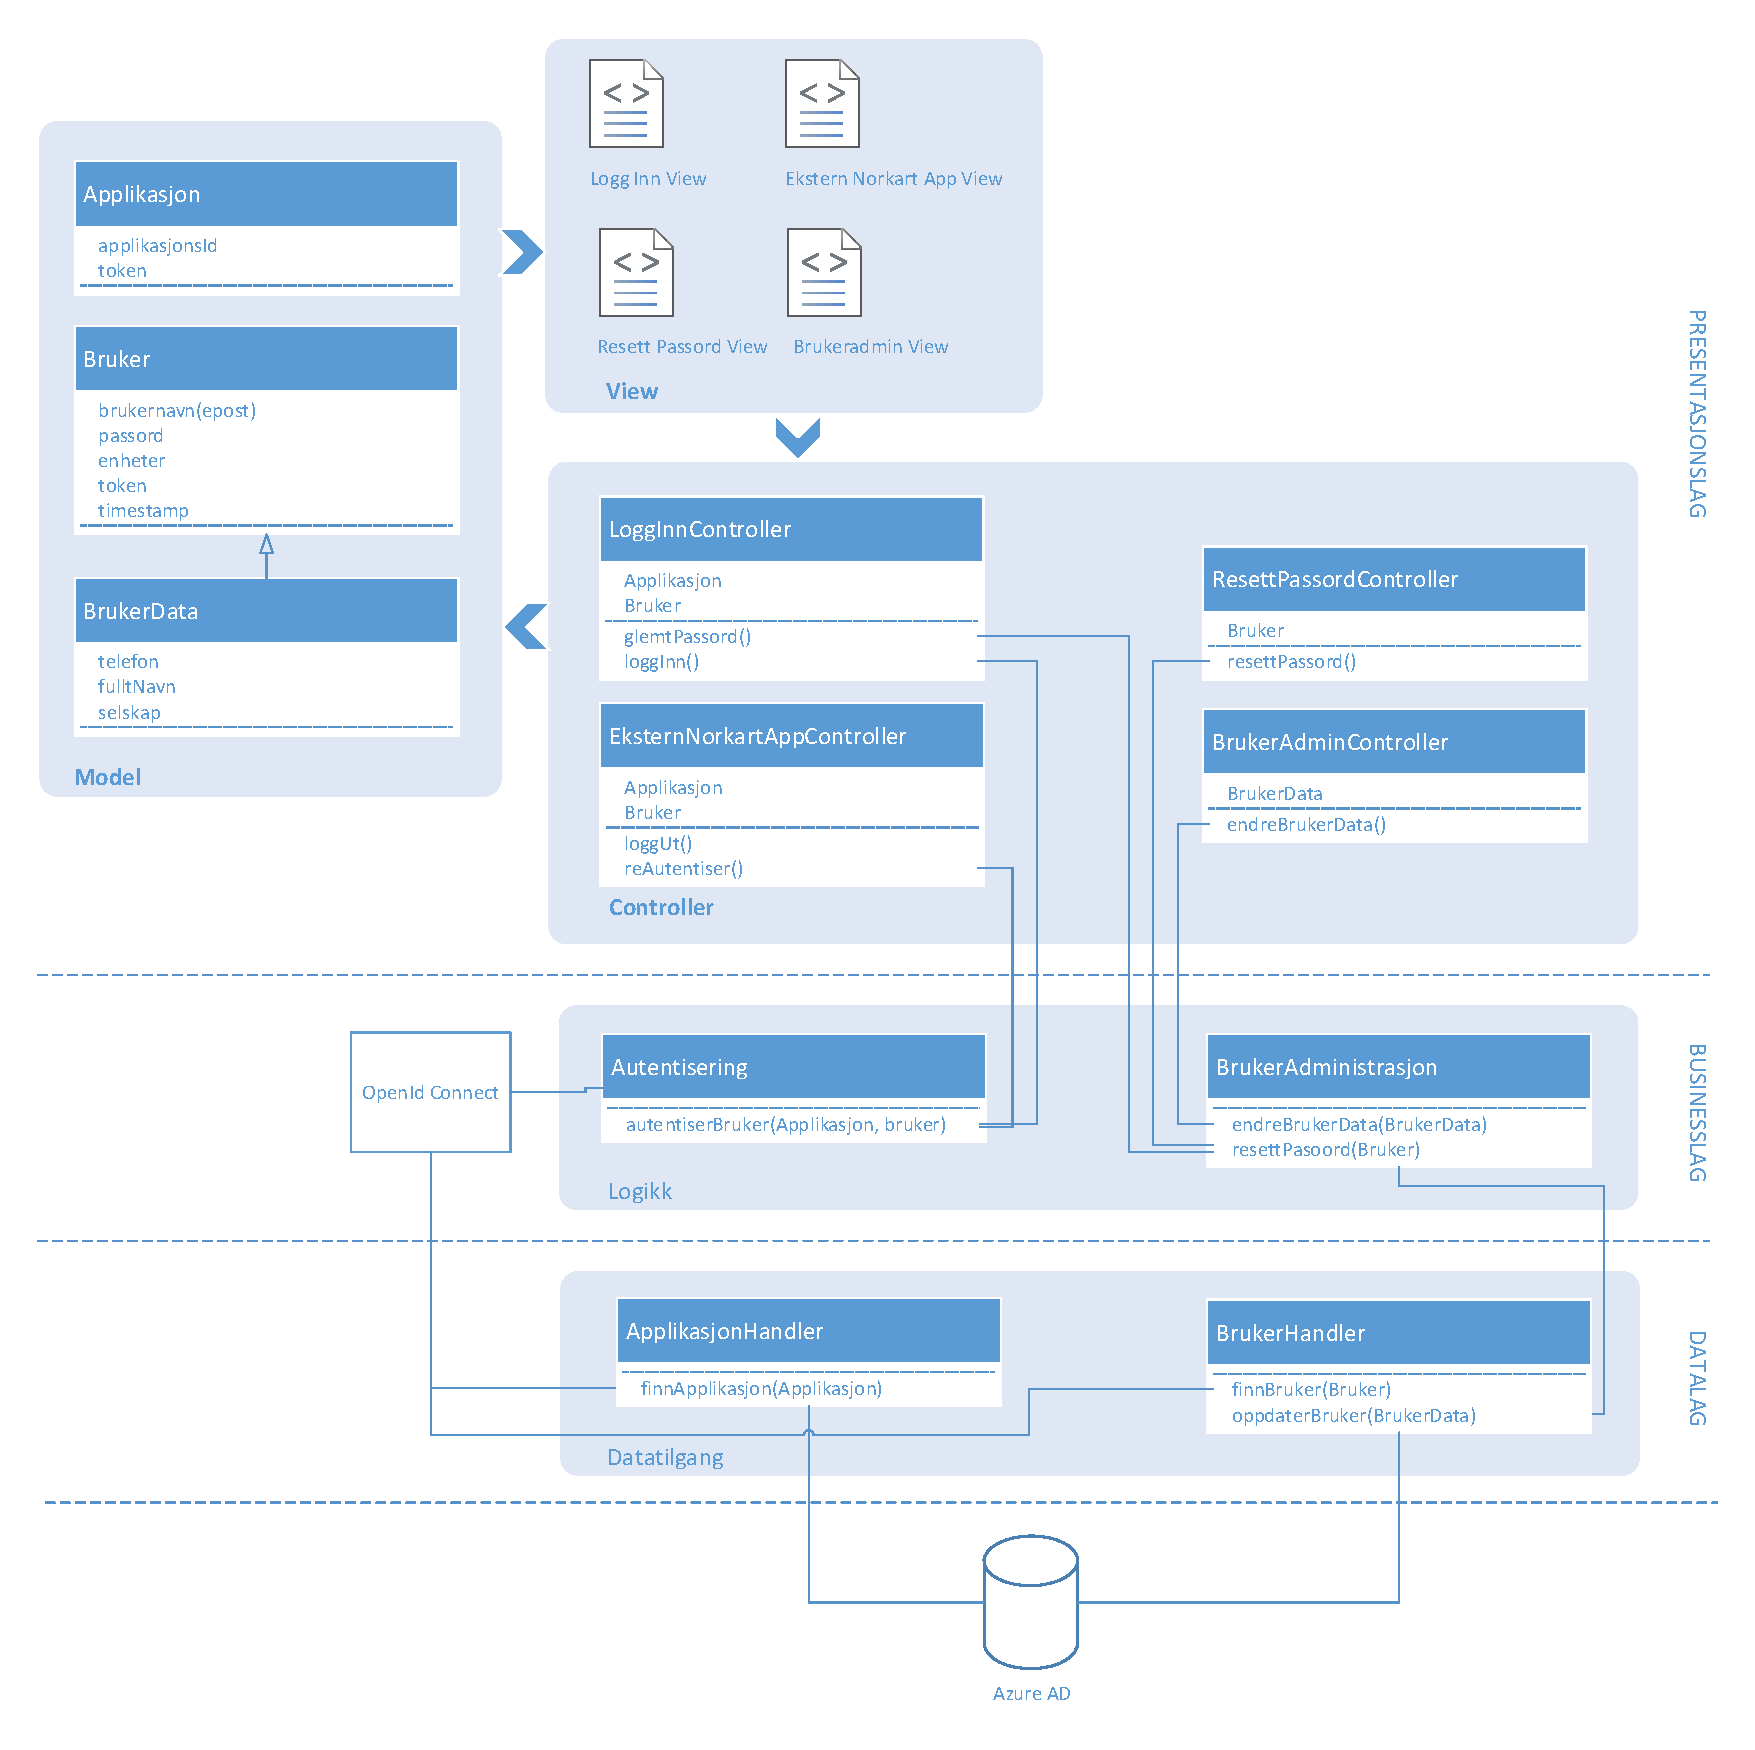
\includegraphics[scale=0.45]{graphics/04-arkitektur/LogiskViewKlassediagram}
    \caption{Klassediagram}
    \label{fig:LogiskViewKlassediagram}
\end{figure}

\subsection*{Trelagsarkitektur}
\label{subsec:logisk_view_trelagsarkitektur}
Klassediagrammet (se figur \ref{fig:LogiskViewKlassediagram}) viser at systemet er delt opp i et trelagssystem. Et trelagssystem muliggjør at hvert lag kan oppgraderes eller skiftes ut individuelt. Slik blir det billigere og enklere å endre systemet hvis det blir forandringer i kravene, eller det dukker opp ny teknologi som kan være mer hensiktsmessig å bruke. Lagene som er brukt er presentasjonslag, businesslag og datalag. Under står det beskrevet hva de tre lagene har ansvar for og hva de inneholder.
\newline
\subsection{Presentasjonslag}
\label{subsec:logisk_view_presentasjonslag}
Presentasjonslaget består av brukergrensesnittet og har som hovedmål å videreformidle input fra brukeren til resten av systemet og oppdatere brukergrensesnittet når input er behandlet. Det er bygd opp av et MVC pattern med fire views og fire tilhørende controllere. Systemet har i tillegg tre modell klasser.
\newline

\subsubsection{Views}
\label{subsec:logisk_view_views}
Viewene viser data til sluttbruker. Hvert view har sin controller som videreformidler input fra bruker nedover i arkitekturen.
\newline
\begin{itemize}
\item Logg Inn View
\newline Inneholder en glemt passord link og et logg inn skjema.
\item Ekstern Norkart App View
\newline En ekstern Norkart applikasjon brukere har logget seg inn på via Norkart ID. Her finnes en logg ut knapp.
Resett Passord View
\item Dette viewet inneholder muligheten til å resette passord. \newline Sluttbruker kan kun komme til dette viewet fra en link motatt i e-post under glemt passord funksjonalitet.
\item Egenadmin View
\newline Inneholder et skjema med brukerdata som brukeren kan endre på og oppdatere.
\end{itemize}

\bigskip
\subsubsection{Controllere}
\label{subsec:logisk_view_controllere}
Controllere informerer model og view om endrigner basert på input fra bruker. Klassediagrammet (se figur \ref{fig:LogiskViewKlassediagram}) viser hvilke klasser de forskjellige controllerne tilkaller på forskjellig input.
\newline
\begin{itemize}
\item Logg inn Controller 
\newline Starter glemt passord funskjonalitet og informerer businesslaget om at bruker vil logge seg inn.
\item Ekstern Norkart App Controller
\newline Setter i gang logg ut funskjonalitet. 
\item Resett Passord Controller
\newline Sier fra til businesslaget at bruker ønsker å resette sitt passord.
\item Egenadmin Controller 
\newline Sender ny brukerdata nedover i systemet for å oppdatere bruker.
\end{itemize}

\bigskip
\subsubsection{Modeller}
\label{subsec:logisk_view_modeller}
Systemet har tre modeller som brukes til å holde på data.
\newline
\begin{itemize}
\item Bruker
\newline Inneholder brukerens autentiserings data.
\item BrukerData
\newline Er et barn av bruker modellen og inneholder brukerens administrative data.
\item Applikasjon
\newline Inneholder applikasjonsdata til bruk i autentiseringsprosessen.
\end{itemize}

\subsection{Businesslag}
\label{subsec:logisk_view_buisnesslag}
Businesslaget har ansvar for logikken i systemet og mottar henvendelser fra presentasjonslaget. Det snakker også med klassene i datalaget for hendvendelser mot Azure AD. Systemet har to hovedklasser som styrer logikken i systemet.
\newline
\begin{itemize}
\item Autentisering
\newline Har ansvar for all logikken som må gjøres for at en bruker skal autentiseres mot sine applikasjoner.
\item EgenAdministrasjon
\newline Utøver all logikk som skal til for endring og oppdatering av bruker data.
\end{itemize}

\subsubsection{OpenID Connect}
\label{subsubsec:logsik_view_buisnesslag_openid_connect}
I tillegg til de to logikk klassene vil også OpenID Connect ligge i businesslaget. OpenID Connect brukes for å autentisere brukere.

\subsection{Datalag}
\label{subsec:logsik_view_datalag}
\labe{subsec:datalag}
Datalaget har ansvaret for alle henvendelser mot AzureAD og består av to hovedklasser.
\newline
\begin{itemize}
\item ApplikasjonHandler
\newline Sjekker om applikasjoner eksitsterer i Azure AD
\item BrukerHandler
\newline Sjekker om brukere eksisterer og oppdaterer brukerdata  i Azure AD
\end{itemize}

\section{Prosess View}
\label{sec:prosess_view}
\newline Som prosess view har vi valgt å lage activity diagram for de 4 overordnede use casene (se kapittel \ref{sec:use_case_view}). Activity diagram har til hensikt å illustrere arbeidsflyt, etter hendelser og valg når en oppgave skal gjennomføres. Vi har valgt å lage activity diagrammer for de fire kjerne funksjonene prosjektet initielt skal fokusere på.
\newline
\newline Begrepet applikasjonsserver1 brukes for å illustrere servere som kjører applikasjoner NorkartID autentiserer og autoriserer brukere for.
\newline

\subsection{Logge ut}
\label{subsec:prosess_view_logge_ut}
Activity diagram “Logge ut” (figur \ref{fig:ProsessViewLoggeUt}) begynner når en bruker sender en forespørsel til NorkartID serveren om å logge ut. For å kunne logge ut må brukeren bekrefte at det faktisk er brukeren som ønsker og logge ut. Dette gjøres for å beskytte mot at angripere kan kaste ut brukere fra  applikasjonene de er logget inn på. Avhengig av måten applikasjoner er koblet opp mot Norkart ID vil utgangsverdiene etter diagrammet ende opp i tre ulike tilstander. 

\begin{figure}[H]
\centering
    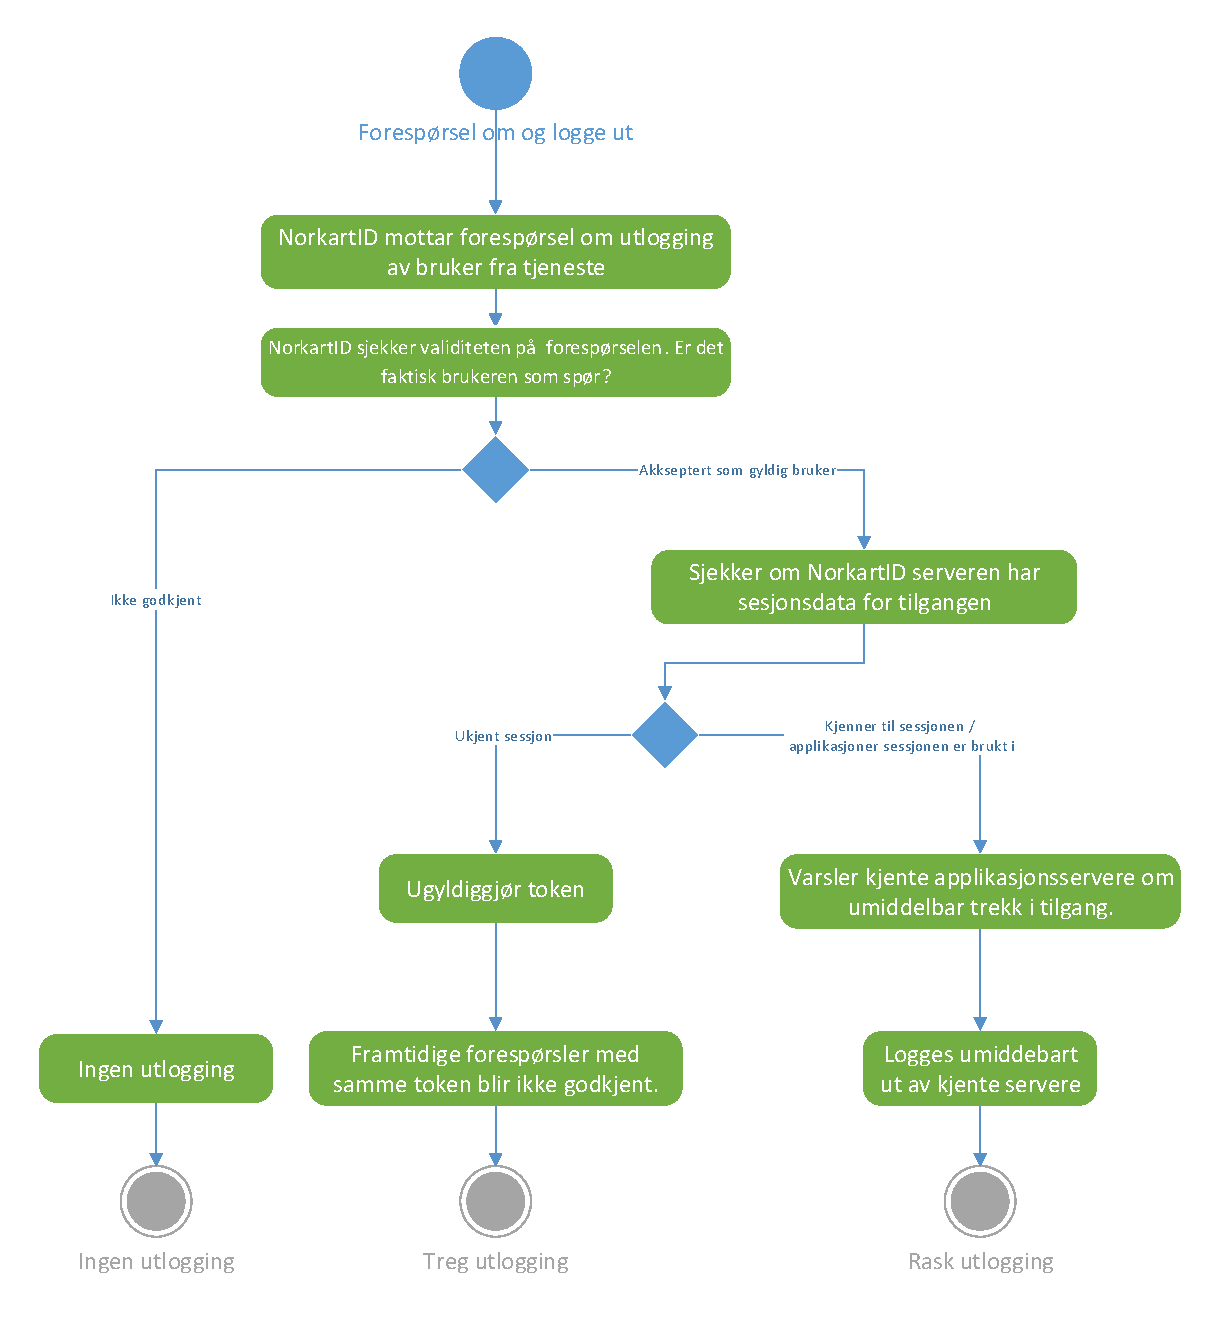
\includegraphics[scale=0.65]{graphics/04-arkitektur/ProsessViewLoggeUt}
    \caption{Activity diagram 'logge ut' }
    \label{fig:ProsessViewLoggeUt}
\end{figure}

\subsubsection*{Kommentar}
\label{subsubsec:prosess_view_logge_ut_kommentar}
Vi ser for oss at det kun er applikasjoner som støtter rask-utlogging fra applikasjon serveren som får lov til å dele access-token med andre prossesser. For de applikasjonene som kun støtter treg utlogging, anbefales bruk av egen access token, uten mulighet for å dele denne access token med andre applikasjoner. Dette vil føre til en egen pålogging før bruk, men vil øke sikkerheten bruker og Norkart. I oppgaven kommer vi ikke til å fokusere på denne problemstillingen innledende, men vil forsøke å dokumenter dette på best mulig måte for å gi Norkart grunnlag for en sikrest mulig bruk av tjenesten når på sikt tar systemet i bruk.
\newline

\subsection{Logge inn}
\label{subsec:prosess_view_logge_inn}
Activity diagramet påloggingsforespørselen (figur \ref{fig:ProsessViewLoggeInn}) begynner inngangsverdien etter at en bruker har sendt inn brukernavn og passord for å logge på en spesifikk tjeneste. Utgangsverdiene fra diagrammet er at brukeren blir logget inn eller avvist. Activity diagrammet tar ikke hensyn til eventuellt sikkerhets mekanismer som er lagt inn for å hindre brute-force pålogging på serveren. Dette vil vi likevel forsøke å implementere mekanismer mot, og vil trolig bygges inn som en del av de to første hendelsene etter inngangsverdien i diagrammet.
\newline

\subsection{Glemt passord}
\label{subsec:prosess_view_glemt_passord}
Activity diagrammet “glemt passord” (figur \ref{fig:ProsessViewGlemtPassord}) begynner etter at en bruker har skrevet inn en brukerid, muligens bekreftet at det faktisk er en bruker som forsøker å resette passordet, og ikke en datamaskin igjennom en captcha test. Prosessen innebærer at det sendes en mail til bruker som bruker må bekrefte innen 30 min for at resettingen av passordet skal være godkjent. Dersom samme bruker klikker på glemt passord flere ganger i løpet av en halvtime, uten og bekrefte på mail i mellomtiden, vil det kun være den siste mailen som ble sendt fra serveren som faktisk vil gi mulighet til å resette passordet. Eldre mail fra serveren vil da ugyldiggjøres. 
\newline

\subsection{Egenadministrasjon}
\label{subsec:prosess_view_egenadministrasjon}
Activity diagram “Egenadministrasjon (figur \ref{fig:ProsessViewEgenadministrasjon}) brukes for å illustrere når en bruker selv kan gjøre endringer av egne brukerprofildata. Inngangsverdien er at bruker skal logge inn på for å endre, første handling er at bruker logger på id.norkart.no. Vi forutsetter at dette fører til en vellykket innlogging. Utgangsverdien er at brukeren, enten bruker har endret brukerprofildata eller ikke, logger ut, eller forlater id.norkart.no.
\newline

\begin{figure}[H]
\centering
    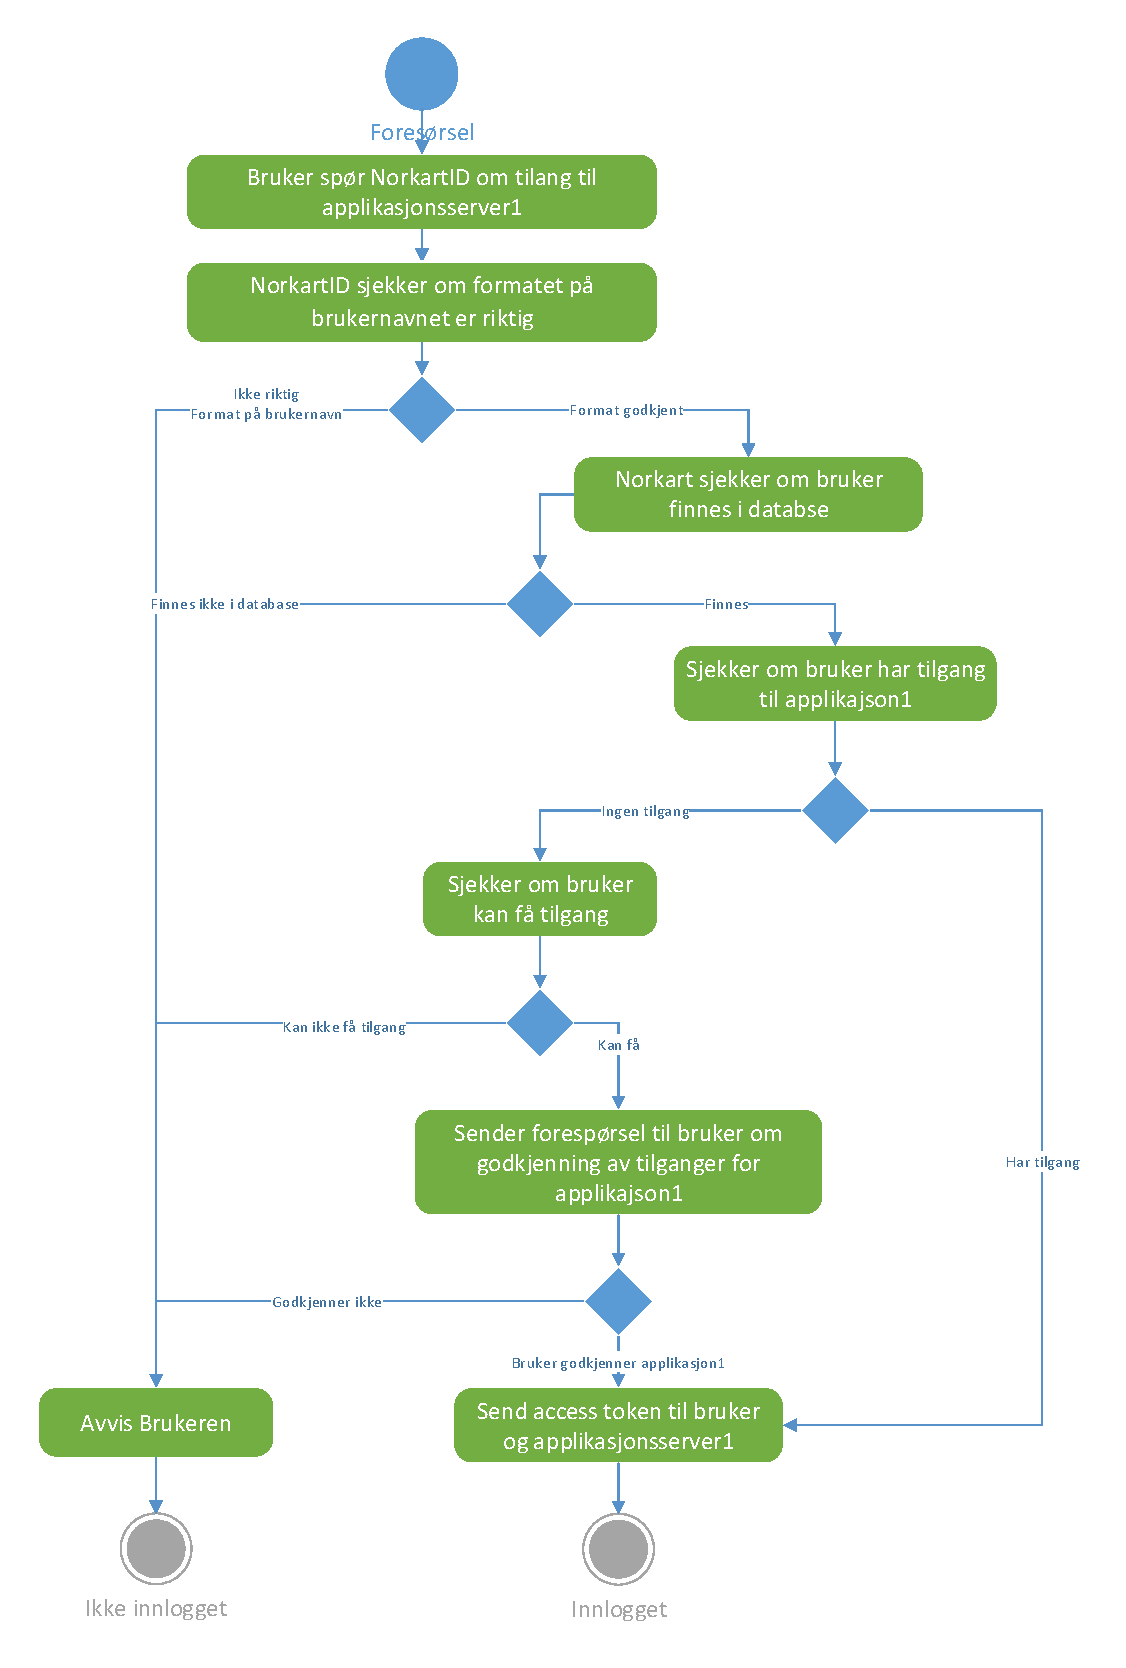
\includegraphics[scale=0.65]{graphics/04-arkitektur/ProsessViewLoggeInn}
    \caption{Activity diagram 'logge inn' }
    \label{fig:ProsessViewLoggeInn}
\end{figure}

\begin{figure}[H]
\centering
    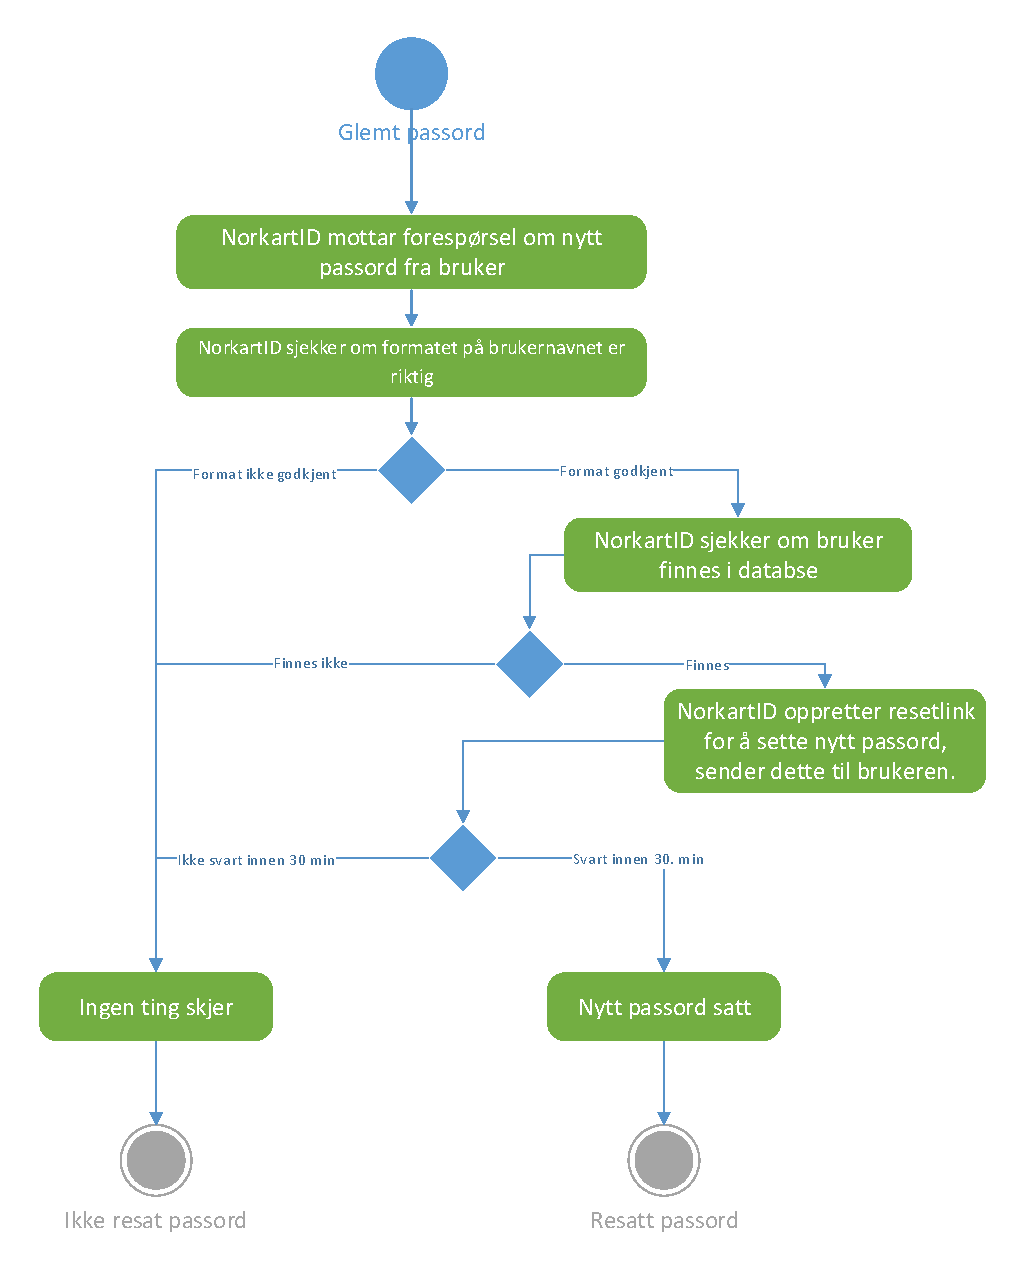
\includegraphics[scale=0.65]{graphics/04-arkitektur/ProsessViewGlemtPassord}
    \caption{Activity diagram 'glemt passord' }
    \label{fig:ProsessViewGlemtPassord}
\end{figure}

\begin{figure}[H]
\centering
    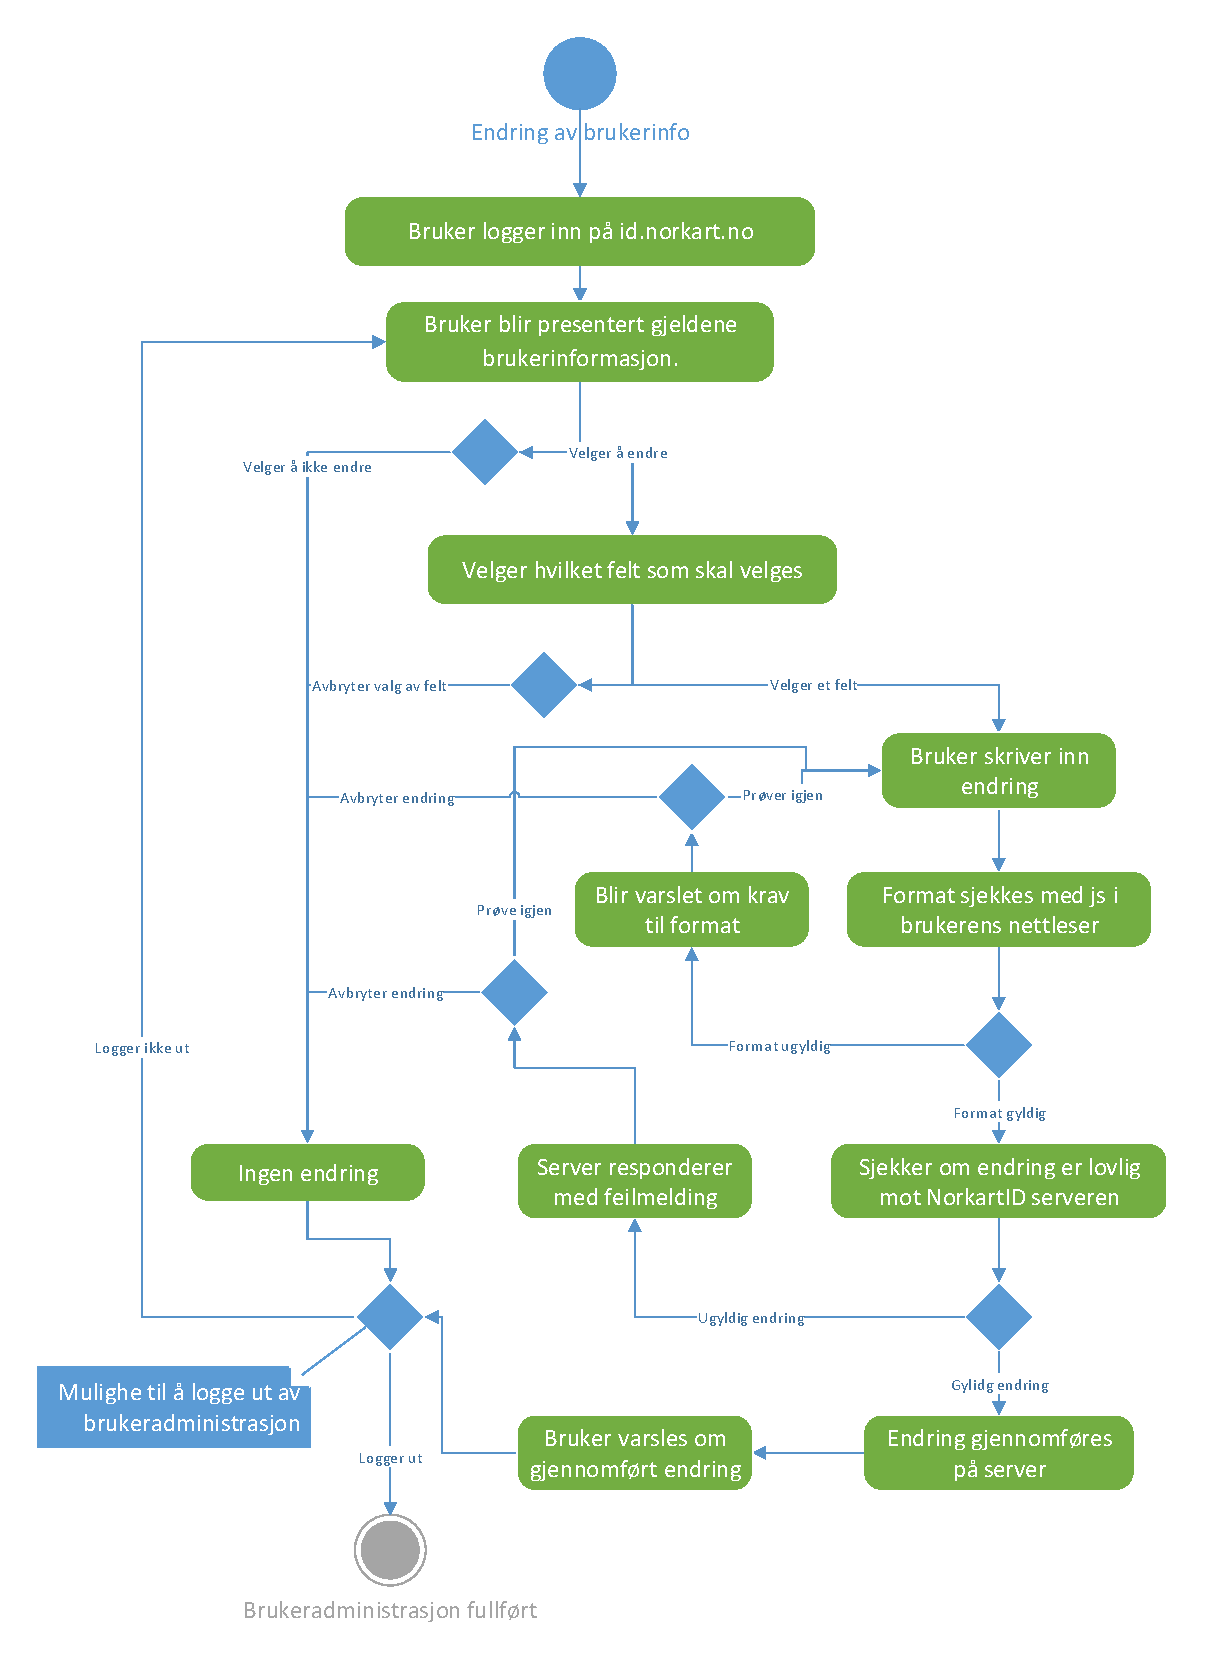
\includegraphics[scale=0.65]{graphics/04-arkitektur/ProsessViewEgenadministrasjon}
    \caption{Activity diagram 'egenadministrasjon' }
    \label{fig:ProsessViewEgenadministrasjon}
\end{figure}

\section{Utviklings View}
\label{sec:utviklings_view}
Dette viewet har til hensikt å illustrere systemet fra en programmerers perspektiv. Dette er gjort ved å lage et komponent diagram, se figur \ref{fig:UtviklingsViewDevelopmentView}. Systemet består av flere komponenter som er avhengig av hverandre for å fungere. For å kunne bruke systemet er webserveren avhengig av Norkart ID. Norkart ID vil fungere som hovedkomponent. For å kunne logge inn og autentisere brukere er Norkart ID avhengig av OpenID Connect for autentisering og en Azure AD for å finne brukere og hvilke applikasjoner disse har tilgang til. Norkart ID er i tillegg avhenig av en Azure AD for å administrere brukere. Hvis en bruker har glemt sitt passord må Norkart ID kontakte en epost server.  Norkart ID inneholder i tillegg to komponenter, nemlig Bruker Administrasjon og Autentisering. Bruker Administrasjon er avhengig av at brukeren er autentisert for å kunne utføre sine oppgaver.

\begin{figure}[H]
    \centering
    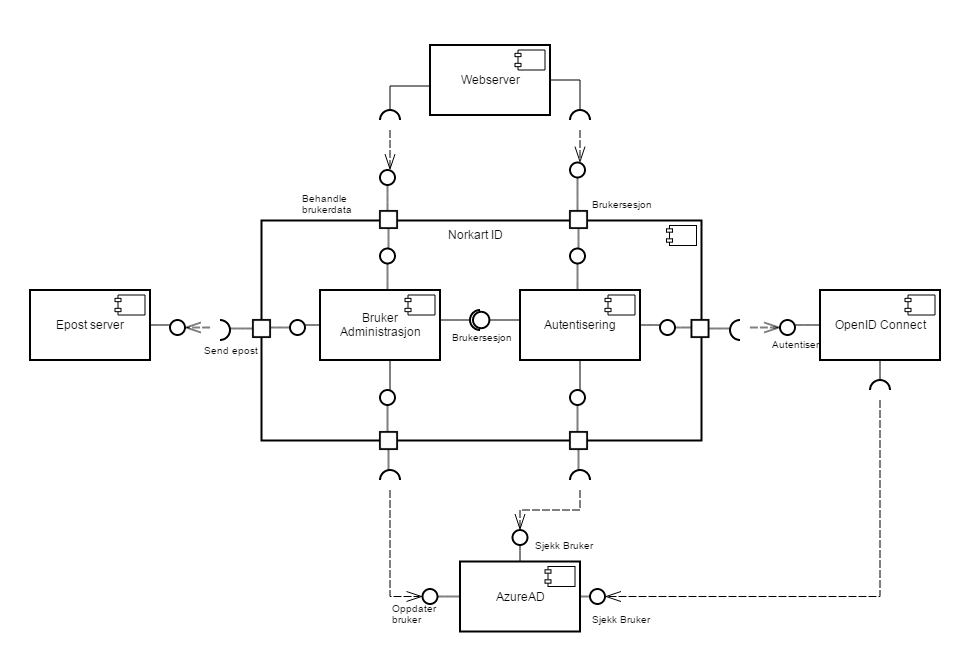
\includegraphics[scale=0.40]{graphics/04-arkitektur/UtviklingsViewKomponentDiagram.png}
    \caption{Komponent diagram over Norkart ID }
    \label{fig:UtviklingsViewKomponentDiagram}
\end{figure}

\section{Distribusjons View}
\label{sec:distribusjons_view}
AHensikten med distribusjons view er å illustrere hvordan systemet skal settes opp i forhold til hardware implementasjon. Ettersom hele Norkart ID er planlagt å kjøre på virituelle maskiner i Norkart sin nettsky, illustrerer vi bare distribusjons view med tre elementer i distribusjons diagrammet (se figur \ref{fig:UtviklingsViewDistribusjonsDiagram}). Vi regner Bruker som en betegnelse på brukere av systemet.  Applikasjoner i diagrammet er de applikasjonene Norkart ID skal gi brukeren tilgang til, altså de Norkart ID skal autentisere og autorisere tilganger for. Den markerte rammen rundt "Azure AD" og "Norkart ID med OpenID Connect" skal illustrere at systemet ligger virituelt på en sky. Når applikasjoner ligger utenfor skyen betyr dette bare at det stilles ingen krav til at applikasjonene må være en del av den samme skyen, eller kjøre på de samme serverene. 

\begin{figure}[H]
    \centering
    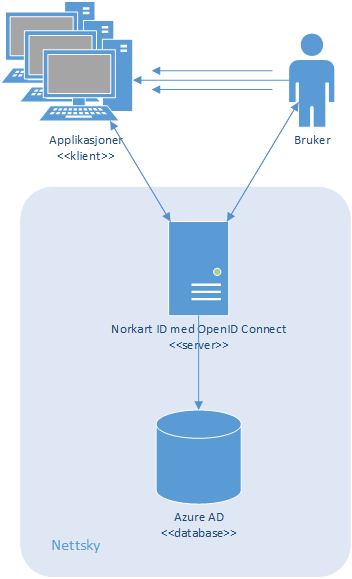
\includegraphics[scale=0.55]{graphics/04-arkitektur/UtviklingsViewDistribusjonsDiagram.png}
    \caption{Distribusjons diagram for Norkart ID }
    \label{fig:UtviklingsViewDistribusjonsDiagram}
\end{figure}
\chapter{Konklusjon}
\label{chap:konklusjon}
{\color{red}TODO}
Intro til kapitlet. 

\section{Sammenfatning av løsning}
\label{sec:konklusjon_sammefatningAvLosning}
{\color{red}TODO}
Trekk slutninger relater med hva vi anbefaler Norkart å gjøre.
Do's and dont's
Hent ut hva vi anbefaler Norkart å gjøre ut ifra det som står nevnt i kap. 5, 6 og 7. Snakk også om kap 8 sine tutorials.

\section{Sammenfatning av testresultater}
\label{sec:konklusjon_sammenfatningAvTestresultater}
{\color{red}TODO}
Trekk slutninger fra hva testresultatene betyr.
Trekk fram brukeranalysen.
Oppsette av Azure fra Microsoft

\section{Prosjektoppgaven}
\label{sec:konklusjon_prosjektoppgaven}
{\color{red}TODO}
Læringsutbytte
Prosessen
Gruppesamarbeidet?
Hvordan det var, hvordan det føltes, hva vi kunne gjort annerledes, problemer underveis
Begrunne hvorfor vi har den strukturen vi har på rapporten?
Fordeling av arbeidet
Arbeidsform
Kanskje vurdere å legge inn veien videre

\section{Avvik, endringer og justeringer av oppgaven}
\label{sec:konklusjon_avvikEndringOgJusteringer}
{\color{red}TODO}
Tanker og slutninger relatert med endringer i oppgaven. 
Hva vi fikk til
Hva vi ikke fikk til.
Hvilke justeringer vi måtte gjøre og hvorfor. Trekk slutninger om dette hadde store betydninger for oppgava, for oss og for Norkart.

\section{Oppdragsgivers syn på leveransen}
\label{sec:konklusjon_oppdragsgiversSynPåLeveransen}
{\color{red}TODO}
Her klarer vi kun å gjengi det som Norkart har sagt om oppgaven så dette blir litt spekulasjonsrelatert.
Innspill fra Einar, Håkon, Grete og Yngve?
Inntrykk av utbytte til Norkart fra rapporten?



\input{101-underskrifter}

\bibliographystyle{gucthesis}
\bibliography{references}

\appendix
\chapter{Termonologi}
\label{app:termonologi}


\sec{SingleSignOn} 
\label{app:termonologi_singleSignOn}
Et brukernavn og passord for flere løsninger. Kan også bety at når du har logget inn et sted, så vil du automatisk logges inn andre steder levert av samme tjenestetilbyder, uten å trenge å skrive brukernavn og passord på nytt.


\chapter{Arbeidsmetode}
\label{app:arbeidsmetode}
I dette vedlegget beskrives det hvordan prosjektgruppen planla og satt sammen en utviklingsmetode inspirert av MVP og Scrum. Denne plannen ble satt opp helt i begynnelsen av prosjektperioden. 

\subsection{Arbeidsmetodikk}
\label{app:arbeidsmetode_arbeidsmetodikk}
Ettersom oppdraget skal ferdiggjøres på kun noen måneder er det valgt å bruke en smidig utviklingsmodell. Dette passer også godt overens med at prosjektgruppen er på kun tre personer. Produktet skal utvikles med teknologier som er ukjente både for oppdragsgiver og prosjektgruppen, derfor kan endringshyppigheten være stor under utvikling. Med en smidig utviklingsmodell kan det brukes iterasjoner for å hele tiden kunne endre på prototypen uten at det får for store konsekvenser. Fordi utviklingstiden for oppdraget er relativt kort ble det anbefalt av oppdragsgiver å bruke elementer fra Lean Startup. Derfor kommer gruppen til å bruke  Minimum Viable Product (MVP)\footnote{En versjon av produktet som dekker kundens behov og går gjennom en Lean Startup iterasjon med minst mulig bruk av ressurser og tid} og varierende iterasjoner fra Lean Startup. Varierende iterasjoner muliggjør tidlig og ofte levering av en fungerende prototype til oppdragsgiver. I tillegg vil det brukes elementer fra Scrum siden alle i gruppen er godt kjent med Scrum og oppdragsgiver bruker modellen mye i deres utviklingsprosjekter. I hovedsak kommer vi til å bruke rollene, møter og "product backlog" fra Scrum.
\\
\\
Kort oppsummert, Scrum vil bli brukt til alt rundt iterasjonene, mens selve iterasjonene vil være bygd opp av elementer fra Lean Startup.
\\
\\
Selv om utviklingen skal skje med varierende iterasjoner er det satt noen beslutningspunkter underveis i utviklingen, dette for å skape en visshet om at utviklingen går fremover. Under disse beslutningspunktene vil det holdes demomøter for oppdragsgiver. I tillegg vil det gjøres en release av prototypen til oppdragsgiver. Fordi gruppen skal utvikle en prototype og ikke et ferdig produkt vil det ikke bli gjort releaser til sluttbruker underveis.
\\
\\
Ettersom prosjektet er en del av bacheloroppgaven til gruppen kreves dokumentasjon på arbeidet som gjøres underveis. Som nevnt vil Scrum sin "product backlog" benyttes. Denne vil bestå av PBIer knyttet til user stories i kravspesifikasjonen og elementer knyttet til rapporten. For å dokumentere design og arkitekturfasen vil Rational Unified Process(RUP) sitt Software Architecture Document(SAD) bli benyttet. For å dokumentere utviklingsprosessen vil det bli skrevet møtereferater fra planleggingsmøter, vurderingsmøter, retrospektive møter og demomøter.

\pagebreak
\begin{figure}[!htbp]
    \begin{center}
        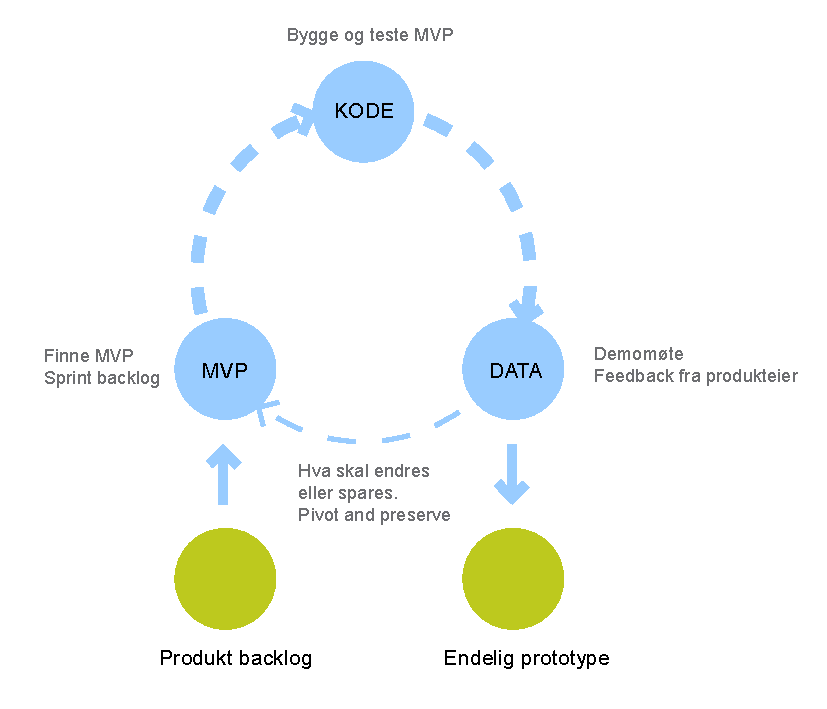
\includegraphics[scale=0.80]{graphics/UtviklingsModell}
        \caption{Utviklingsmodell for Norkart ID}
        \label{fig:utviklingsmodell}
    \end{center}
\end{figure}

\subsection{Iterasjonssirkel}
\label{app:arbeidsmetode_arbeidsmetodikk_iterasjonssirkerl}
Hver iterasjon vil bestå av sirkelen vist i figur \ref{fig:utviklingsmodell}. En iterasjon er ferdig når MVP har gått gjennom denne sirkelen. Sirklen er definert av prosjektgruppen med inspirert av "lean startup" og "Scrum".

\subsection*{MVP}
Den første fasen i iterasjonen er MVP. I denne fasen vil det holdes et planleggingsmøte hvor målet er å definere en MVP for oppkommende sprint.

\subsubsection*{KODE}
I kodefasen skal MVP utvikles og testes.

\subsubsection*{DATA}
Data er den siste fasen i en iterasjon. Her skal det holdes et gjennomgangsmøte hvor resultatet av iterasjonen presenteres for oppdragsgiver og oppdragsgiver gir så tilbakemelding. I tillegg vil det holdes et retrospektivt møte her. 
\\
\\
Etter datafasen i iterasjonen er gjort vil det holdes et endringsmøte hvor gruppen må bestemme om utviklingen kan gå videre i neste iterasjon eller om MVP må endres eller gjøres på nytt.

\subsection{Roller}
\label{app:arbeidsmetode_arbeidsmetodikk_roller}
Gruppen kommer til å bruke roller fra Scrum. Oppdragsgiver stiller med produkteier og Scrum master (omtalt som veileder), mens medlemmene i gruppa er team medlemmer.


\subsection{Møter}
\label{app:arbeidsmetode_arbeidsmetodikk_møter}
Under utvikling av Norkart ID vil det holdes en del møter. Dette blir gjort for å skape oversikt og opprettholde et godt samarbeid. I tillegg vil disse møtene brukes som dokumentering av utviklingsprosessen.

\subsection*{Planleggingsmøte}
\bigskip{}
\begin{tabular}{l p{11cm}}
    Når: & I MVP fasen \\
    Deltagere: & Gruppen \\
    Hensikt: & Fastsette en MVP og hvilke tasker som trengs for å utvikle denne i kommende sprint
\end{tabular}

\subsection*{Gjennomgangsmøte}
\bigskip{}
\begin{tabular}{l p{11cm}}
    Når: & I datafasen \\
    Deltagere: & Gruppen og oppdragsgiver \\
    Hensikt: & Presentere utviklet MVP for oppdragsgiver. Oppdragsgiver gir tilbakemelding på MVP.
\end{tabular}

\subsection*{Retrospektivtmøte}
\bigskip{}
\begin{tabular}{l p{11cm}}
    Når: & I datafasen \\
    Deltagere: & Gruppen \\
    Hensikt: & Gjennomgang av utviklingsperioden som har vært og finne eventuelle endringer som bør gjøres før neste iterasjon. Dette har til hensikt å skape overblikk over fremdrift
\end{tabular}

\subsection*{Endringsmøte}
\bigskip{}
\begin{tabular}{l p{11cm}}
    Når: & Mellom to sprinter \\
    Deltagere: & Gruppen \\
    Hensikt: & Bestemmer om utviklingen kan gå videre eller om MVP må endres eller gjøres på nytt.
\end{tabular}

\subsection*{Demomøte}
\bigskip{}
\begin{tabular}{l p{11cm}}
    Når: & Under hvert beslutningspunkt \\
    Deltagere: & Gruppen og oppdragsgiver \\
    Hensikt: & Demomøte av prototype holdes for oppdragsgiver. Oppdragsgiver får i tilleg en release av prototypen.
\end{tabular}
\bigskip{}
I tillegg til møtene nevnt ovenfor kommer gruppen til å ha møte med veiledere en gang i uken, så fremt det er nødvendig. Gruppen kommer også til benytte seg av Scrums daglige møter og det vil holdes statusmøter hver mandag.


\chapter{Møtereferater sprint 1}

\section{Planleggingsmøte}
\label{app:MotereferaterSprint1_planleggingsmote}
24 /2 - 25/2 
 
\subsection{Saksliste}

\textbf{Del 1:}
\begin{itemize}
\item Velge PBI for oppkommende sprint 
\item Opprette tasker til PBI  
\item Hva skal leveres, ikke hvordan vi skal gjøre det 
\item Estimer taskene i timer 
\item Ingen tasks over 8 timer 
\item Finne "the definition of done" for tasker 
\end{itemize}
\\ 
\textbf{Del 2:}
\begin{itemize}
\item Prioritere tasks
\item Finne MVP basert på tasker 
\item Fastsette hvor lenge sprinten skal vare 
\end{itemize}

\subsection{Referat}
\textbf{Del 1: 24/2-2015}
\\Oppmøte: Ida, Alf, PC
\\Lengde: 5 timer 
\\
\begin{itemize}
\item Valgt PBI for sprint 1: Logg Inn 
\item Lagd tasks til PBIen
\item Definert hva "done" er for hver task 
\item Estimert tasks 
\end{itemize}
\bigskip
\textbf{Del 2: 25/2-2015 }
\\Oppmøte: Ida, Alf, PC
\\Lengde: 2 timer 
\\
\begin{itemize}
\item Prioritert tasks 
\item Finne MVP 
\item - MVP skal inneholde et proof of concept på å logge inn med OpenID Connect ved bruk av Thinctecture
\item - IdentityServer 3 og skal bruke Azure AD som AD 
\item Sprint 1 varer i 2 uker 24/2 - 9/3 
\\MVP Fasen: 24/2 og 25/2 
\\Kode Fasen: 26/2 til 8/3 
\\Data Fasen: 9/3 
\end{itemize}


\section{Gjennomgangsmøte }
\label{app:MotereferaterSprint1_gjennomgangsmote}
5/3-2015 
\\Oppmøte: Ida, PC, Alf, Einar og Håkon 
\\Lengde: 1 time 
 
\subsection{Saksliste}
\begin{itemize}
\item Presentere  MVP (demo av Azure AD i bruk med OpenID Connect)
\item Diskutere funn fra sprint 
\item Få tilbakemelding fra oppdragsgiver 
\end{itemize}

\subsection{Referat}
\begin{itemize}
\item Gruppen har funnet ut at Azure AD inneholder mye av funksjonaliteten Norkart ønsker. Det vil derfor ikke bli nødvendig å programmere en middelvare 
\item Norkart ønsker derfor at vi skal konsentrere oppgaven rundt anvendelse av Azure AD for Norkart
\item Norkart bekreftet for oss at punktet om lokal hosting bortfaller fra oppgaven 
\end{itemize}


\section{Endringsmøte }
\label{app:MotereferaterSprint1_endringsmote}
9/3-2015 
\\Oppmøte: Ida, Alf, PC
\\Lengde: 1 time 
 
\subsection{Saksliste}
\begin{itemize}
\item Bestemme om MVP kan fortsettes på, må endres eller om den skal forkastes basert på gjennomgangsmøte med Norkart 5/3 og gruppens funn under sprint 1.
\end{itemize}

 
\subsection{Referat}
\begin{itemize}
\item MVP ble utviklet som planlagt, uten bruk av Thinctecture IdentityServer 3 
\item MVP kan fortsettes på slik den er i dag, men kommer til å spille en mye mindre rolle i endelig løsning enn planlagt. 
\item MVP skal bygges videre på ved å teste om all funksjonalitet fungerer som den skal. 
\end{itemize}


\section{Retrospektivt møte}
\label{app:MotereferaterSprint1_retrospektivmote}
9/3-2015 
\\Oppmøte: Ida, Alf, PC
\\Lengde: 1 time 
 
\subsection{Saksliste}
\begin{itemize}
\item Gå gjennom hvordan gruppen har jobbet sammen i forhold til utviklingsmetode og roller. 
\item Bestemme om noe skal endres, legges til eller fjernes til neste sprint 
\end{itemize}


\subsection{Referat}
\begin{itemize}
\item Gruppen er usikre på om det er hensiktsmessig å bruke MVP nå som det ikke skal programmeres et produkt.
\item Det ble bestemt og holde på variende iterasjoner og bruken av MVP i neste sprint. 
\item Rollene til alle i gruppen fungerer og skal fortsatt holdes.  
\item Det er for mange møter i hver sprint, derfor ble det bestemt at endringsmøte og retrospektivt møte slåes sammen til et møte. 
\item Istedet for å opprette tasker for en hel PBI på planleggingsmøte skal det kun opprettes tasker på planlagte MVP.
\end{itemize}


\chapter{Møtereferater sprint 2}

\section{Planleggingsmøte}
\label{app:MotereferaterSprint2_planleggingsmote}
9/3-2015 
\\Oppmøte: Ida, Alf, PC
\\Lengde: 2 timer 
 
\subsection{Saksliste}
\begin{itemize}
\item Velge PBI for oppkommende sprint 
\item Finne MVP 
\item Opprette tasker til MVP  
\item Hva skal leveres, ikke hvordan vi skal gjøre det 
\item Estimer taskene i timer 
\item Ingen tasks over 8 timer 
\item Finne "the definition of done" for tasker 
\item Fastsette hvor lang sprinten skal 
\end{itemize}

\subsection{Referat}
\begin{itemize}
\item Valgt PBI for MVP: Proof of concept og dokumentasjon 
\\ Proof of concept skal inneholde: 
    \begin{itemize}
    \item Logg inn  
    \item Logg ut 
    \item Resette passord  
    \item Brukeradm 
    \item Registrering 
    \end{itemize}
\item Opprettet tasker for MVP, se TFS 
\item Sprint 2 skal vare i 6 dager 
\end{itemize}


\section{Endrings og retrospektivt møte}
\label{app:MotereferaterSprint2_endringsOgRetrospektivMote}
17/3-2015 
\\Oppmøte: Alf, Ida, PC
\\Lengde: 1 timer 
 
\subsection{Saksliste}
\begin{itemize}
\item Bestemme om MVP kan fortsettes på, må endres eller om den skal forkastes basert på demomøte med Norkart 16/3. 
\item Gå gjennom hvordan gruppen har jobbet sammen i forhold til utviklingsmetode og roller.
\item Bestemme om noe skal endres, legges til eller fjernes til neste sprint.
\end{itemize}

\subsection{Referat }
\begin{itemize}
\item MVP ble ikke helt ferdig, men den kan fortsettes på i neste sprint 
\item Neste sprint må være lenger
\item Vi går brort fra MVP ettersom utviklingen har tatt en annen vending, vi bruker nå heller sprint mål. 
\item Tasks skal ikke tildeles til personer på planleggingsmøte, men heller taes når folk skal jobbe med dette. 
\item Vi skal prøve å legge til så mange estimerte tasks som trengs for å kommendesprint, men det er også lov til å legge til tasks mitt i sprinten. 
\end{itemize} 



\end{document}